\documentclass[letterpaper,10pt,titlepage]{custbook}
%
\pagestyle{headings}
%
\usepackage{amsmath}
\usepackage{amsfonts}
\usepackage{amssymb}
\usepackage[ansinew]{inputenc}
\usepackage[OT1]{fontenc}
\usepackage{graphicx}
\usepackage{longtable}
\usepackage{makeidx}
%
%Packages that must go in the document preamble.
\makeindex
%
%Define certain conspicuous global constants.
\newcommand{\productbasenamelong}{Embedded Tool Set}
\newcommand{\productbasenameshort}{EMTS}
\newcommand{\productversion}{0.1.0}
\newcommand{\productname}{\productbasenameshort{}-\productversion}
%
%Shared mathematical definitions
% $Header: /home/dashley/cvsrep/uculib01/uculib01/doc/manual/comps/workmdef.tex,v 1.2 2007/08/30 14:25:20 dtashley Exp $
%
%%Sets of real numbers.
\newcommand{\vworkrealset}{{\mathbb{R}}}
\newcommand{\vworkrealsetnonneg}{{\mathbb{R}^+}}
%
%%Sets of integers.
\newcommand{\vworkintset}{{\mathbb{Z}}}
\newcommand{\vworkintsetnonneg}{{\mathbb{Z}^+}}
\newcommand{\vworkintsetpos}{{\mathbb{N}}}
%
%%Sets of rational numbers.
\newcommand{\vworkratset}{{\mathbb{Q}}}
\newcommand{\vworkratsetnonneg}{{\mathbb{Q}^+}}
%
%%Sets of irrational numbers.
\newcommand{\vworkirratset}{{\mathbb{error}}}
\newcommand{\vworkirratsetnonneg}{{\mathbb{error}^+}}
%
%%"Divides" and "Not Divides".  Am not able to find quite
%%the right symbol for "Not Divides" at this time.
\newcommand{\vworkdivides}{\mid}
\newcommand{\vworknotdivides}{\hspace{-0.125em}\not\hspace{0.245em}\mid\hspace{0.135em}}
%%
%%The implication operator, which may change throughout the work.  Both a horizontal
%%and vertical form are defined.
\newcommand{\vworkhimp}{\to}
\newcommand{\vworkvimp}{\downarrow}
%%
%%The symbol for logical equivalence.  There are three forms defined, the standard,
%%the long, and the short, which may be identical.
\newcommand{\vworkequiv}{\leftrightarrow}
\newcommand{\vworkshortequiv}{\leftrightarrow}
\newcommand{\vworklongequiv}{\longleftrightarrow}
\newcommand{\vworkvertequiv}{\updownarrow}

%$Log: workmdef.tex,v $
%Revision 1.2  2007/08/30 14:25:20  dtashley
%Edits.
%
%Revision 1.1  2007/08/30 14:24:32  dtashley
%Initial checkin.
%
%End of $RCSfile: workmdef.tex,v $.
%
%Hyphenation exceptions
%$Header: svn://localhost/dtapublic/pubs/books/ucbka/trunk/volshare/workhxcp.tex 274 2019-08-11 21:43:05Z dashley $
%
%This file contains hyphenation exceptions for work.
\hyphenation{EEPROM}
\hyphenation{MATLAB}
\hyphenation{SIMULINK}
\hyphenation{UPPAAL}
%
%End of file WORKHXCP.TEX

%
%New environments, etc.
%$Header: /home/dashley/cvsrep/uculib01/uculib01/doc/manual/comps/worknenv.tex,v 1.5 2010/01/27 16:08:53 dashley Exp $
%
%%%%%%%%%%%%%%%%%%%%%%%%%%%%%%%%%%%%%%%%%%%%%%%%%%%%%%%%%%%%%%%%%%%%%%%%%%%%%
%% SEPARATORS
%%%%%%%%%%%%%%%%%%%%%%%%%%%%%%%%%%%%%%%%%%%%%%%%%%%%%%%%%%%%%%%%%%%%%%%%%%%%%
%%
%Digit separation distance for denoting thousands, etc.  Choosing space rather than comma.
\newcommand{\vworkthousandsdigsepinmathmode}{\;}
%%
%%%%%%%%%%%%%%%%%%%%%%%%%%%%%%%%%%%%%%%%%%%%%%%%%%%%%%%%%%%%%%%%%%%%%%%%%%%%%
%% CHAPTER QUOTES
%%%%%%%%%%%%%%%%%%%%%%%%%%%%%%%%%%%%%%%%%%%%%%%%%%%%%%%%%%%%%%%%%%%%%%%%%%%%%
%%
%Quote which begins each chapter.
\newcommand{\beginchapterquote}[2]{\textbf{#1}\begin{flushright}\emph{---#2}\end{flushright}}

%Source when included with quote which begins each chapter.
\newcommand{\chapquoteshortsrc}[1]{\begin{flushright}\emph{---#1}\end{flushright}}
%%
%%%%%%%%%%%%%%%%%%%%%%%%%%%%%%%%%%%%%%%%%%%%%%%%%%%%%%%%%%%%%%%%%%%%%%%%%%%%%
%% EXAMPLES
%%%%%%%%%%%%%%%%%%%%%%%%%%%%%%%%%%%%%%%%%%%%%%%%%%%%%%%%%%%%%%%%%%%%%%%%%%%%%
%%
%General-purpose example start.  Used to generate the beginning of the example
%only, should enclose only an optional label.
\newtheorem{vworkgenexample}{Example}

%General-purpose example solution start.
\newcommand{\vworkgenexamplesolutionhead}{\noindent\textbf{Solution: }}

%General-purpose example solution body.  This is the environment in which
%the example's solution is stated.  For the present time, there are no
%changes to the text.
\newenvironment{vworkgenexamplesolutionbody}{\noindent\textbf{Solution: }}{}

%Define a new counter used to hold the example number within a chapter.
%\newcounter{vworkexamplecounter}[chapter]

%Alternate numbering for examples.
%\renewcommand{\thevworkexamplecounter}{\thechapter.\arabic{vworkexamplecounter}}

%Define the marking which delimits the start of an example.  For now, this
%is a little bit of space and a horizontal bar.
\newcommand{\vworkexampleheader}{\par\nopagebreak\vspace{0.01in}%
                                 \noindent\rule{\textwidth}{1pt}%
                                 \par\nopagebreak}

%Define the marking which delimits the end of an example.  For now, this is
%a horizontal line.  An example must be "footed" manually because there are
%so many variations on what can be in an example.
\newcommand{\vworkexamplefooter}{\par\nopagebreak%
                                 \vspace{0.01in}\noindent\rule{\textwidth}{1pt}%
                                 \par\nopagebreak}

%Define a new environment to hold the body of an example, and the numbering of an
%example.
\newenvironment{vworkexamplestatement}%
               {\vworkexampleheader\noindent%
               \setlength{\parindent}{0em}%
               \setlength{\parskip}{1ex}%
               \refstepcounter{vworktheoremcounter}%
               \textbf{Example \nopagebreak[2]\thevworktheoremcounter{}: }}{\par}

%Define a new environment to hold a "solution" or "remarks" block within an example.
%The presence or absence of a colon is something that may change, so better to code
%that in here.
\newenvironment{vworkexampleparsection}[1]{\par\noindent%
               \setlength{\parindent}{0em}%
               \setlength{\parskip}{1ex}%
               \textbf{#1:\nopagebreak[2] }}{\par}
%%
%%%%%%%%%%%%%%%%%%%%%%%%%%%%%%%%%%%%%%%%%%%%%%%%%%%%%%%%%%%%%%%%%%%%%%%%%%%%%
%% DEFINITIONS
%%%%%%%%%%%%%%%%%%%%%%%%%%%%%%%%%%%%%%%%%%%%%%%%%%%%%%%%%%%%%%%%%%%%%%%%%%%%%
%%
%Counter for "artifical" theorems.  In this context, "artificial" means that the
%built-in theorem environment is not used.
%\newcounter{vworkdefinitioncounter}[chapter]

%Alternate numbering for definitions.
%\renewcommand{\thevworkdefinitioncounter}{\thechapter.\arabic{vworkdefinitioncounter}}

%Define the markings which delimit the start and ends of a definition.  For now, these
%are NULL.  Later, I may define something else--a little extra space or a line.
\newcommand{\vworkdefinitionheader}{\par\nopagebreak%
                                    \vspace{0.01in}\noindent\rule{\textwidth}{1pt}%
                                    \par\nopagebreak}
\newcommand{\vworkdefinitionfooter}{\par\nopagebreak%
                                    \vspace{0.01in}\noindent\rule{\textwidth}{1pt}%
                                    \par\nopagebreak}

%Environment to hold definitions.  This was defined (rather than using the built-in
%environment) because I cannot stand having a number without a colon.
\newenvironment{vworkdefinitionstatement}%
               {\vworkdefinitionheader\noindent%
               \setlength{\parindent}{0em}%
               \setlength{\parskip}{1ex}%
               \refstepcounter{vworktheoremcounter}%
               \textbf{Definition \nopagebreak[2]\thevworktheoremcounter{}: }}{\par}

%Environment to begin a definition that also has descriptive text.
\newenvironment{vworkdefinitionstatementpar}[1]%
               {\vworkdefinitionheader\noindent%
               \setlength{\parindent}{0em}%
               \setlength{\parskip}{1ex}%
               \refstepcounter{vworktheoremcounter}%
               \textbf{Definition \nopagebreak[2]\thevworktheoremcounter{} (#1): }}{\par}

%Define a new environment to hold a "solution" or "remarks" block within a definition.
%The presence or absence of a colon is something that may change, so better to code
%that in here.
\newenvironment{vworkdefinitionparsection}[1]{\par\noindent%
               \setlength{\parindent}{0em}%
               \setlength{\parskip}{1ex}%
               \textbf{#1:\nopagebreak[2] }}{\par}
%%
%%%%%%%%%%%%%%%%%%%%%%%%%%%%%%%%%%%%%%%%%%%%%%%%%%%%%%%%%%%%%%%%%%%%%%%%%%%%%
%% LEMMAS
%%%%%%%%%%%%%%%%%%%%%%%%%%%%%%%%%%%%%%%%%%%%%%%%%%%%%%%%%%%%%%%%%%%%%%%%%%%%%
%%
%% Because lemmas and theorems are so similar, decided that they should
%% use the same counters.  I think this makes it easier for readers, so they
%% don't have to separate the two out when searching.
%%
%\newcounter{vworktheoremcounter}[chapter]

%Alternate numbering for lemmas.
%\renewcommand{\thevworktheoremcounter}{\thechapter.\arabic{vworktheoremcounter}}

%Define the markings which delimit the start and ends of a lemma.  For now, these
%are NULL.  Later, I may define something else--a little extra space or a line.
\newcommand{\vworklemmaheader}{\par\nopagebreak%
                               \vspace{0.01in}\noindent\rule{\textwidth}{1pt}%
                               \par\nopagebreak}
\newcommand{\vworklemmafooter}{\par\nopagebreak%
                               \vspace{0.01in}\noindent\rule{\textwidth}{1pt}%
                               \par\nopagebreak}

%Environment to hold lemmas.  This was defined (rather than using the built-in
%environment) because I cannot stand having a number without a colon.
\newenvironment{vworklemmastatement}%
               {\vworklemmaheader\noindent%
               \setlength{\parindent}{0em}%
               \setlength{\parskip}{1ex}%
               \refstepcounter{vworktheoremcounter}%
               \textbf{Lemma \nopagebreak[2]\thevworktheoremcounter{}: }}{\par}

%Environment to begin a lemma that also has descriptive text.
\newenvironment{vworklemmastatementpar}[1]%
               {\vworklemmaheader\noindent%
               \setlength{\parindent}{0em}%
               \setlength{\parskip}{1ex}%
               \refstepcounter{vworktheoremcounter}%
               \textbf{Lemma \nopagebreak[2]\thevworktheoremcounter{} (#1): }}{\par}

%Define a new environment to hold the proof of a lemma.
\newenvironment{vworklemmaproof}%
               {\par\noindent%
               \setlength{\parindent}{0em}%
               \setlength{\parskip}{1ex}%
               \textbf{Proof:\nopagebreak[2] }}{\hfill\rule{1.5ex}{1.5ex}\par}

%Define a new environment to hold a "solution" or "remarks" block within a lemma.
%The presence or absence of a colon is something that may change, so better to code
%that in here.
\newenvironment{vworklemmaparsection}[1]{\par\noindent%
               \setlength{\parindent}{0em}%
               \setlength{\parskip}{1ex}%
               \textbf{#1:\nopagebreak[2] }}{\par}
%%
%%%%%%%%%%%%%%%%%%%%%%%%%%%%%%%%%%%%%%%%%%%%%%%%%%%%%%%%%%%%%%%%%%%%%%%%%%%%%
%% THEOREMS
%%%%%%%%%%%%%%%%%%%%%%%%%%%%%%%%%%%%%%%%%%%%%%%%%%%%%%%%%%%%%%%%%%%%%%%%%%%%%
%%
%Counter for "artifical" theorems.  In this context, "artificial" means that the
%built-in theorem environment is not used.
\newcounter{vworktheoremcounter}[chapter]

%Alternate numbering for theorems.
\renewcommand{\thevworktheoremcounter}{\thechapter.\arabic{vworktheoremcounter}}

%Define the markings which delimit the start and ends of a theorem.  For now, these
%are NULL.  Later, I may define something else--a little extra space or a line.
\newcommand{\vworktheoremheader}{\par\nopagebreak%
                                 \vspace{0.01in}\noindent\rule{\textwidth}{1pt}%
                                 \par\nopagebreak}
\newcommand{\vworktheoremfooter}{\par\nopagebreak%
                                 \vspace{0.01in}\noindent\rule{\textwidth}{1pt}%
                                 \par\nopagebreak}

%Environment to hold theorems.  This was defined (rather than using the built-in
%environment) because I cannot stand having a number without a colon.
\newenvironment{vworktheoremstatement}%
               {\vworktheoremheader\noindent%
               \setlength{\parindent}{0em}%
               \setlength{\parskip}{1ex}%
               \refstepcounter{vworktheoremcounter}%
               \textbf{Theorem \nopagebreak[2]\thevworktheoremcounter{}: }}{\par}

%Environment to begin a theorem that also has descriptive text.
\newenvironment{vworktheoremstatementpar}[1]%
               {\vworktheoremheader\noindent%
               \setlength{\parindent}{0em}%
               \setlength{\parskip}{1ex}%
               \refstepcounter{vworktheoremcounter}%
               \textbf{Theorem \nopagebreak[2]\thevworktheoremcounter{} (#1): }}{\par}

%Define a new environment to hold the proof of a theorem.
\newenvironment{vworktheoremproof}%
               {\par\noindent%
               \setlength{\parindent}{0em}%
               \setlength{\parskip}{1ex}%
               \textbf{Proof:\nopagebreak[2] }}{\hfill\rule{1.5ex}{1.5ex}\par}

%Define a new environment to hold a "solution" or "remarks" block within a theorem.
%The presence or absence of a colon is something that may change, so better to code
%that in here.
\newenvironment{vworktheoremparsection}[1]{\par\noindent%
               \setlength{\parindent}{0em}%
               \setlength{\parskip}{1ex}%
               \textbf{#1:\nopagebreak[2] }}{\par}
%%
%%%%%%%%%%%%%%%%%%%%%%%%%%%%%%%%%%%%%%%%%%%%%%%%%%%%%%%%%%%%%%%%%%%%%%%%%%%%%
%% ALGORITHMS
%%%%%%%%%%%%%%%%%%%%%%%%%%%%%%%%%%%%%%%%%%%%%%%%%%%%%%%%%%%%%%%%%%%%%%%%%%%%%
%%
%Counter for "artifical" theorems.  In this context, "artificial" means that the
%built-in theorem environment is not used.
%\newcounter{vworktheoremcounter}[chapter]

%Alternate numbering for theorems.
%\renewcommand{\thevworktheoremcounter}{\thechapter.\arabic{vworktheoremcounter}}

%Define the markings which delimit the start and ends of an algorithm.  For now, these
%are NULL.  Later, I may define something else--a little extra space or a line.
\newcommand{\vworkalgorithmheader}{\par\nopagebreak%
                                 \vspace{0.01in}\noindent\rule{\textwidth}{1pt}%
                                 \par\nopagebreak}
\newcommand{\vworkalgorithmfooter}{\par\nopagebreak%
                                 \vspace{0.01in}\noindent\rule{\textwidth}{1pt}%
                                 \par\nopagebreak}

%Environment to hold algorithms.  This was defined (rather than using the built-in
%environment) because I cannot stand having a number without a colon.
\newenvironment{vworkalgorithmstatement}%
               {\vworkalgorithmheader\noindent%
               \setlength{\parindent}{0em}%
               \setlength{\parskip}{1ex}%
               \refstepcounter{vworktheoremcounter}%
               \textbf{Algorithm \nopagebreak[2]\thevworktheoremcounter{}: }}{\par}

%Environment to begin an algorithm that also has descriptive text.
\newenvironment{vworkalgorithmstatementpar}[1]%
               {\vworkalgorithmheader\noindent%
               \setlength{\parindent}{0em}%
               \setlength{\parskip}{1ex}%
               \refstepcounter{vworktheoremcounter}%
               \textbf{Algorithm \nopagebreak[2]\thevworktheoremcounter{} (#1): }}{\par}

%Define a new environment to hold the proof of an algorithm.
\newenvironment{vworkalgorithmproof}%
               {\par\noindent%
               \setlength{\parindent}{0em}%
               \setlength{\parskip}{1ex}%
               \textbf{Proof:\nopagebreak[2] }}{\hfill\rule{1.5ex}{1.5ex}\par}

%Define a new environment to hold a "solution" or "remarks" block within an algorithm.
%The presence or absence of a colon is something that may change, so better to code
%that in here.
\newenvironment{vworkalgorithmparsection}[1]{\par\noindent%
               \setlength{\parindent}{0em}%
               \setlength{\parskip}{1ex}%
               \textbf{#1:\nopagebreak[2] }}{\par}
%The "itemize" environment defined by the book style files didn't seem to have
%quite the right appearance for presenting our algorithms.  For this reason, the
%following environments were defined.  Level 0 is flush left with bullets, Level 1
%is slightly more indented, etc.
\newenvironment{alglvl0}{\begin{list}
               {$\bullet$}{\setlength{\labelwidth}{3mm}\setlength{\leftmargin}{6mm}}}
               {\end{list}}
\newenvironment{alglvl1}{\begin{list}
               {$\bullet$}{\setlength{\labelwidth}{3mm}\setlength{\leftmargin}{6mm}}}
               {\end{list}}
\newenvironment{alglvl2}{\begin{list}
               {$\bullet$}{\setlength{\labelwidth}{3mm}\setlength{\leftmargin}{6mm}}}
               {\end{list}}
%The environments above have been obsoleted.
\newcounter{alglvl0ctr}
\newenvironment{algblvl0}{\begin{list}
               {\textbf{[\arabic{alglvl0ctr}]}}{\usecounter{alglvl0ctr}%
               \setlength{\labelwidth}{6mm}\setlength{\leftmargin}{9mm}}}
               {\end{list}}
%%
%%%%%%%%%%%%%%%%%%%%%%%%%%%%%%%%%%%%%%%%%%%%%%%%%%%%%%%%%%%%%%%%%%%%%%%%%%%%%
%% EXERCISES
%%%%%%%%%%%%%%%%%%%%%%%%%%%%%%%%%%%%%%%%%%%%%%%%%%%%%%%%%%%%%%%%%%%%%%%%%%%%%
%%
%Counter for exercises at the end of each chapter.
\newcounter{vworkexercisecounter}[chapter]

%We'd like to number an exercise slightly differently, using the chapter number
%followed by "." followed by the equation number.
\renewcommand{\thevworkexercisecounter}{\thechapter.\arabic{vworkexercisecounter}}

%Define the markings which delimit the start and ends of an exercise.  For now, these
%are NULL.  Later, I may define something else--a little extra space or a line.
\newcommand{\vworkexerciseheader}{\par\vspace{0.01in}\par}
\newcommand{\vworkexercisefooter}{\par\vspace{0.01in}\par}

%Environment to hold exercises.
\newenvironment{vworkexercisestatement}%
               {\vworkexerciseheader\noindent%
               \setlength{\parindent}{0em}%
               \setlength{\parskip}{1ex}%
               \refstepcounter{vworkexercisecounter}%
               \textbf{[\thevworkexercisecounter{}]}\nopagebreak[2] }{\par}

%Define a new environment to hold a "remarks" block within an exercise.
%The presence or absence of a colon is something that may change, so better to code
%that in here.
\newenvironment{vworkexerciseparsection}[1]{\par\noindent%
               \setlength{\parindent}{0em}%
               \setlength{\parskip}{1ex}%
               \textbf{#1: }}{\par}
%%
%%%%%%%%%%%%%%%%%%%%%%%%%%%%%%%%%%%%%%%%%%%%%%%%%%%%%%%%%%%%%%%%%%%%%%%%%%%%%
%% LESSONS LEARNED
%%%%%%%%%%%%%%%%%%%%%%%%%%%%%%%%%%%%%%%%%%%%%%%%%%%%%%%%%%%%%%%%%%%%%%%%%%%%%
%%
%Counter for lessons learned.
\newcounter{vworklessonslearnedcounter}[chapter]

%Alternate numbering for lessons learned.
\renewcommand{\thevworklessonslearnedcounter}{\thechapter.\arabic{vworklessonslearnedcounter}}

%Define the markings which delimit the start and ends of a lesson learned.
\newcommand{\vworklessonslearnedheader}{\par\nopagebreak%
                                 \vspace{0.01in}\noindent\rule{\textwidth}{1pt}%
                                 \par\nopagebreak}
\newcommand{\vworklessonslearnedfooter}{\par\nopagebreak%
                                 \vspace{0.01in}\noindent\rule{\textwidth}{1pt}%
                                 \par\nopagebreak}

%Environment to hold lessons learned.
\newenvironment{vworklessonslearnedstatement}%
               {\vworklessonslearnedheader\noindent%
               \setlength{\parindent}{0em}%
               \setlength{\parskip}{1ex}%
               \refstepcounter{vworklessonslearnedcounter}%
               \textbf{Lesson Learned \nopagebreak[2]\thevworklessonslearnedcounter{}: }}{\par}
%%
%%%%%%%%%%%%%%%%%%%%%%%%%%%%%%%%%%%%%%%%%%%%%%%%%%%%%%%%%%%%%%%%%%%%%%%%%%%%%
%% QUOTES
%%%%%%%%%%%%%%%%%%%%%%%%%%%%%%%%%%%%%%%%%%%%%%%%%%%%%%%%%%%%%%%%%%%%%%%%%%%%%
%%
%Environment to hold quotes.
\newenvironment{indentedquote}{\begin{quote}}{\end{quote}}
%%
%%%%%%%%%%%%%%%%%%%%%%%%%%%%%%%%%%%%%%%%%%%%%%%%%%%%%%%%%%%%%%%%%%%%%%%%%%%%%
%% EXERCISE SOLUTIONS
%%%%%%%%%%%%%%%%%%%%%%%%%%%%%%%%%%%%%%%%%%%%%%%%%%%%%%%%%%%%%%%%%%%%%%%%%%%%%
%%
%Environment To Hold A Solution To An Exercise
\newenvironment{vworkexercisesolution}[1]{\par\noindent%
               \setlength{\parindent}{0em}%
               \setlength{\parskip}{1ex}%
               \textbf{Solution To Exercise #1}\par}{\par}

%Command which begins section of solutions for each chapter, command which
%separates solutions, and command which ends solutions in each chapter.
\newcommand{\vworkexercisechapterheader}{\par\nopagebreak\vspace{0.01in}%
                                 \noindent\rule{\textwidth}{1pt}%
                                 \par\nopagebreak}
\newcommand{\vworkexerciseseparator}{\par\nopagebreak\vspace{0.01in}%
                                 \noindent\rule{\textwidth}{1pt}%
                                 \par\nopagebreak}
\newcommand{\vworkexercisechapterfooter}{\par\nopagebreak%
                                 \vspace{0.01in}\noindent\rule{\textwidth}{1pt}%
                                 \par\nopagebreak}
%%
%%%%%%%%%%%%%%%%%%%%%%%%%%%%%%%%%%%%%%%%%%%%%%%%%%%%%%%%%%%%%%%%%%%%%%%%%%%%%
%% GLOSSARY OF TERMS
%%%%%%%%%%%%%%%%%%%%%%%%%%%%%%%%%%%%%%%%%%%%%%%%%%%%%%%%%%%%%%%%%%%%%%%%%%%%%
%5
%The following environment is for the glossary of terms at the end.
\newenvironment{vworktermglossaryenum}{\begin{list}
               {}{\setlength{\labelwidth}{0mm}
                  \setlength{\leftmargin}{4mm}
                  \setlength{\itemindent}{-4mm}
                  \setlength{\parsep}{0.85mm}}}
               {\end{list}}
%%
%%%%%%%%%%%%%%%%%%%%%%%%%%%%%%%%%%%%%%%%%%%%%%%%%%%%%%%%%%%%%%%%%%%%%%%%%%%%%
%% GLOSSARY OF MATHEMATICAL TERMS
%%%%%%%%%%%%%%%%%%%%%%%%%%%%%%%%%%%%%%%%%%%%%%%%%%%%%%%%%%%%%%%%%%%%%%%%%%%%%
%%
%The following environment is for the glossary of mathematical terms at the end.
\newenvironment{vworkmathtermglossaryenum}{\begin{list}
               {}{\setlength{\labelwidth}{0mm}
                  \setlength{\leftmargin}{4mm}
                  \setlength{\itemindent}{-4mm}
                  \setlength{\parsep}{0.85mm}}}
               {\end{list}}

%%%%%%%%%%%%%%%%%%%%%%%%%%%%%%%%%%%%%%%%%%%%%%%%%%%%%%%%%%%%%%%%%%%%%%%%%%%%%%%%%%%%%%%%%%
%%%%%%%%%%%%%%%%%%%%%%%%%%%%%%%%%%%%%%%%%%%%%%%%%%%%%%%%%%%%%%%%%%%%%%%%%%%%%%%%%%%%%%%%%%
% TCL COMMAND DOCUMENTATION
%
%Environment to hold the "NAME" portion of a Tcl command description.
\newenvironment{tclcommandname}[1]{\noindent\textbf{NAME}\vspace{-1.0ex}\begin{list}%
               {}{\setlength{\leftmargin}{0.25in}}\item\textbf{#1}---}{\end{list}}

%Command to display a synopsis line inside the synopsis environment.
\newcommand{\tclcommandsynopsisline}[2]{\par\textbf{#1} \textit{#2}\par}

%Environment to hold the "SYNOPSIS" portion of a Tcl command description.
\newenvironment{tclcommandsynopsis}{\noindent\textbf{SYNOPSIS}\vspace{-1.0ex}\begin{list}%
               {}{\setlength{\leftmargin}{0.25in}}\item{}}{\end{list}}

%Environment to hold the "DESCRIPTION" portion of a Tcl command description.
\newenvironment{tclcommanddescription}{\noindent\textbf{DESCRIPTION}\vspace{-1.0ex}\begin{list}%
               {}{\setlength{\leftmargin}{0.25in}}\item{}}{\end{list}}

%Environment to hold the "ACKNOWLEDGEMENTS" portion of a Tcl command description.
\newenvironment{tclcommandacknowledgements}{\noindent\textbf{ACKNOWLEDGEMENTS}\vspace{-1.0ex}\begin{list}%
               {}{\setlength{\leftmargin}{0.25in}}\item{}}{\end{list}}

%Environment to hold a specific subdescription within the DESCRIPTION--useful for enumerating
%possible legal commands and command forms.
\newenvironment{tclcommandinternaldescription}{\noindent{}\vspace{-5.0ex}\begin{list}%
               {}{\setlength{\leftmargin}{0.25in}}\item{}}{\end{list}}

%Command to use to format a command prototype preceding the environment above (i.e. a synopsis).
\newcommand{\tclcommanddescsynopsisline}[2]{\par\textbf{#1} \textit{#2}\par}

%Environment to hold the "USAGE NOTES" portion of a Tcl command description.
\newenvironment{tclcommandusagenotes}{\noindent\textbf{USAGE NOTES}\vspace{-1.0ex}\begin{list}%
               {}{\setlength{\leftmargin}{0.25in}}\item{}}{\end{list}}

%Environment to hold the "SAMPLE INVOCATIONS" portion of a TCL command or extension description.
\newenvironment{tclcommandsampleinvocations}{\noindent\textbf{SAMPLE INVOCATIONS}\vspace{-1.0ex}\begin{list}%
               {}{\setlength{\leftmargin}{0.25in}}\item{}}{\end{list}}

%Environment to hold the "SEE ALSO" portion of a TCL command or extension utility description.
\newenvironment{tclcommandseealso}{\noindent\textbf{SEE ALSO}\vspace{-1.0ex}\begin{list}%
               {}{\setlength{\leftmargin}{0.25in}}\item{}}{\end{list}}

%%%%%%%%%%%%%%%%%%%%%%%%%%%%%%%%%%%%%%%%%%%%%%%%%%%%%%%%%%%%%%%%%%%%%%%%%%%%%%%%%%%%%%%%%%
%%%%%%%%%%%%%%%%%%%%%%%%%%%%%%%%%%%%%%%%%%%%%%%%%%%%%%%%%%%%%%%%%%%%%%%%%%%%%%%%%%%%%%%%%%
% DOS COMMAND-LINE UTILITY DOCUMENTATION
%
%Environment to hold the "NAME" portion of a DOS command-line utility.
\newenvironment{dosutilcommandname}[1]{\noindent\textbf{NAME}\vspace{-1.0ex}\begin{list}%
               {}{\setlength{\leftmargin}{0.25in}}\item\textbf{#1}---}{\end{list}}

%Command to display a synopsis line inside the synopsis environment.
\newcommand{\dosutilcommandsynopsisline}[2]{\par\textbf{#1} \textit{#2}\par}

%Environment to hold the "SYNOPSIS" portion of a DOS command-line utility description.
\newenvironment{dosutilcommandsynopsis}{\noindent\textbf{SYNOPSIS}\vspace{-1.0ex}\begin{list}%
               {}{\setlength{\leftmargin}{0.25in}}\item{}}{\end{list}}

%Environment to hold the "DESCRIPTION" portion of a DOS command-line utility description.
\newenvironment{dosutilcommanddescription}{\noindent\textbf{DESCRIPTION}\vspace{-1.0ex}\begin{list}%
               {}{\setlength{\leftmargin}{0.25in}}\item{}}{\end{list}}

%Environment to hold the "ACKNOWLEDGEMENTS" portion of a DOS command-line utility description.
\newenvironment{dosutilcommandacknowledgements}{\noindent\textbf{ACKNOWLEDGEMENTS}\vspace{-1.0ex}\begin{list}%
               {}{\setlength{\leftmargin}{0.25in}}\item{}}{\end{list}}

%Environment to hold a specific subdescription within the DESCRIPTION--useful for enumerating
%possible legal commands and command forms.
\newenvironment{dosutilcommandinternaldescription}{\noindent{}\vspace{-5.0ex}\begin{list}%
               {}{\setlength{\leftmargin}{0.25in}}\item{}}{\end{list}}

%Command to use to format a command prototype preceding the environment above (i.e. a synopsis).
\newcommand{\dosutilcommanddescsynopsisline}[2]{\par\textbf{#1} \textit{#2}\par}

%Environment to hold the "USAGE NOTES" portion of a DOS command-line utility description.
\newenvironment{dosutilcommandusagenotes}{\noindent\textbf{USAGE NOTES}\vspace{-1.0ex}\begin{list}%
               {}{\setlength{\leftmargin}{0.25in}}\item{}}{\end{list}}

%Environment to hold the "REMARKS" portion of a DOS command-line utility description.
\newenvironment{dosutilcommandremarks}{\noindent\textbf{REMARKS}\vspace{-1.0ex}\begin{list}%
               {}{\setlength{\leftmargin}{0.25in}}\item{}}{\end{list}}

%Environment to hold the "COMMAND-LINE OPTIONS" portion of a DOS command-line utility description.
\newenvironment{dosutilcommandcommandlineoptions}{\noindent\textbf{COMMAND-LINE OPTIONS}\vspace{-1.0ex}\begin{list}%
               {}{\setlength{\leftmargin}{0.25in}}\item{}}{\end{list}}

%Environment to hold the "SAMPLE INVOCATION" portion of a DOS command-line utility description.
\newenvironment{dosutilcommandsampleinvocations}{\noindent\textbf{SAMPLE INVOCATIONS}\vspace{-1.0ex}\begin{list}%
               {}{\setlength{\leftmargin}{0.25in}}\item{}}{\end{list}}

%Environment to hold the "SEE ALSO" portion of a DOS command-line utility description.
\newenvironment{dosutilcommandseealso}{\noindent\textbf{SEE ALSO}\vspace{-1.0ex}\begin{list}%
               {}{\setlength{\leftmargin}{0.25in}}\item{}}{\end{list}}
%%
%%%%%%%%%%%%%%%%%%%%%%%%%%%%%%%%%%%%%%%%%%%%%%%%%%%%%%%%%%%%%%%%%%%%%%%%%%%%%
%% DESIRABLE PROPERTIES
%%%%%%%%%%%%%%%%%%%%%%%%%%%%%%%%%%%%%%%%%%%%%%%%%%%%%%%%%%%%%%%%%%%%%%%%%%%%%
%Command to identify the prefix used for desirable properties.
%"DP" seems as good as anything.
\newcommand{\desirablepropertyprefix}{DP}
%
%% This counter is used only to number the desirable properties of
%% embedded software used in the "Holy Grail" chapter.
\newcounter{vworkdesirablepropertiescounter}

%Command to increment the desirable properties counter, emit the tag,
%and set the \ref value.
\newcommand{\desirablepropertyemit}{\refstepcounter{vworkdesirablepropertiescounter}%
                                    [\desirablepropertyprefix-\thevworkdesirablepropertiescounter]}

%Command to cite a desirable property.
\newcommand{\desirablepropertycite}[1]{[\desirablepropertyprefix-\ref{#1}]}

%%%%%%%%%%%%%%%%%%%%%%%%%%%%%%%%%%%%%%%%%%%%%%%%%%%%%%%%%%%%%%%%%%%%%%%%%%%%%%%%%%%%%%%%%%
%%%%%%%%%%%%%%%%%%%%%%%%%%%%%%%%%%%%%%%%%%%%%%%%%%%%%%%%%%%%%%%%%%%%%%%%%%%%%%%%%%%%%%%%%%
%%%%%%%%%%%%%%%%%%%%%%%%%%%%%%%%%%%%%%%%%%%%%%%%%%%%%%%%%%%%%%%%%%%%%%%%%%%%%%%%%%%%%%%%%%
%$Log: worknenv.tex,v $
%Revision 1.5  2010/01/27 16:08:53  dashley
%Formatting difficulties corrected.
%
%Revision 1.4  2010/01/26 02:06:26  dashley
%Edits.
%
%Revision 1.3  2007/10/09 02:11:40  dtashley
%Edits.
%
%Revision 1.2  2007/10/08 19:51:59  dtashley
%Edits toward getting function documentation looking good.
%
%Revision 1.1  2007/08/30 14:27:27  dtashley
%Initial checkin.
%
%End of $RCSfile: worknenv.tex,v $.

%
\begin{document}
%
%Index "see" definitions
% $Header: /home/dashley/cvsrep/uculib01/uculib01/doc/manual/comps/workidxs.tex,v 1.1 2007/08/30 14:29:19 dtashley Exp $
%
% This file contains the "see" definitions for the index.  It is easier to
% keep all of these definitions in one place.
%
%%%%%%%%%%%%%%%%%%%%%%%%%%%%%%%%%%%%%%%%%%%%%%%%%%%%%%%%%%%%%%%%%%%%%%%%%%%%%
% A
%
%%%%%%%%%%%%%%%%%%%%%%%%%%%%%%%%%%%%%%%%%%%%%%%%%%%%%%%%%%%%%%%%%%%%%%%%%%%%%
% B
%
%%%%%%%%%%%%%%%%%%%%%%%%%%%%%%%%%%%%%%%%%%%%%%%%%%%%%%%%%%%%%%%%%%%%%%%%%%%%%
% C
%
%%%%%%%%%%%%%%%%%%%%%%%%%%%%%%%%%%%%%%%%%%%%%%%%%%%%%%%%%%%%%%%%%%%%%%%%%%%%%
% D
\index{David T. Ashley|see{Ashley, David T.}}
%
%%%%%%%%%%%%%%%%%%%%%%%%%%%%%%%%%%%%%%%%%%%%%%%%%%%%%%%%%%%%%%%%%%%%%%%%%%%%%
% F
%
%%%%%%%%%%%%%%%%%%%%%%%%%%%%%%%%%%%%%%%%%%%%%%%%%%%%%%%%%%%%%%%%%%%%%%%%%%%%%
% F
%
%%%%%%%%%%%%%%%%%%%%%%%%%%%%%%%%%%%%%%%%%%%%%%%%%%%%%%%%%%%%%%%%%%%%%%%%%%%%%
% G
\index{g.c.d.|see{greatest common divisor}}
%
%%%%%%%%%%%%%%%%%%%%%%%%%%%%%%%%%%%%%%%%%%%%%%%%%%%%%%%%%%%%%%%%%%%%%%%%%%%%%
% H
%
%%%%%%%%%%%%%%%%%%%%%%%%%%%%%%%%%%%%%%%%%%%%%%%%%%%%%%%%%%%%%%%%%%%%%%%%%%%%%
% I
%
%%%%%%%%%%%%%%%%%%%%%%%%%%%%%%%%%%%%%%%%%%%%%%%%%%%%%%%%%%%%%%%%%%%%%%%%%%%%%
% J
%
%%%%%%%%%%%%%%%%%%%%%%%%%%%%%%%%%%%%%%%%%%%%%%%%%%%%%%%%%%%%%%%%%%%%%%%%%%%%%
% K
%
%%%%%%%%%%%%%%%%%%%%%%%%%%%%%%%%%%%%%%%%%%%%%%%%%%%%%%%%%%%%%%%%%%%%%%%%%%%%%
% L
%
%%%%%%%%%%%%%%%%%%%%%%%%%%%%%%%%%%%%%%%%%%%%%%%%%%%%%%%%%%%%%%%%%%%%%%%%%%%%%
% M
%
%%%%%%%%%%%%%%%%%%%%%%%%%%%%%%%%%%%%%%%%%%%%%%%%%%%%%%%%%%%%%%%%%%%%%%%%%%%%%
% N
%
%%%%%%%%%%%%%%%%%%%%%%%%%%%%%%%%%%%%%%%%%%%%%%%%%%%%%%%%%%%%%%%%%%%%%%%%%%%%%
% O
%
%%%%%%%%%%%%%%%%%%%%%%%%%%%%%%%%%%%%%%%%%%%%%%%%%%%%%%%%%%%%%%%%%%%%%%%%%%%%%
% P
%
%%%%%%%%%%%%%%%%%%%%%%%%%%%%%%%%%%%%%%%%%%%%%%%%%%%%%%%%%%%%%%%%%%%%%%%%%%%%%
% R
%
%%%%%%%%%%%%%%%%%%%%%%%%%%%%%%%%%%%%%%%%%%%%%%%%%%%%%%%%%%%%%%%%%%%%%%%%%%%%%
% S
%
%%%%%%%%%%%%%%%%%%%%%%%%%%%%%%%%%%%%%%%%%%%%%%%%%%%%%%%%%%%%%%%%%%%%%%%%%%%%%
% T
%
%%%%%%%%%%%%%%%%%%%%%%%%%%%%%%%%%%%%%%%%%%%%%%%%%%%%%%%%%%%%%%%%%%%%%%%%%%%%%
% U
%
%%%%%%%%%%%%%%%%%%%%%%%%%%%%%%%%%%%%%%%%%%%%%%%%%%%%%%%%%%%%%%%%%%%%%%%%%%%%%
% Y
%
%%%%%%%%%%%%%%%%%%%%%%%%%%%%%%%%%%%%%%%%%%%%%%%%%%%%%%%%%%%%%%%%%%%%%%%%%%%%%
%$Log: workidxs.tex,v $
%Revision 1.1  2007/08/30 14:29:19  dtashley
%Initial checkin.
%
%End of $RCSfile: workidxs.tex,v $.

%
%Title page(s)
\thispagestyle{empty}

\begin{flushright}
\vspace*{0mm}
\Huge\bfseries
\emph{\productbasenamelong{} (\productbasenameshort{})}\\
\emph{Version \productversion{}}\\
\end{flushright}
\vspace{0.0cm}
\noindent\rule{\textwidth}{2pt}
\begin{flushright}
\huge\bfseries
User Manual and Software Engineering Manual
\end{flushright}
\vfill
\begin{flushright}
\begin{small}
David T. Ashley
\end{small}
\end{flushright}
\vspace{0.2cm}
\begin{flushright}
\begin{small}
Compiled from \LaTeX{} source code on \today .  
\end{small}
\end{flushright}

\pagebreak
\thispagestyle{empty}
\begin{small}
\noindent{}Copyright \copyright 2020 David T. Ashley\\\\
\noindent{}This document, all computer and paper files and records used to create and
distribute this document, the software described by this document, and all computer
and paper files and records used to create and distribute the software described by
this document, are provided under \emph{The MIT License}, reproduced immediately below.\\\\
\noindent{}\emph{Permission is hereby granted, free of charge, to any person obtaining a copy
of this software source code and associated documentation files (the
``Software''), to deal in the Software without restriction, including without
limitation the rights to use, copy, modify, merge, publish, distribute,
sublicense, and/or sell copies of the Software, and to permit persons to whom
the Software is furnished to do so, subject to the following conditions:}

\begin{itemize}
\item \emph{The above copyright notice and this permission notice shall be included in
      all copies or substantial portions of the Software.}
\item \emph{THE SOFTWARE IS PROVIDED ``AS IS'', WITHOUT WARRANTY OF ANY KIND, EXPRESS OR
      IMPLIED, INCLUDING BUT NOT LIMITED TO THE WARRANTIES OF MERCHANTABILITY,
      FITNESS FOR A PARTICULAR PURPOSE AND NONINFRINGEMENT\@. IN NO EVENT SHALL THE
      AUTHORS OR COPYRIGHT HOLDERS BE LIABLE FOR ANY CLAIM, DAMAGES OR OTHER
      LIABILITY, WHETHER IN AN ACTION OF CONTRACT, TORT OR OTHERWISE, ARISING FROM,
      OUT OF OR IN CONNECTION WITH THE SOFTWARE OR THE USE OR OTHER DEALINGS IN
      THE SOFTWARE.}
\end{itemize}
\end{small}

\vfill

%
%Declare this as frontmatter, the front portion before the meat
%of the book.
\frontmatter{}
%
%Preface
%$Header: /home/dashley/cvsrep/uculib01/uculib01/doc/manual/comps/workprfa.tex,v 1.14 2010/03/16 21:56:02 dashley Exp $
\chapter{Preface}

TBD.

%The product described in this document, the 
%\emph{\productbasenamelong{} Version \productversion{}}
%(identified more compactly as 
%\emph{\productbasenameshort{}-\productversion{}}\footnote{Mnemonic:
%\emph{microcontroller} is often abbreviated \emph{uC} or $\mu$\emph{C}, hence the
%loose acronym \emph{\productbasenameshort{}} for \emph{\productbasenamelong{}}.}),
%is an open-source utility library for inexpensive microcontrollers
%and microprocessors.
%
%The functions provided in \emph{\productbasenameshort{}} fall into these categories:
%
%\begin{itemize}
%\item Arithmetic.
%\item Bounded arithmetic.
%\item Fixed-point arithmetic.
%\item Large-operand and extended-precision arithmetic.
%\item Block memory operations.
%\item Bit-mapped set functions.
%\item Searching.
%\item Sorting.
%\item Array manipulation.
%\item Linear filters.
%\item Non-linear filters.
%\item Vertical counters.
%\item Control system components.
%\item CRC, checksums, and non-cryptographic hashes.
%\item Cryptographic hashes.
%\item Ciphers.
%\item Miscellaneous functions.
%\item Utility functions.
%\item Speed-enhanced development tool replacement functions.
%\end{itemize}
%
%\emph{\productbasenameshort{}-\productversion{}}
%is packaged as two libraries, each with
%a different purpose:
%
%\begin{itemize}
%\item The \index{general library}``general library'' contains functions not normally provided
%      with development tools.  The general library is described by
%      every chapter in this document except Chapter \ref{csef0}.
%\item The \index{replacement library}``replacement library'' contains
%      speed-enhanced replacements
%      for functions packaged with development tools, in those cases
%      where some optimization could be performed or where an alternate
%      and faster algorithm is known.  The replacement library is covered by 
%      Chapter \ref{csef0}.  Functions in the replacement library
%      generally are designed to boost speed at the expense of program
%      memory and/or RAM\@.  Use of the replacement library is optional.
%      The replacement library may not exist for all platforms.
%\end{itemize}
%
%\emph{\textbf{Part I: General Information}} provides introductory
%and general information about \emph{\productbasenameshort{}}.
%
%\begin{itemize}
%\item \emph{\textbf{Chapter \ref{ciov0}: Introduction and Overview}}
%      provides an overview of \emph{\productbasenameshort{}},
%      including naming conventions and usage.
%\end{itemize}
%
%\emph{\textbf{Part II: Library Documentation}} describes
%usage of the library and the actual library functions.
%
%\begin{itemize}
%\item \emph{\textbf{Chapter \ref{cuuc0}: How to Use \productbasenameshort{}}}
%      explains how to use \productbasenameshort{} in a project.
%\item \emph{\textbf{Chapter \ref{cafn0}: Arithmetic Functions}}
%      documents arithmetic functions.
%\item \emph{\textbf{Chapter \ref{cbaf0}: Bounded Arithmetic Functions}}
%      documents arithmetic functions that clip at extremes or operate in
%      a restricted range.
%\item \emph{\textbf{Chapter \ref{cfpa0}: Fixed-Point Arithmetic Functions}}
%      documents arithmetic functions that use representions of rational or real
%      numbers as integers with the radix point shifted to the left or right.
%\item \emph{\textbf{Chapter \ref{claf0}: Large-Operand and Extended-Precision Arithmetic Functions}}
%      documents functions that perform arithmetic on operands
%      larger than are natively handled by the machine or the compiler; or
%      calculate with extended precision.
%\item \emph{\textbf{Chapter \ref{cbmf0}: Block Memory Functions}}
%      documents functions that operate on blocks of memory
%      (setting, copying, shifting, etc.).
%\item \emph{\textbf{Chapter \ref{cbsf0}: Bit-Mapped Set Functions}}
%      documents functions that operate on sets represented
%      as arrays of bits.
%\item \emph{\textbf{Chapter \ref{csea0}: Search Functions}}
%      documents functions that perform searches; such as linear searches
%      and binary searches.
%\item \emph{\textbf{Chapter \ref{csol0}: Sort Functions}}
%      documents functions re-order arrays.
%\item \emph{\textbf{Chapter \ref{cami0}: Array Manipulation Functions}}
%      documents functions that manipulate arrays.
%\item \emph{\textbf{Chapter \ref{clfi0}: Linear Filter Functions}}
%      documents functions that implement classic discrete-time linear filters.
%\item \emph{\textbf{Chapter \ref{cnfi0}: Non-Linear Filter Functions}}
%      documents functions that implement non-linear discrete-time filters.
%\item \emph{\textbf{Chapter \ref{cvco0}: Vertical Counter Functions}}
%      documents functions that implement vertical counters.
%\item \emph{\textbf{Chapter \ref{ccso0}: Control System Components}}
%      documents functions that implement control system components such as 
%      integrators and differentiators.
%\item \emph{\textbf{Chapter \ref{ccrc0}: CRC, Checksum, and Non-Cryptographic Hash Functions}}
%      documents functions that calculate and manipulate
%      CRCs, checksums, and non-cryptographic hashes.
%\item \emph{\textbf{Chapter \ref{ccrh0}: Cryptographic Hash Functions}}
%      documents functions that implement cryptographic hashes.
%\item \emph{\textbf{Chapter \ref{ccip0}: Cipher Functions}}
%      documents functions that encrypt and decrypt data.
%\item \emph{\textbf{Chapter \ref{cmsc0}: Miscellaneous Functions}}
%      documents functions that implement well-defined mappings but could not
%      be easily classified elsewhere.
%\item \emph{\textbf{Chapter \ref{cnef0}: Utility Functions}}
%      documents functions that provide useful non-data-driven
%      functionality.
%\item \emph{\textbf{Chapter \ref{csef0}: Speed-Enhanced Development Tool Replacement Functions}}
%      documents functions that may optionally be used to 
%      boost the speed of the functions packaged with the development tool suite.
%\end{itemize}
%
%\emph{\textbf{Part III: Technical Background}} provides 
%ancillary technical information useful in understanding
%the library.
%
%\begin{itemize}
%\item \emph{\textbf{Chapter \ref{ctbg0}: Technical Background}}
%      provides technical background on a variety of miscellaneous
%      topics where the amount of material to be presented
%      is small (i.e. a full chapter is not required).
%\item \emph{\textbf{Chapter \ref{crla1}: Rational Linear Approximation}}
%      provides background and algorithms surrounding approximating
%      a function $f(x) = r_I x$ [where $r_I \in\vworkrealsetnonneg$]
%      by a function 
%      $g(x) = \lfloor hx/k \rfloor$ (where
%      $h, k \in \vworkintsetnonneg$)\@.
%      Choosing $h$ and $k$ so as to place
%      $r_A = h/k$ as close as possible to $r_I$ 
%      subject to the constraints of a processor's
%      typical integer multiplication and division instructions is not a trivial
%      problem, and the necessary results from number theory
%      are presented.
%\end{itemize}
%
%\emph{\textbf{Part IV: Developer Information}} provides 
%information about building the library from source code and
%extending the library.
%
%\begin{itemize}
%\item \emph{\textbf{Chapter \ref{cbpc0}: \productbasenameshort{} Build Procedures}}
%      documents how \emph{\productbasenameshort{}}
%      is built from source code.
%\end{itemize}
%
%%\emph{\textbf{Part V: Procedures and Checklists}} provides 
%%procedures and checklists for tasks where the procedure or
%%checklist did not naturally fit into a different section
%%of this document.
%%
%%%\begin{itemize}
%%\item \emph{\textbf{Chapter \ref{cpck0}: Procedures and Checklists}}
%%      defines procedures and checklists that aren't most naturally
%%      placed elsewhere in this document.
%%\end{itemize}
%
%\emph{\textbf{Part V: Appendices, Bibliography, and Index}} provides
%glossaries, references, and an index.
%Individuals, products, companies, websites, and Internet newsgroups
%are cited in the same framework
%as traditional references in order to provide the reader with more
%resources to obtain information.
%
%Please feel free to contact me at \texttt{dashley@gmail.com} with
%any suggestions for the \emph{\productbasenameshort{}}
%library or associated documentation.
%
%\vspace*{0.5in}
%
%\noindent{}\hspace*{75mm}David T. Ashley                \\
%           \hspace*{75mm}Marshall, Michigan, USA        \\
%           \hspace*{75mm}January, 2010                  \\
%
%%%%%%%%%%%%%%%%%%%%%%%%%%%%%%%%%%%%%%%%%%%%%%%%%%%%%%%%%%%%%%%%%%%%%%%%%%%
%
%\noindent\begin{figure}[!b]
%\noindent\rule[-0.25in]{\textwidth}{1pt}
%\begin{tiny}
%\begin{verbatim}
%$RCSfile: workprfa.tex,v $
%$Source: /home/dashley/cvsrep/uculib01/uculib01/doc/manual/comps/workprfa.tex,v $
%$Revision: 1.14 $
%$Author: dashley $
%$Date: 2010/03/16 21:56:02 $
%\end{verbatim}
%\end{tiny}
%\noindent\rule[0.25in]{\textwidth}{1pt}
%\end{figure}

%$Log: workprfa.tex,v $
%Revision 1.14  2010/03/16 21:56:02  dashley
%Edits and corrections.
%
%Revision 1.13  2010/01/27 21:52:15  dashley
%Edits.
%
%Revision 1.12  2010/01/27 17:08:42  dashley
%Information about the general library versus the replacement library
%added.
%
%Revision 1.11  2010/01/26 18:52:39  dashley
%Edits.
%
%Revision 1.10  2010/01/26 16:16:18  dashley
%Edits.
%
%Revision 1.9  2010/01/24 05:56:25  dashley
%Edits.
%
%Revision 1.8  2010/01/24 05:37:27  dashley
%Addition and reorganization of content.
%
%Revision 1.7  2007/11/06 16:09:57  dtashley
%Addition of two chapters.
%
%Revision 1.6  2007/10/08 18:16:34  dtashley
%Edits.
%
%Revision 1.5  2007/10/07 04:59:51  dtashley
%Edits.
%
%Revision 1.4  2007/10/06 23:54:50  dtashley
%Edits.
%
%Revision 1.3  2007/10/06 22:54:43  dtashley
%Edits.
%
%Revision 1.2  2007/09/27 22:54:33  dtashley
%Edits.
%
%Revision 1.1  2007/08/30 02:58:09  dtashley
%Initial checkin.
%
%End of $RCSfile: workprfa.tex,v $.

%
%Acknowledgements
%$Header: /home/dashley/cvsrep/uculib01/uculib01/doc/manual/comps/workacks.tex,v 1.3 2010/03/16 21:56:02 dashley Exp $
\chapter{Acknowledgements}

I'm very grateful to 
\index{Bibo, John}John Bibo \cite{bibref:i:johnbibo}
and
\index{Burns, Michael}Mike Burns \cite{bibref:i:mikeburns}
at
\index{Cosmic Software}Cosmic Software \cite{bibref:c:cosmicsoftware}
for providing extensive information about the
Cosmic development tool suite.


%%%%%%%%%%%%%%%%%%%%%%%%%%%%%%%%%%%%%%%%%%%%%%%%%%%%%%%%%%%%%%%%%%%%%%%%%%%%%%%
\begin{figure}[b]
\noindent\rule[-0.25in]{\textwidth}{1pt}
\begin{tiny}
\begin{verbatim}
$RCSfile: workacks.tex,v $
$Source: /home/dashley/cvsrep/uculib01/uculib01/doc/manual/comps/workacks.tex,v $
$Revision: 1.3 $
$Author: dashley $
$Date: 2010/03/16 21:56:02 $
\end{verbatim}
\end{tiny}
\noindent\rule[0.25in]{\textwidth}{1pt}
\end{figure}

%%%%%%%%%%%%%%%%%%%%%%%%%%%%%%%%%%%%%%%%%%%%%%%%%%%%%%%%%%%%%%%%%%%%%%%%%%%%%%%
%$Log: workacks.tex,v $
%Revision 1.3  2010/03/16 21:56:02  dashley
%Edits and corrections.
%
%Revision 1.2  2010/01/26 18:52:39  dashley
%Edits.
%
%Revision 1.1  2007/08/30 14:16:04  dtashley
%Initial checkin.
%
%End of $RCSfile: workacks.tex,v $.

%
%Table of contents
\tableofcontents
%
%List of tables
\listoftables
%
%List of figures
\listoffigures
%
%List of procedures and checklists
%\listofprocchklsts
%
%Everything after this is the main matter, the "meat"
%of the book.
\mainmatter{}
%
%Part: General Information
\part{General Information}

%Chapter: Introduction and Overview
%%%%%%%%%%%%%%%%%%%%%%%%%%%%%%%%%%%%%%%%%%%%%%%%%%%%%%%%%%%%%%%%%%%%%%%%%%%%%%%%%%%%%%%%%%%%%%%%%%%%
\chapter{Introduction and Overview}

\label{ciov0}

%%%%%%%%%%%%%%%%%%%%%%%%%%%%%%%%%%%%%%%%%%%%%%%%%%%%%%%%%%%%%%%%%%%%%%%%%%%%%%%%%%%%%%%%%%%%%%%%%%%%
%%%%%%%%%%%%%%%%%%%%%%%%%%%%%%%%%%%%%%%%%%%%%%%%%%%%%%%%%%%%%%%%%%%%%%%%%%%%%%%%%%%%%%%%%%%%%%%%%%%%
%%%%%%%%%%%%%%%%%%%%%%%%%%%%%%%%%%%%%%%%%%%%%%%%%%%%%%%%%%%%%%%%%%%%%%%%%%%%%%%%%%%%%%%%%%%%%%%%%%%%
\section{General Description}
\label{ciov2:siov0}

The Embedded Tool Set (or EMTS) is a set of open-source software tools
to support the development of embedded systems.  These software tools run
on:

\begin{enumerate}
   \item \emph{Windows}-based personal computers.
   \item \emph{*nix}-based personal computers.
   \item \emph{*nix} servers.
   \item \emph{Android}-based phones/tablets.
   \item \emph{iOS}-based phones/tablets.
   \item \emph{FireOS}-based phones/tablets.
   \item Embedded systems.
\end{enumerate}


%%%%%%%%%%%%%%%%%%%%%%%%%%%%%%%%%%%%%%%%%%%%%%%%%%%%%%%%%%%%%%%%%%%%%%%%%%%%%%%%%%%%%%%%%%%%%%%%%%%%
%%%%%%%%%%%%%%%%%%%%%%%%%%%%%%%%%%%%%%%%%%%%%%%%%%%%%%%%%%%%%%%%%%%%%%%%%%%%%%%%%%%%%%%%%%%%%%%%%%%%
%%%%%%%%%%%%%%%%%%%%%%%%%%%%%%%%%%%%%%%%%%%%%%%%%%%%%%%%%%%%%%%%%%%%%%%%%%%%%%%%%%%%%%%%%%%%%%%%%%%%
\section{Taxonomy and Naming Conventions}
\label{ciov2:stnc0}

\begin{itemize}
   \item Tool Set (TS)
      \begin{itemize}
         \item The entire EMTS tool set.
      \end{itemize}
   \item Tool Collection (TC)
      \begin{itemize}
         \item A set of logical tools that are packaged together into one executable.
      \end{itemize}
   \item Tool (TL)
      \begin{itemize}
         \item Cohesive functionality that can never be split for
               the purposes of packaging.
            \begin{itemize}
               \item Any TS component component either includes
                     the TL in its entirety or not at all.
            \end{itemize}
         \item Makes its own threading decisions.
            \begin{itemize}
               \item In most applications of the TL, it is provided with
                     threads to use (mechanism TBD).  (It may not create its own.)
               \item It may use the provided threads as it pleases.
               \item It must relinquish the threads on loss of focus or other
                     similar event (mechanism TBD).
            \end{itemize}
      \end{itemize}
   \item Tool Executable (TLE)
      \begin{itemize}
         \item An executable containing only a single tool.
      \end{itemize}
   \item Tool Script (TSC)
      \begin{itemize}
         \item Script component(s) implementing tool functionality.
         \item Implemented in PHP, Python, Perl, etc.
      \end{itemize}
   \item Tool Web Interface (TWI)
      \begin{itemize}
         \item Script component(s) that generate the web interface to tool functionality.
         \item Implemented in PHP, Python, Perl, etc.
      \end{itemize}
   \item Tool Function (TF)
      \begin{itemize}
         \item An individual function within a tool.
      \end{itemize}
   \item Tool Function Executable (TFE)
      \begin{itemize}
         \item An executable containing only an individual tool function.
      \end{itemize}
   \item Tool Function Script (TFSC)
      \begin{itemize}
         \item Script component(s) implementing only an individual tool function.
         \item Implemented in PHP, Python, Perl, etc.
      \end{itemize}
   \item Tool Function Web Interface (TFWI)
      \begin{itemize}
         \item Script component(s) that generate the web interface to a tool function.
         \item Implemented in PHP, Python, Perl, etc.
      \end{itemize}
\end{itemize}

Tools and tool functions are packaged within the tool set in 4 ways:

\begin{itemize}
   \item As built-in functions for a script interpreter.\footnote{The script interpreter
         interprets a language called Clike, described fully in \S{}TBD.  The interpreter
         can be used both interactively (in this mode, it might be described as a
         \emph{very} powerful calculator) and to run scripts (which give programmatic access
         to all EMTS functionality).}
   \item As GUI interfaces within executables.
   \item As stand-alone console-mode executables that implement specific sets of tools or
         tool functions.
   \item As functionality implemented on a web page.
\end{itemize}

%%%%%%%%%%%%%%%%%%%%%%%%%%%%%%%%%%%%%%%%%%%%%%%%%%%%%%%%%%%%%%%%%%%%%%%%%%%%%%%%%%%%%%%%%%%%%%%%%%%%
%%%%%%%%%%%%%%%%%%%%%%%%%%%%%%%%%%%%%%%%%%%%%%%%%%%%%%%%%%%%%%%%%%%%%%%%%%%%%%%%%%%%%%%%%%%%%%%%%%%%
%%%%%%%%%%%%%%%%%%%%%%%%%%%%%%%%%%%%%%%%%%%%%%%%%%%%%%%%%%%%%%%%%%%%%%%%%%%%%%%%%%%%%%%%%%%%%%%%%%%%
\section{License}\index{license}
\label{ciov2:slic0}

This document, all computer and paper files and records used to create and
distribute this document, the software described by this document, and all computer
and paper files and records used to create and distribute the software described by
this document, are provided under \index{MIT license@\emph{The MIT License}}\emph{The MIT License},
reproduced immediately below.\\

\begin{small}
\noindent{}\emph{Copyright \copyright 2020 David T. Ashley}\\\\
\noindent{}\emph{Permission is hereby granted, free of charge, to any person obtaining a copy
of this software source code and associated documentation files (the
``Software''), to deal in the Software without restriction, including without
limitation the rights to use, copy, modify, merge, publish, distribute,
sublicense, and/or sell copies of the Software, and to permit persons to whom
the Software is furnished to do so, subject to the following conditions:}

\begin{itemize}
\item \emph{The above copyright notice and this permission notice shall be included in
      all copies or substantial portions of the Software.}
\item \emph{THE SOFTWARE IS PROVIDED ``AS IS'', WITHOUT WARRANTY OF ANY KIND, EXPRESS OR
      IMPLIED, INCLUDING BUT NOT LIMITED TO THE WARRANTIES OF MERCHANTABILITY,
      FITNESS FOR A PARTICULAR PURPOSE AND NONINFRINGEMENT\@. IN NO EVENT SHALL THE
      AUTHORS OR COPYRIGHT HOLDERS BE LIABLE FOR ANY CLAIM, DAMAGES OR OTHER
      LIABILITY, WHETHER IN AN ACTION OF CONTRACT, TORT OR OTHERWISE, ARISING FROM,
      OUT OF OR IN CONNECTION WITH THE SOFTWARE OR THE USE OR OTHER DEALINGS IN
      THE SOFTWARE.}
\end{itemize}
\end{small}

A substantial benefit of \emph{The MIT License} is that it does not require manufacturers
of embedded system products to provide notice to customers that open-source
software is incorporated into the product.\footnote{At least that is \emph{my} interpretation
of the license.  The \emph{Open Source Initiative} website suggests that \emph{software} means
the source code, and that binaries are a separate matter.  I'm willing to discuss
this interpretation and to move to an even less restrictive license if there are
concerns about a manufacturer's obligations.}  A typical consumer has no interest in the
origin of the software in a product he purchases.  A typical manufacturer does not want
the burden of providing notice.

%%%%%%%%%%%%%%%%%%%%%%%%%%%%%%%%%%%%%%%%%%%%%%%%%%%%%%%%%%%%%%%%%%%%%%%%%%%%%%%%%%%%%%%%%%%%%%%%%%%%
%%%%%%%%%%%%%%%%%%%%%%%%%%%%%%%%%%%%%%%%%%%%%%%%%%%%%%%%%%%%%%%%%%%%%%%%%%%%%%%%%%%%%%%%%%%%%%%%%%%%
%%%%%%%%%%%%%%%%%%%%%%%%%%%%%%%%%%%%%%%%%%%%%%%%%%%%%%%%%%%%%%%%%%%%%%%%%%%%%%%%%%%%%%%%%%%%%%%%%%%%
\section{Companion Book}\index{companion book}
\label{ciov2:scbk0}

TBD.

%%%%%%%%%%%%%%%%%%%%%%%%%%%%%%%%%%%%%%%%%%%%%%%%%%%%%%%%%%%%%%%%%%%%%%%%%%%%%%%%%%%%%%%%%%%%%%%%%%%%
%%%%%%%%%%%%%%%%%%%%%%%%%%%%%%%%%%%%%%%%%%%%%%%%%%%%%%%%%%%%%%%%%%%%%%%%%%%%%%%%%%%%%%%%%%%%%%%%%%%%
%%%%%%%%%%%%%%%%%%%%%%%%%%%%%%%%%%%%%%%%%%%%%%%%%%%%%%%%%%%%%%%%%%%%%%%%%%%%%%%%%%%%%%%%%%%%%%%%%%%%
\section{Choice of \emph{\LaTeX{}}}
\label{ciov2:sclt0}

\LaTeX{} is an uncommon word processing tool.\footnote{The distribution I use is
\index{MikTeX@\emph{MikTeX}}\emph{MikTeX}.}  Its key features are:

\begin{itemize}
   \item Text source files are prepared, and then compiled to graphical output (in this respect,
         it resembles a programming language compiler).
   \item Files containing figures are usually in individual files, separate from the source
         files.  The source files reference the files containing the figures.
   \item The references that have to be resolved as part of compilation (table of contents
         entries, index entries, cross-references) are stored in auxiliary text files that are
         generated and
         used by the compilation process.  (Simple tools can be written
         to use this information.)
\end{itemize}

\LaTeX{} was chosen for this document for these reasons:

\begin{itemize}
   \item \LaTeX{} source files (plain text) are very compatible with \emph{git}.
         Difference reports are meaning and can be understood for review.
   \item Figures are stored as separate \index{eps file@\emph{.eps} file}\emph{.eps} files.
         These change infrequently and allow \emph{git} to deal with typical document changes
         (changes to plain text files only) efficiently.  (This is unlike a typical
         \index{Microsoft Word@\emph{Microsoft Word}}\emph{Microsoft Word} document, where
         \emph{git} is forced to treat the document as binary and store a new copy of the entire
         document when any minor change is made.)
   \item By processing the auxiliary text files that are produced during 
         \LaTeX{} compilation, this document and the companion book may contain section
         and page references to each other.
\end{itemize}

%%%%%%%%%%%%%%%%%%%%%%%%%%%%%%%%%%%%%%%%%%%%%%%%%%%%%%%%%%%%%%%%%%%%%%%%%%%%%%%%%%%%%%%%%%%%%%%%%%%%
%%%%%%%%%%%%%%%%%%%%%%%%%%%%%%%%%%%%%%%%%%%%%%%%%%%%%%%%%%%%%%%%%%%%%%%%%%%%%%%%%%%%%%%%%%%%%%%%%%%%
%%%%%%%%%%%%%%%%%%%%%%%%%%%%%%%%%%%%%%%%%%%%%%%%%%%%%%%%%%%%%%%%%%%%%%%%%%%%%%%%%%%%%%%%%%%%%%%%%%%%
\section{Organization and Taxonomy of \emph{EMTS}}
\label{ciov2:sote0}

TBD.


%%%%%%%%%%%%%%%%%%%%%%%%%%%%%%%%%%%%%%%%%%%%%%%%%%%%%%%%%%%%%%%%%%%%%%%%%%%%%%%%%%%%%%%%%%%%%%%%%%%%
%%%%%%%%%%%%%%%%%%%%%%%%%%%%%%%%%%%%%%%%%%%%%%%%%%%%%%%%%%%%%%%%%%%%%%%%%%%%%%%%%%%%%%%%%%%%%%%%%%%%
%%%%%%%%%%%%%%%%%%%%%%%%%%%%%%%%%%%%%%%%%%%%%%%%%%%%%%%%%%%%%%%%%%%%%%%%%%%%%%%%%%%%%%%%%%%%%%%%%%%%
\subsection{Tools, Tool Collections, Tool Aggregations, and Components}
\label{ciov2:sote0:snom0}

As used in this document:

\begin{itemize}
   \item A \index{tool!definition}\emph{tool} is a software component
         or software program that performs a task or a set of closely related tasks, and is
         typically packaged as one executable or one script.
         (For example, a tool that performs arithmetic on large integers might add, subtract, multiply,
         divide large integers---tasks which are closely related.)
   \item A \index{tool collection!definition}\emph{tool collection} is a set
         of tools that are separate scripts or executables, but distributed together.
   \item A \index{tool aggregation!definition}\emph{tool aggregation} is a single executable or
         script that incorporates two or more tools, and where the functionality of the
         incorporated tools is identified distinctly.
   \item A \index{component!defined}\emph{component} is a software building block that
         is used in the construction of other software. 
\end{itemize}



%%%%%%%%%%%%%%%%%%%%%%%%%%%%%%%%%%%%%%%%%%%%%%%%%%%%%%%%%%%%%%%%%%%%%%%%%%%%%%%%%%%%%%%%%%%%%%%%%%%%
%%%%%%%%%%%%%%%%%%%%%%%%%%%%%%%%%%%%%%%%%%%%%%%%%%%%%%%%%%%%%%%%%%%%%%%%%%%%%%%%%%%%%%%%%%%%%%%%%%%%
%%%%%%%%%%%%%%%%%%%%%%%%%%%%%%%%%%%%%%%%%%%%%%%%%%%%%%%%%%%%%%%%%%%%%%%%%%%%%%%%%%%%%%%%%%%%%%%%%%%%
\subsection{Supported Platforms}
\label{ciov2:sote0:ssup0}

TBD.

%%%%%%%%%%%%%%%%%%%%%%%%%%%%%%%%%%%%%%%%%%%%%%%%%%%%%%%%%%%%%%%%%%%%%%%%%%%%%%%%%%%%%%%%%%%%%%%%%%%%
%%%%%%%%%%%%%%%%%%%%%%%%%%%%%%%%%%%%%%%%%%%%%%%%%%%%%%%%%%%%%%%%%%%%%%%%%%%%%%%%%%%%%%%%%%%%%%%%%%%%
%%%%%%%%%%%%%%%%%%%%%%%%%%%%%%%%%%%%%%%%%%%%%%%%%%%%%%%%%%%%%%%%%%%%%%%%%%%%%%%%%%%%%%%%%%%%%%%%%%%%
\section{Acknowledgements}
\label{ciov2:sack0}

TBD.

%%%%%%%%%%%%%%%%%%%%%%%%%%%%%%%%%%%%%%%%%%%%%%%%%%%%%%%%%%%%%%%%%%%%%%%%%%%%%%%%%%%%%%%%%%%%%%%%%%%%



%Chapter:  Common Design Issues
%%%%%%%%%%%%%%%%%%%%%%%%%%%%%%%%%%%%%%%%%%%%%%%%%%%%%%%%%%%%%%%%%%%%%%%%%%%%%%%%%%%%%%%%%%%%%%%%%%%%
\chapter{Common Design Issues}
\label{ccdi2}

TBD.


%%%%%%%%%%%%%%%%%%%%%%%%%%%%%%%%%%%%%%%%%%%%%%%%%%%%%%%%%%%%%%%%%%%%%%%%%%%%%%%%%%%%%%%%%%%%%%%%%%%%
%%%%%%%%%%%%%%%%%%%%%%%%%%%%%%%%%%%%%%%%%%%%%%%%%%%%%%%%%%%%%%%%%%%%%%%%%%%%%%%%%%%%%%%%%%%%%%%%%%%%
%%%%%%%%%%%%%%%%%%%%%%%%%%%%%%%%%%%%%%%%%%%%%%%%%%%%%%%%%%%%%%%%%%%%%%%%%%%%%%%%%%%%%%%%%%%%%%%%%%%%
\section{Threadedness}
\label{ccdi2:stdd0}

TBD.


%%%%%%%%%%%%%%%%%%%%%%%%%%%%%%%%%%%%%%%%%%%%%%%%%%%%%%%%%%%%%%%%%%%%%%%%%%%%%%%%%%%%%%%%%%%%%%%%%%%%
%%%%%%%%%%%%%%%%%%%%%%%%%%%%%%%%%%%%%%%%%%%%%%%%%%%%%%%%%%%%%%%%%%%%%%%%%%%%%%%%%%%%%%%%%%%%%%%%%%%%
%%%%%%%%%%%%%%%%%%%%%%%%%%%%%%%%%%%%%%%%%%%%%%%%%%%%%%%%%%%%%%%%%%%%%%%%%%%%%%%%%%%%%%%%%%%%%%%%%%%%
\section{Memory Buffering of Files}
\label{ccdi2:smbf0}

Unless otherwise noted, tools that operate on files may buffer the files in their entirety
to RAM.  This imposes limits on the maximum file size that may be operated on by some tools.

A modern computer can typically allocate 4 gigabytes of RAM to a program without difficulty.
For most practical applications, the buffering of files to RAM will not represent a limitation.



%%%%%%%%%%%%%%%%%%%%%%%%%%%%%%%%%%%%%%%%%%%%%%%%%%%%%%%%%%%%%%%%%%%%%%%%%%%%%%%%%%%%%%%%%%%%%%%%%%%%
%%%%%%%%%%%%%%%%%%%%%%%%%%%%%%%%%%%%%%%%%%%%%%%%%%%%%%%%%%%%%%%%%%%%%%%%%%%%%%%%%%%%%%%%%%%%%%%%%%%%
%%%%%%%%%%%%%%%%%%%%%%%%%%%%%%%%%%%%%%%%%%%%%%%%%%%%%%%%%%%%%%%%%%%%%%%%%%%%%%%%%%%%%%%%%%%%%%%%%%%%
\section{Coding Standards}
\label{ccdi2:scst0}

TBD.


%%%%%%%%%%%%%%%%%%%%%%%%%%%%%%%%%%%%%%%%%%%%%%%%%%%%%%%%%%%%%%%%%%%%%%%%%%%%%%%%%%%%%%%%%%%%%%%%%%%%
%%%%%%%%%%%%%%%%%%%%%%%%%%%%%%%%%%%%%%%%%%%%%%%%%%%%%%%%%%%%%%%%%%%%%%%%%%%%%%%%%%%%%%%%%%%%%%%%%%%%
%%%%%%%%%%%%%%%%%%%%%%%%%%%%%%%%%%%%%%%%%%%%%%%%%%%%%%%%%%%%%%%%%%%%%%%%%%%%%%%%%%%%%%%%%%%%%%%%%%%%
\section{Use of \emph{Doxygen}}
\label{ccdi2:sudo0}

TBD.


%%%%%%%%%%%%%%%%%%%%%%%%%%%%%%%%%%%%%%%%%%%%%%%%%%%%%%%%%%%%%%%%%%%%%%%%%%%%%%%%%%%%%%%%%%%%%%%%%%%%
%%%%%%%%%%%%%%%%%%%%%%%%%%%%%%%%%%%%%%%%%%%%%%%%%%%%%%%%%%%%%%%%%%%%%%%%%%%%%%%%%%%%%%%%%%%%%%%%%%%%
%%%%%%%%%%%%%%%%%%%%%%%%%%%%%%%%%%%%%%%%%%%%%%%%%%%%%%%%%%%%%%%%%%%%%%%%%%%%%%%%%%%%%%%%%%%%%%%%%%%%
\section{Command-Line Parameters}
\label{ccdi2:sclp0}

The same schema applies to aggregations as to tools.

When an option has only a single character, there will be a single hyphen, i.e.
-x.

When an option has multiple characters, there will be two hyphens, i.e. --whatever.

There is never a case where a single-character option has a multiple-character
exact equivalent.  However, there may be cases where the single-character variant
specifies the same behavior as the multiple-character variant, but in a different
format.

Options with variable parts require =.

Option/argument separator is --.

Tool name separator is ---.

General format:\\
toolcol globaloptions tool1 localoptions -- args --- tool2 ...

If there is an aggregation of size 1, generally it is:\\
emts\_toolname localoptions -- args


%%%%%%%%%%%%%%%%%%%%%%%%%%%%%%%%%%%%%%%%%%%%%%%%%%%%%%%%%%%%%%%%%%%%%%%%%%%%%%%%%%%%%%%%%%%%%%%%%%%%



%Chapter:  The Clike Programming Language
%%%%%%%%%%%%%%%%%%%%%%%%%%%%%%%%%%%%%%%%%%%%%%%%%%%%%%%%%%%%%%%%%%%%%%%%%%%%%%%%%%%%%%%%%%%%%%%%%%%%
\chapter{The \emph{Clike} Programming Language}
\label{ccik2}

The \index{Clike@\emph{Clike}}\emph{Clike}\footnote{Mnemonic: \emph{C}-\emph{l}ike.}
programming language is a ``glue'' language to integrate tools.  This chapter describes
the language in detail.

\emph{Clike} is designed to be similar enough to
\index{C programming language@\emph{C} (programming language)}\emph{C}
(with some \index{C++ programming language@\emph{C++} (programming language)}\emph{C++}
ideas included) that any \emph{C}/\emph{C++} programmer can understand and
use the language immediately.

Entire \emph{Clike} programs contained in source files can be run; but individual
statements can also be executed interactively.  This makes a tool aggregation that
includes the \emph{Clike} intepreter often useful as a general utility.


%%%%%%%%%%%%%%%%%%%%%%%%%%%%%%%%%%%%%%%%%%%%%%%%%%%%%%%%%%%%%%%%%%%%%%%%%%%%%%%%%%%%%%%%%%%%%%%%%%%%
%%%%%%%%%%%%%%%%%%%%%%%%%%%%%%%%%%%%%%%%%%%%%%%%%%%%%%%%%%%%%%%%%%%%%%%%%%%%%%%%%%%%%%%%%%%%%%%%%%%%
%%%%%%%%%%%%%%%%%%%%%%%%%%%%%%%%%%%%%%%%%%%%%%%%%%%%%%%%%%%%%%%%%%%%%%%%%%%%%%%%%%%%%%%%%%%%%%%%%%%%
\section{Rationale for \emph{Clike}}
\label{ccik2:swno0}

There are many capable scripting languages available, including
\index{Python (scripting language)@\emph{Python} (scripting language)}\emph{Python},
\index{Perl (scripting language)@\emph{Perl} (scripting language)}\emph{Perl}, and
\index{Tcl (scripting language)@\emph{Tcl} (scripting language)}\emph{Tcl}.
Why was \index{Clike (scripting language)@\emph{Clike} (scripting language)}\emph{Clike} developed?

The primary use of \emph{Clike} is twofold:

\begin{itemize}
   \item Creating and manipulating source code and data directly used in the construction
         of embedded systems.
   \item Embedded systems engineering and development.
\end{itemize}

The first use, in particular, demands high reliability.  A software defect
in \emph{Clike} or the underlying tools could lead to a software defect
in an embedded system.

To varying degrees, 
\index{Python (scripting language)@\emph{Python} (scripting language)}\emph{Python},
\index{Perl (scripting language)@\emph{Perl} (scripting language)}\emph{Perl}, and
\index{Tcl (scripting language)@\emph{Tcl} (scripting language)}\emph{Tcl} have the 
following disadvantages which impact reliability:

\begin{itemize}
   \item Dissimilarity to \emph{C}.  (Additional learning effort.
         \emph{C} is the dominant language for embedded systems
         development, and virtually every software developer is fluent.)
   \item Inability to statically link.  (In very conservative build processes,
         it is common to calculate the cryptographic hashes of executables and
         compare them to the expected values to ensure that the expected tools are
         being used in the build.  Software with dynamic library dependencies
         renders this process less reliable.)
   \item Difficulty debugging.  (\emph{Clike} has several features to facilitate
         debugging, including logging and the built-in ability to emit bytecode and
         system state.)
   \item Inability to unit test software components.  (The \emph{Clike} interpreter
         is built to be unit-tested.)
\end{itemize}

%%%%%%%%%%%%%%%%%%%%%%%%%%%%%%%%%%%%%%%%%%%%%%%%%%%%%%%%%%%%%%%%%%%%%%%%%%%%%%%%%%%%%%%%%%%%%%%%%%%%
%%%%%%%%%%%%%%%%%%%%%%%%%%%%%%%%%%%%%%%%%%%%%%%%%%%%%%%%%%%%%%%%%%%%%%%%%%%%%%%%%%%%%%%%%%%%%%%%%%%%
%%%%%%%%%%%%%%%%%%%%%%%%%%%%%%%%%%%%%%%%%%%%%%%%%%%%%%%%%%%%%%%%%%%%%%%%%%%%%%%%%%%%%%%%%%%%%%%%%%%%
\section{General Features of the Language and the Interpreter}
\label{ccik2:sgft0}

\emph{Clike} has the following features and characteristics.

\begin{itemize}
   \item Minimalist nature.
         \begin{itemize}
            \item The language is intended for basic ``glue'' scripting, and so is Turing-complete
                  but doesn't have many common features of high-level languages.
                  Missing features\footnote{Some of these features may be added later.}
                  include:
                  \begin{itemize}
                     \item Support for non-ASCII character sets in \emph{Clike} source code.
                     \item Direct support for processing Unicode in files.
                     \item Object-oriented features.
                     \item Constant variables.
                     \item The \emph{switch()}\footnote{\emph{switch()} must be coded using
                           \emph{else-if}.} statement.
                     \item Programmatic interpretation of \emph{Clike} scripts.\footnote{All source code
                           must be available at the start of the program.  The source code is byte-coded
                           once at the start of the program, and no elements may be byte-coded later.}
                  \end{itemize}
         \end{itemize}
   \item Similarity to
         \index{C (programming language)@\emph{\emph{C} (programming language)}}\emph{C}.
         \begin{itemize}
            \item The similarity (plus the minimalist nature of the language) should allow
                  a programmer to learn the language quickly.
         \end{itemize}
   \item Support for local multi-threading.
      \begin{itemize}
         \item A significant use of the \emph{Clike} language will be for scripting embedded
               builds.
               \begin{itemize}
                  \item Such builds for large embedded systems now typically require over 10 minutes
                        on a personal computer.
                  \item Using all cores available on a personal computer is necessary to minimize
                        build time.
               \end{itemize}
      \end{itemize}
   \item Sub-optimal performance.
      \begin{itemize}
         \item The \emph{Clike} interpreter is not designed to be fast (unlike \emph{Python} or
               certain other scripting languages).
               \begin{itemize}
                  \item However, it is anticipated that the highest-frequency operations will occur
                        in compiled code, either within the \emph{Clike} interpreter or in spawned
                        programs, so the performance of the \emph{Clike} interpreter itself
                        won't have much of an effect on overall execution times for typical
                        use cases.
               \end{itemize}
      \end{itemize}
   \item Designed for reliability and debugging.
      \begin{itemize}
         \item Most components of the tool set are unit-tested with MC/DC coverage.
         \item The \emph{Clike} interpreter is designed to be simple, at the possible
               expense of speed.
         \item The \emph{Clike} interpreter and any aggregated tools are statically linked, and so the
               cryptographic hash of the resulting executable can be used to ensure that the intended
               version of the executable is being used.
         \item There are adequate debugging options, including:
               \begin{itemize}
                  \item Launching the interpreter with a high verbosity and/or logging level so that
                        issues can be found.
                  \item The availability of commands the output the internal state, including variables
                        and call stacks.
                  \item The ability to debug under development tools.
               \end{itemize}
      \end{itemize}
\end{itemize}


%%%%%%%%%%%%%%%%%%%%%%%%%%%%%%%%%%%%%%%%%%%%%%%%%%%%%%%%%%%%%%%%%%%%%%%%%%%%%%%%%%%%%%%%%%%%%%%%%%%%
%%%%%%%%%%%%%%%%%%%%%%%%%%%%%%%%%%%%%%%%%%%%%%%%%%%%%%%%%%%%%%%%%%%%%%%%%%%%%%%%%%%%%%%%%%%%%%%%%%%%
%%%%%%%%%%%%%%%%%%%%%%%%%%%%%%%%%%%%%%%%%%%%%%%%%%%%%%%%%%%%%%%%%%%%%%%%%%%%%%%%%%%%%%%%%%%%%%%%%%%%
\section{\emph{Clike} Script and Statement Execution}
\label{ccik2:ssfi0}

A \emph{Clike} script or statement is always executed in one of the following three ways:

\begin{itemize}
   \item A tool aggregation containing a \emph{Clike} interpreter is run with
         the name of the file containing a script\footnote{This is the master file---it may
         include other files as described in \S{}\ref{ccik2:ssff0}.} specified as a command-line
         parameter.  In this case, the tool aggregation program ends when the script
         ends.
   \item A single \emph{Clike} statement---always an assignment or expression evaluation
         possibly involving function calls---is run interactively.
   \item The \emph{source()} function is invoked interactively, and the 
         \emph{Clike} interpreter executes the master file specified as the argument
         specifed to the \emph{source()} function.  In this case, no information
         is transferred from the interactive environment to the executed script, and the
         tool aggregation program ends when the script ends.
\end{itemize}

There is no provision for allowing one script to run another as part of the same
interpreter invocation, for allowing source code to be constructed and compiled to
bytecode during the execution of a \emph{Clike} script, or for allowing bytecode
to be modified once a script's bytecode has begin execution.

File inclusion is supported (\S{}\ref{ccik2:ssff0}), but this does not change
the paradigm.  A single
``master'' script, which possibly includes files, is compiled to bytecode.
The bytecode is thereafter never modified during that invocation of the 
aggregation containing the \emph{Clike} interpreter.


%%%%%%%%%%%%%%%%%%%%%%%%%%%%%%%%%%%%%%%%%%%%%%%%%%%%%%%%%%%%%%%%%%%%%%%%%%%%%%%%%%%%%%%%%%%%%%%%%%%%
%%%%%%%%%%%%%%%%%%%%%%%%%%%%%%%%%%%%%%%%%%%%%%%%%%%%%%%%%%%%%%%%%%%%%%%%%%%%%%%%%%%%%%%%%%%%%%%%%%%%
%%%%%%%%%%%%%%%%%%%%%%%%%%%%%%%%%%%%%%%%%%%%%%%%%%%%%%%%%%%%%%%%%%%%%%%%%%%%%%%%%%%%%%%%%%%%%%%%%%%%
\section{File Inclusion}
\label{ccik2:ssff0}

\emph{Clike} includes the \emph{include()} and \emph{includeonce()} directives.

\emph{includeonce()} is identical to \emph{include()} except that it automatically
prevents multiple inclusion.  (Restrictions:  same string, exactly.)

These directives are evaluated before byte-coding, so the arguments cannot be calculated
values.

These may be placed anywhere within a file on their own line. 


%%%%%%%%%%%%%%%%%%%%%%%%%%%%%%%%%%%%%%%%%%%%%%%%%%%%%%%%%%%%%%%%%%%%%%%%%%%%%%%%%%%%%%%%%%%%%%%%%%%%
%%%%%%%%%%%%%%%%%%%%%%%%%%%%%%%%%%%%%%%%%%%%%%%%%%%%%%%%%%%%%%%%%%%%%%%%%%%%%%%%%%%%%%%%%%%%%%%%%%%%
%%%%%%%%%%%%%%%%%%%%%%%%%%%%%%%%%%%%%%%%%%%%%%%%%%%%%%%%%%%%%%%%%%%%%%%%%%%%%%%%%%%%%%%%%%%%%%%%%%%%
\section{Comments}
\label{ccik2:scom0}

Comments may be done in either the \emph{C} or \emph{C++} styles.

\emph{C} comments may be nested, with the restriction of matching comment delimiters.  (This
decision was made due to the lack of preprocessing ability.)

\emph{C++} comments take precedence over \emph{C} comments in that a \emph{C++} comment
may block a \emph{C} comment, but not vice-versa (see Figs. \ref{fig:ccik2:scom0:01}
and \ref{fig:ccik2:scom0:02}).

\begin{figure}
\begin{verbatim}
/*
//  /* The C-style comment delimiter to the left is ignored,
//  /* and the comment block here will not cause errors.
*/
\end{verbatim}
\caption{\emph{C++}-Style Comment Preventing Recognition of a \emph{C}-Style Comment}
\label{fig:ccik2:scom0:01}
\end{figure}

\begin{figure}
\begin{verbatim}
//The right C-style delimiter below will not be recognized, and
//the code will likely cause a parsing error.
/* //C-style delimiter to the right not seen. */
\end{verbatim}
\caption{\emph{C}-Style Comment \emph{Not} Preventing Recognition of a \emph{C++}-Style Comment}
\label{fig:ccik2:scom0:02}
\end{figure}


%%%%%%%%%%%%%%%%%%%%%%%%%%%%%%%%%%%%%%%%%%%%%%%%%%%%%%%%%%%%%%%%%%%%%%%%%%%%%%%%%%%%%%%%%%%%%%%%%%%%
%%%%%%%%%%%%%%%%%%%%%%%%%%%%%%%%%%%%%%%%%%%%%%%%%%%%%%%%%%%%%%%%%%%%%%%%%%%%%%%%%%%%%%%%%%%%%%%%%%%%
%%%%%%%%%%%%%%%%%%%%%%%%%%%%%%%%%%%%%%%%%%%%%%%%%%%%%%%%%%%%%%%%%%%%%%%%%%%%%%%%%%%%%%%%%%%%%%%%%%%%
\section{Language Version Number Declaration}
\label{ccik2:slvn0}

The \emph{clikeversion()} directive must be the first parsable item in the master
source file, and must provide a version number that matches the interpreter.

This directive is provided and required because the language is in a state of flux.
At this time, it is necessary to strongly pair scripts with interpreter versions.

For now, the version is \emph{0.1a}.


%%%%%%%%%%%%%%%%%%%%%%%%%%%%%%%%%%%%%%%%%%%%%%%%%%%%%%%%%%%%%%%%%%%%%%%%%%%%%%%%%%%%%%%%%%%%%%%%%%%%
%%%%%%%%%%%%%%%%%%%%%%%%%%%%%%%%%%%%%%%%%%%%%%%%%%%%%%%%%%%%%%%%%%%%%%%%%%%%%%%%%%%%%%%%%%%%%%%%%%%%
%%%%%%%%%%%%%%%%%%%%%%%%%%%%%%%%%%%%%%%%%%%%%%%%%%%%%%%%%%%%%%%%%%%%%%%%%%%%%%%%%%%%%%%%%%%%%%%%%%%%
\section{Keywords and Lexical Tokens}
\label{ccik2:skwd0}

The keywords and lexical tokens:

\begin{itemize}
   \item Expression order of evaluation
      \begin{itemize}
          \item \emph{(}
          \item \emph{)}
      \end{itemize}
   \item Statement blocks
      \begin{itemize}
          \item \emph{\{}
          \item \emph{\}}
      \end{itemize}
   \item Assignment
      \begin{itemize}
          \item \emph{=}
      \end{itemize}
   \item Comparison
      \begin{itemize}
          \item \emph{==}
          \item \emph{!=}
          \item \emph{\textless}
          \item \emph{\textless{}=}
          \item \emph{\textgreater}
          \item \emph{\textgreater{}=}
      \end{itemize}
   \item Function definition
      \begin{itemize}
          \item \emph{proc}
          \item \emph{return}
      \end{itemize}
   \item Looping
      \begin{itemize}
          \item \emph{for}
          \item \emph{while}
          \item \emph{break}
          \item \emph{continue}
      \end{itemize}
\end{itemize}


%%%%%%%%%%%%%%%%%%%%%%%%%%%%%%%%%%%%%%%%%%%%%%%%%%%%%%%%%%%%%%%%%%%%%%%%%%%%%%%%%%%%%%%%%%%%%%%%%%%%
%%%%%%%%%%%%%%%%%%%%%%%%%%%%%%%%%%%%%%%%%%%%%%%%%%%%%%%%%%%%%%%%%%%%%%%%%%%%%%%%%%%%%%%%%%%%%%%%%%%%
%%%%%%%%%%%%%%%%%%%%%%%%%%%%%%%%%%%%%%%%%%%%%%%%%%%%%%%%%%%%%%%%%%%%%%%%%%%%%%%%%%%%%%%%%%%%%%%%%%%%
\section{Variables}
\label{ccik2:svar0}

TBD.



%%%%%%%%%%%%%%%%%%%%%%%%%%%%%%%%%%%%%%%%%%%%%%%%%%%%%%%%%%%%%%%%%%%%%%%%%%%%%%%%%%%%%%%%%%%%%%%%%%%%
%%%%%%%%%%%%%%%%%%%%%%%%%%%%%%%%%%%%%%%%%%%%%%%%%%%%%%%%%%%%%%%%%%%%%%%%%%%%%%%%%%%%%%%%%%%%%%%%%%%%
%%%%%%%%%%%%%%%%%%%%%%%%%%%%%%%%%%%%%%%%%%%%%%%%%%%%%%%%%%%%%%%%%%%%%%%%%%%%%%%%%%%%%%%%%%%%%%%%%%%%
\section{Literals}
\label{ccik2:slit0}

TBD.


%%%%%%%%%%%%%%%%%%%%%%%%%%%%%%%%%%%%%%%%%%%%%%%%%%%%%%%%%%%%%%%%%%%%%%%%%%%%%%%%%%%%%%%%%%%%%%%%%%%%
%%%%%%%%%%%%%%%%%%%%%%%%%%%%%%%%%%%%%%%%%%%%%%%%%%%%%%%%%%%%%%%%%%%%%%%%%%%%%%%%%%%%%%%%%%%%%%%%%%%%
%%%%%%%%%%%%%%%%%%%%%%%%%%%%%%%%%%%%%%%%%%%%%%%%%%%%%%%%%%%%%%%%%%%%%%%%%%%%%%%%%%%%%%%%%%%%%%%%%%%%
\section{Primitive Data Types}
\label{ccik2:ssdt0}

TBD.


%%%%%%%%%%%%%%%%%%%%%%%%%%%%%%%%%%%%%%%%%%%%%%%%%%%%%%%%%%%%%%%%%%%%%%%%%%%%%%%%%%%%%%%%%%%%%%%%%%%%
%%%%%%%%%%%%%%%%%%%%%%%%%%%%%%%%%%%%%%%%%%%%%%%%%%%%%%%%%%%%%%%%%%%%%%%%%%%%%%%%%%%%%%%%%%%%%%%%%%%%
%%%%%%%%%%%%%%%%%%%%%%%%%%%%%%%%%%%%%%%%%%%%%%%%%%%%%%%%%%%%%%%%%%%%%%%%%%%%%%%%%%%%%%%%%%%%%%%%%%%%
\section{Explicit Type Conversion}
\label{ccik2:stcv0}

TBD.


%%%%%%%%%%%%%%%%%%%%%%%%%%%%%%%%%%%%%%%%%%%%%%%%%%%%%%%%%%%%%%%%%%%%%%%%%%%%%%%%%%%%%%%%%%%%%%%%%%%%
%%%%%%%%%%%%%%%%%%%%%%%%%%%%%%%%%%%%%%%%%%%%%%%%%%%%%%%%%%%%%%%%%%%%%%%%%%%%%%%%%%%%%%%%%%%%%%%%%%%%
%%%%%%%%%%%%%%%%%%%%%%%%%%%%%%%%%%%%%%%%%%%%%%%%%%%%%%%%%%%%%%%%%%%%%%%%%%%%%%%%%%%%%%%%%%%%%%%%%%%%
\section{Operators}
\label{ccik2:sops0}

TBD.


%%%%%%%%%%%%%%%%%%%%%%%%%%%%%%%%%%%%%%%%%%%%%%%%%%%%%%%%%%%%%%%%%%%%%%%%%%%%%%%%%%%%%%%%%%%%%%%%%%%%
%%%%%%%%%%%%%%%%%%%%%%%%%%%%%%%%%%%%%%%%%%%%%%%%%%%%%%%%%%%%%%%%%%%%%%%%%%%%%%%%%%%%%%%%%%%%%%%%%%%%
%%%%%%%%%%%%%%%%%%%%%%%%%%%%%%%%%%%%%%%%%%%%%%%%%%%%%%%%%%%%%%%%%%%%%%%%%%%%%%%%%%%%%%%%%%%%%%%%%%%%
\section{Arrays and Structure Field Selection}
\label{ccik2:sasf0}

TBD.


%%%%%%%%%%%%%%%%%%%%%%%%%%%%%%%%%%%%%%%%%%%%%%%%%%%%%%%%%%%%%%%%%%%%%%%%%%%%%%%%%%%%%%%%%%%%%%%%%%%%
%%%%%%%%%%%%%%%%%%%%%%%%%%%%%%%%%%%%%%%%%%%%%%%%%%%%%%%%%%%%%%%%%%%%%%%%%%%%%%%%%%%%%%%%%%%%%%%%%%%%
%%%%%%%%%%%%%%%%%%%%%%%%%%%%%%%%%%%%%%%%%%%%%%%%%%%%%%%%%%%%%%%%%%%%%%%%%%%%%%%%%%%%%%%%%%%%%%%%%%%%
\section{Statements}
\label{ccik2:ssta0}

Need to include the semicolon and comma operators.



%%%%%%%%%%%%%%%%%%%%%%%%%%%%%%%%%%%%%%%%%%%%%%%%%%%%%%%%%%%%%%%%%%%%%%%%%%%%%%%%%%%%%%%%%%%%%%%%%%%%
%%%%%%%%%%%%%%%%%%%%%%%%%%%%%%%%%%%%%%%%%%%%%%%%%%%%%%%%%%%%%%%%%%%%%%%%%%%%%%%%%%%%%%%%%%%%%%%%%%%%
%%%%%%%%%%%%%%%%%%%%%%%%%%%%%%%%%%%%%%%%%%%%%%%%%%%%%%%%%%%%%%%%%%%%%%%%%%%%%%%%%%%%%%%%%%%%%%%%%%%%
\section{Blocks}
\label{ccik2:sblk0}

TBD.


%%%%%%%%%%%%%%%%%%%%%%%%%%%%%%%%%%%%%%%%%%%%%%%%%%%%%%%%%%%%%%%%%%%%%%%%%%%%%%%%%%%%%%%%%%%%%%%%%%%%
%%%%%%%%%%%%%%%%%%%%%%%%%%%%%%%%%%%%%%%%%%%%%%%%%%%%%%%%%%%%%%%%%%%%%%%%%%%%%%%%%%%%%%%%%%%%%%%%%%%%
%%%%%%%%%%%%%%%%%%%%%%%%%%%%%%%%%%%%%%%%%%%%%%%%%%%%%%%%%%%%%%%%%%%%%%%%%%%%%%%%%%%%%%%%%%%%%%%%%%%%
\section{Logical Expressions}
\label{ccik2:slex0}

TBD.


%%%%%%%%%%%%%%%%%%%%%%%%%%%%%%%%%%%%%%%%%%%%%%%%%%%%%%%%%%%%%%%%%%%%%%%%%%%%%%%%%%%%%%%%%%%%%%%%%%%%
%%%%%%%%%%%%%%%%%%%%%%%%%%%%%%%%%%%%%%%%%%%%%%%%%%%%%%%%%%%%%%%%%%%%%%%%%%%%%%%%%%%%%%%%%%%%%%%%%%%%
%%%%%%%%%%%%%%%%%%%%%%%%%%%%%%%%%%%%%%%%%%%%%%%%%%%%%%%%%%%%%%%%%%%%%%%%%%%%%%%%%%%%%%%%%%%%%%%%%%%%
\section{The \emph{if()} Statement}
\label{ccik2:sifs0}

Need to include else and elseif here.

No switch() statement.


%%%%%%%%%%%%%%%%%%%%%%%%%%%%%%%%%%%%%%%%%%%%%%%%%%%%%%%%%%%%%%%%%%%%%%%%%%%%%%%%%%%%%%%%%%%%%%%%%%%%
%%%%%%%%%%%%%%%%%%%%%%%%%%%%%%%%%%%%%%%%%%%%%%%%%%%%%%%%%%%%%%%%%%%%%%%%%%%%%%%%%%%%%%%%%%%%%%%%%%%%
%%%%%%%%%%%%%%%%%%%%%%%%%%%%%%%%%%%%%%%%%%%%%%%%%%%%%%%%%%%%%%%%%%%%%%%%%%%%%%%%%%%%%%%%%%%%%%%%%%%%
\section{The \emph{while()} and \emph{for()} Loops}
\label{ccik2:swfl0}

TBD.


%%%%%%%%%%%%%%%%%%%%%%%%%%%%%%%%%%%%%%%%%%%%%%%%%%%%%%%%%%%%%%%%%%%%%%%%%%%%%%%%%%%%%%%%%%%%%%%%%%%%
%%%%%%%%%%%%%%%%%%%%%%%%%%%%%%%%%%%%%%%%%%%%%%%%%%%%%%%%%%%%%%%%%%%%%%%%%%%%%%%%%%%%%%%%%%%%%%%%%%%%
%%%%%%%%%%%%%%%%%%%%%%%%%%%%%%%%%%%%%%%%%%%%%%%%%%%%%%%%%%%%%%%%%%%%%%%%%%%%%%%%%%%%%%%%%%%%%%%%%%%%
\section{The \emph{do-while()} Loop}
\label{ccik2:sdwl0}

TBD.


%%%%%%%%%%%%%%%%%%%%%%%%%%%%%%%%%%%%%%%%%%%%%%%%%%%%%%%%%%%%%%%%%%%%%%%%%%%%%%%%%%%%%%%%%%%%%%%%%%%%
%%%%%%%%%%%%%%%%%%%%%%%%%%%%%%%%%%%%%%%%%%%%%%%%%%%%%%%%%%%%%%%%%%%%%%%%%%%%%%%%%%%%%%%%%%%%%%%%%%%%
%%%%%%%%%%%%%%%%%%%%%%%%%%%%%%%%%%%%%%%%%%%%%%%%%%%%%%%%%%%%%%%%%%%%%%%%%%%%%%%%%%%%%%%%%%%%%%%%%%%%
\section{Functions}
\label{ccik2:sfun0}

Need to include pass-by-value and pass-by-reference.

For pass by value, value won't have a copy made unless there is an attempt to modify the
variable.  This is implicit const.

Need to include recursion.

Need to include variable-length parameter lists.

Need to include default parameters.

Every function returns a value.  If no return statement occurs, 0 is returned automatically.

Need to have the \emph{global} keyword to allow access to anything not in the function.

No notion of static.


%%%%%%%%%%%%%%%%%%%%%%%%%%%%%%%%%%%%%%%%%%%%%%%%%%%%%%%%%%%%%%%%%%%%%%%%%%%%%%%%%%%%%%%%%%%%%%%%%%%%
%%%%%%%%%%%%%%%%%%%%%%%%%%%%%%%%%%%%%%%%%%%%%%%%%%%%%%%%%%%%%%%%%%%%%%%%%%%%%%%%%%%%%%%%%%%%%%%%%%%%
%%%%%%%%%%%%%%%%%%%%%%%%%%%%%%%%%%%%%%%%%%%%%%%%%%%%%%%%%%%%%%%%%%%%%%%%%%%%%%%%%%%%%%%%%%%%%%%%%%%%
\section{Errors and Error Termination}
\label{ccik2:seet0}

Decided that will have the \emph{try\{\}} and \emph{catch()\{\}}
syntax like C++.

Multiple \emph{catch} clauses my be sequential.  Search performed in order.  Must immediately
follow \emph{try}.

Need to have a list of error types, codes, etc.

Need to have a \emph{throw}.

Errors percolate up the calling tree to first applicable \emph{catch}.  Anything uncaught terminates program.

Out of memory is fatal.

Mutexes and file handles (as well as, naturally, variables) may be left in an undesired state if
not properly handled.


%%%%%%%%%%%%%%%%%%%%%%%%%%%%%%%%%%%%%%%%%%%%%%%%%%%%%%%%%%%%%%%%%%%%%%%%%%%%%%%%%%%%%%%%%%%%%%%%%%%%
%%%%%%%%%%%%%%%%%%%%%%%%%%%%%%%%%%%%%%%%%%%%%%%%%%%%%%%%%%%%%%%%%%%%%%%%%%%%%%%%%%%%%%%%%%%%%%%%%%%%
%%%%%%%%%%%%%%%%%%%%%%%%%%%%%%%%%%%%%%%%%%%%%%%%%%%%%%%%%%%%%%%%%%%%%%%%%%%%%%%%%%%%%%%%%%%%%%%%%%%%
\section{Built-In Functions}
\label{ccik2:sbif0}

Every built-in function should begin with an underscore.  No user-defined function may begin
with an underscore.


%%%%%%%%%%%%%%%%%%%%%%%%%%%%%%%%%%%%%%%%%%%%%%%%%%%%%%%%%%%%%%%%%%%%%%%%%%%%%%%%%%%%%%%%%%%%%%%%%%%%
%%%%%%%%%%%%%%%%%%%%%%%%%%%%%%%%%%%%%%%%%%%%%%%%%%%%%%%%%%%%%%%%%%%%%%%%%%%%%%%%%%%%%%%%%%%%%%%%%%%%
%%%%%%%%%%%%%%%%%%%%%%%%%%%%%%%%%%%%%%%%%%%%%%%%%%%%%%%%%%%%%%%%%%%%%%%%%%%%%%%%%%%%%%%%%%%%%%%%%%%%
\section{Built-In Constants}
\label{ccik2:sbic0}

\_PFORM.
\_CMDLINEPARS.
\_ENV.


%%%%%%%%%%%%%%%%%%%%%%%%%%%%%%%%%%%%%%%%%%%%%%%%%%%%%%%%%%%%%%%%%%%%%%%%%%%%%%%%%%%%%%%%%%%%%%%%%%%%
%%%%%%%%%%%%%%%%%%%%%%%%%%%%%%%%%%%%%%%%%%%%%%%%%%%%%%%%%%%%%%%%%%%%%%%%%%%%%%%%%%%%%%%%%%%%%%%%%%%%
%%%%%%%%%%%%%%%%%%%%%%%%%%%%%%%%%%%%%%%%%%%%%%%%%%%%%%%%%%%%%%%%%%%%%%%%%%%%%%%%%%%%%%%%%%%%%%%%%%%%
\section{Internal Representations}
\label{ccik2:sirp0}

This should possibly go in a design section.

Need to have the following data structures:

\begin{itemize}
\item Byte-coded source deck.\\
      Fully formed by the time threads might start.\\
      Read-only.
\item Global variables.\\
      Shared among all threads.\\
      The classic IPC problems may exist, but not in a catastrophic form (the low-level operations,
      such allocation, assignment, moving pointers, etc. are protected from threading issues).  But,
      above that level, RMW and race conditions may exist.
\item Call stack.\\
      Per thread.\\
      Contains function calls, return addresses, parameters, local variables, and return values that were
      pushed onto the stack or exist on the stack.\\
      Some counterintuitive protection may be necessary with pass-by-reference.
\item Global constants.\\
      Shared among all threads.
      Fully formed by the time threads might start.
      Read-only.
\end{itemize}

Need to have a way to dump the internal structures for debugging.


%%%%%%%%%%%%%%%%%%%%%%%%%%%%%%%%%%%%%%%%%%%%%%%%%%%%%%%%%%%%%%%%%%%%%%%%%%%%%%%%%%%%%%%%%%%%%%%%%%%%
%%%%%%%%%%%%%%%%%%%%%%%%%%%%%%%%%%%%%%%%%%%%%%%%%%%%%%%%%%%%%%%%%%%%%%%%%%%%%%%%%%%%%%%%%%%%%%%%%%%%
%%%%%%%%%%%%%%%%%%%%%%%%%%%%%%%%%%%%%%%%%%%%%%%%%%%%%%%%%%%%%%%%%%%%%%%%%%%%%%%%%%%%%%%%%%%%%%%%%%%%
\section{Multi-Threading (Concurrency)}
\label{ccik2:scnc0}

Threads, mutexes, and condition variables may be created only once; and must be created all at the
same time.

All threads must begin at UserThreadFunc() (as opposed to the primary thread, which begins at
\emph{main()}.

Effectively, the worker thread pool approach is enforced.

Mutexes and so on need to be tracked so that the state can be determined on debug dumps.

Each thread has access to the same pool of global variables (no notion of thread-local storage).

Mutexes should be used for protection.

Automatic mechanisms prevent the most egregious violations that would result in memory leaks, allocation problems, etc.

Certain functions will be inherently atomic (such as \emph{puts}).

There should be only three total mutexes:
\begin{itemize}
\item The mutex used to keep certain critical data structure operations atomic (not available to
      \emph{Clike} programs).
\item The mutex used to keep certain function calls atomic (not available to \emph{Clike} programs).
\item The user mutex, used to protect critical sections between threads (manipulated by Clike programs).
\end{itemize}

The order of obtaining the mutexes will always be inherently from the last element of the enumeration
above to the first, so deadlock should not be possible without a programming mistake.

The main thread should process any sort of a break signal, then set an internal variable so that
the worker threads can come back to a known state.

Unsure of how to protect for deadlock on the user mutex.  For initial versions may allow a hang,
then for later versions fix it.  Perhaps can put a counter in the break handler where if there are
too many break events it gets more forcible.


%%%%%%%%%%%%%%%%%%%%%%%%%%%%%%%%%%%%%%%%%%%%%%%%%%%%%%%%%%%%%%%%%%%%%%%%%%%%%%%%%%%%%%%%%%%%%%%%%%%%
%%%%%%%%%%%%%%%%%%%%%%%%%%%%%%%%%%%%%%%%%%%%%%%%%%%%%%%%%%%%%%%%%%%%%%%%%%%%%%%%%%%%%%%%%%%%%%%%%%%%
%%%%%%%%%%%%%%%%%%%%%%%%%%%%%%%%%%%%%%%%%%%%%%%%%%%%%%%%%%%%%%%%%%%%%%%%%%%%%%%%%%%%%%%%%%%%%%%%%%%%
\section{Command Prompt Semantics}
\label{ccik2:scps0}

When typing a command at the command prompt, a semicolon is not required, but a continuation character can be
used.

Need to establish the correspondence between tools and the Clike namespace.  Need to do better with errors, because otherwise the
command-line would be burdened with those.  Will need a \emph{catch} it seems.

Anything that would have been caught would be a printed error.

The parenthesis on a function can be omitted.

\emph{tl.tool.subcommand(pars)}
\emph{tl.tool.subcommand pars}

The scripted form of a command invocation returns the outputs as an associative array.  In the
case of command-line invocation, these will be displayed automatically.  In the case of scripted
invocation, these will be assigned to a variable.

If there are errors, these will be displayed.  Essentially, this would be an uncaught
exception.


%%%%%%%%%%%%%%%%%%%%%%%%%%%%%%%%%%%%%%%%%%%%%%%%%%%%%%%%%%%%%%%%%%%%%%%%%%%%%%%%%%%%%%%%%%%%%%%%%%%%



%Part: EMTS-PC
\part{\emph{EMTS-PC}}

%Chapter: Tool Reference
%%%%%%%%%%%%%%%%%%%%%%%%%%%%%%%%%%%%%%%%%%%%%%%%%%%%%%%%%%%%%%%%%%%%%%%%%%%%%%%%%%%%%%%%%%%%%%%%%%%%
\chapter{Tool Reference}
\label{ctrf2}

TBD.


%%%%%%%%%%%%%%%%%%%%%%%%%%%%%%%%%%%%%%%%%%%%%%%%%%%%%%%%%%%%%%%%%%%%%%%%%%%%%%%%%%%%%%%%%%%%%%%%%%%%
%%%%%%%%%%%%%%%%%%%%%%%%%%%%%%%%%%%%%%%%%%%%%%%%%%%%%%%%%%%%%%%%%%%%%%%%%%%%%%%%%%%%%%%%%%%%%%%%%%%%
%%%%%%%%%%%%%%%%%%%%%%%%%%%%%%%%%%%%%%%%%%%%%%%%%%%%%%%%%%%%%%%%%%%%%%%%%%%%%%%%%%%%%%%%%%%%%%%%%%%%
\section{TBD}
\label{ctrf2:stdd0}

TBD.


%%%%%%%%%%%%%%%%%%%%%%%%%%%%%%%%%%%%%%%%%%%%%%%%%%%%%%%%%%%%%%%%%%%%%%%%%%%%%%%%%%%%%%%%%%%%%%%%%%%%



%Chapter: Tool Aggregation Reference
%%%%%%%%%%%%%%%%%%%%%%%%%%%%%%%%%%%%%%%%%%%%%%%%%%%%%%%%%%%%%%%%%%%%%%%%%%%%%%%%%%%%%%%%%%%%%%%%%%%%
\chapter{Tool Aggregation Reference}
\label{ctar2}

TBD.


%%%%%%%%%%%%%%%%%%%%%%%%%%%%%%%%%%%%%%%%%%%%%%%%%%%%%%%%%%%%%%%%%%%%%%%%%%%%%%%%%%%%%%%%%%%%%%%%%%%%
%%%%%%%%%%%%%%%%%%%%%%%%%%%%%%%%%%%%%%%%%%%%%%%%%%%%%%%%%%%%%%%%%%%%%%%%%%%%%%%%%%%%%%%%%%%%%%%%%%%%
%%%%%%%%%%%%%%%%%%%%%%%%%%%%%%%%%%%%%%%%%%%%%%%%%%%%%%%%%%%%%%%%%%%%%%%%%%%%%%%%%%%%%%%%%%%%%%%%%%%%
\section{TBD}
\label{ctar2:stdd0}

TBD.


%%%%%%%%%%%%%%%%%%%%%%%%%%%%%%%%%%%%%%%%%%%%%%%%%%%%%%%%%%%%%%%%%%%%%%%%%%%%%%%%%%%%%%%%%%%%%%%%%%%%



%Chapter: Standalone Program Reference
%%%%%%%%%%%%%%%%%%%%%%%%%%%%%%%%%%%%%%%%%%%%%%%%%%%%%%%%%%%%%%%%%%%%%%%%%%%%%%%%%%%%%%%%%%%%%%%%%%%%
\chapter{Standalone Program Reference}
\label{cspr2}

TBD.


%%%%%%%%%%%%%%%%%%%%%%%%%%%%%%%%%%%%%%%%%%%%%%%%%%%%%%%%%%%%%%%%%%%%%%%%%%%%%%%%%%%%%%%%%%%%%%%%%%%%
%%%%%%%%%%%%%%%%%%%%%%%%%%%%%%%%%%%%%%%%%%%%%%%%%%%%%%%%%%%%%%%%%%%%%%%%%%%%%%%%%%%%%%%%%%%%%%%%%%%%
%%%%%%%%%%%%%%%%%%%%%%%%%%%%%%%%%%%%%%%%%%%%%%%%%%%%%%%%%%%%%%%%%%%%%%%%%%%%%%%%%%%%%%%%%%%%%%%%%%%%
\section{TBD}
\label{cspr2:stdd0}

TBD.


%%%%%%%%%%%%%%%%%%%%%%%%%%%%%%%%%%%%%%%%%%%%%%%%%%%%%%%%%%%%%%%%%%%%%%%%%%%%%%%%%%%%%%%%%%%%%%%%%%%%



%Part: EMTS-eLib
\part{\emph{EMTS-eLib}}

%Chapter: Common Library Design Issues
%%%%%%%%%%%%%%%%%%%%%%%%%%%%%%%%%%%%%%%%%%%%%%%%%%%%%%%%%%%%%%%%%%%%%%%%%%%%%%%%%%%%%%%%%%%%%%%%%%%%
\chapter{Common Library Design Issues}

\label{ccli2}

TBD.

%%%%%%%%%%%%%%%%%%%%%%%%%%%%%%%%%%%%%%%%%%%%%%%%%%%%%%%%%%%%%%%%%%%%%%%%%%%%%%%%%%%%%%%%%%%%%%%%%%%%



%Chapter: Function Reference
%%%%%%%%%%%%%%%%%%%%%%%%%%%%%%%%%%%%%%%%%%%%%%%%%%%%%%%%%%%%%%%%%%%%%%%%%%%%%%%%%%%%%%%%%%%%%%%%%%%%
\chapter{Function Reference}
\label{cfrf2}

TBD.

%%%%%%%%%%%%%%%%%%%%%%%%%%%%%%%%%%%%%%%%%%%%%%%%%%%%%%%%%%%%%%%%%%%%%%%%%%%%%%%%%%%%%%%%%%%%%%%%%%%%
\section{Integer Arithmetic Functions}
\label{cfrf2:siaf2}

TBD.

%%%%%%%%%%%%%%%%%%%%%%%%%%%%%%%%%%%%%%%%%%%%%%%%%%%%%%%%%%%%%%%%%%%%%%%%%%%%%%%%%%%%%%%%%%%%%%%%%%%%
\subsection{Sample Function 1}
\label{cfrf2:siaf2:ssfu1}

TBD.

%%%%%%%%%%%%%%%%%%%%%%%%%%%%%%%%%%%%%%%%%%%%%%%%%%%%%%%%%%%%%%%%%%%%%%%%%%%%%%%%%%%%%%%%%%%%%%%%%%%%
\subsection{Sample Function 2}
\label{cfrf2:siaf2:ssfu2}

TBD.

%%%%%%%%%%%%%%%%%%%%%%%%%%%%%%%%%%%%%%%%%%%%%%%%%%%%%%%%%%%%%%%%%%%%%%%%%%%%%%%%%%%%%%%%%%%%%%%%%%%%
\subsection{Sample Function 3}
\label{cfrf2:siaf2:ssfu3}

TBD.

%%%%%%%%%%%%%%%%%%%%%%%%%%%%%%%%%%%%%%%%%%%%%%%%%%%%%%%%%%%%%%%%%%%%%%%%%%%%%%%%%%%%%%%%%%%%%%%%%%%%
\section{Bounded Integer Arithmetic Functions}
\label{cfrf2:sbai2}

TBD.

%%%%%%%%%%%%%%%%%%%%%%%%%%%%%%%%%%%%%%%%%%%%%%%%%%%%%%%%%%%%%%%%%%%%%%%%%%%%%%%%%%%%%%%%%%%%%%%%%%%%
\section{Fixed-Point Arithmetic Functions}
\label{cfrf2:sfpa2}

TBD.

%%%%%%%%%%%%%%%%%%%%%%%%%%%%%%%%%%%%%%%%%%%%%%%%%%%%%%%%%%%%%%%%%%%%%%%%%%%%%%%%%%%%%%%%%%%%%%%%%%%%
\section{Block Memory Functions}
\label{cfrf2:sbmf2}

TBD.

%%%%%%%%%%%%%%%%%%%%%%%%%%%%%%%%%%%%%%%%%%%%%%%%%%%%%%%%%%%%%%%%%%%%%%%%%%%%%%%%%%%%%%%%%%%%%%%%%%%%
\section{Large-Operand and Extended-Precision Arithmetic Functions}
\label{cfrf2:slaf2}

TBD.

%%%%%%%%%%%%%%%%%%%%%%%%%%%%%%%%%%%%%%%%%%%%%%%%%%%%%%%%%%%%%%%%%%%%%%%%%%%%%%%%%%%%%%%%%%%%%%%%%%%%
\section{Bit Array Functions}
\label{cfrf2:sbaf2}

TBD.

%%%%%%%%%%%%%%%%%%%%%%%%%%%%%%%%%%%%%%%%%%%%%%%%%%%%%%%%%%%%%%%%%%%%%%%%%%%%%%%%%%%%%%%%%%%%%%%%%%%%
\section{Search Functions}
\label{cfrf2:ssea2}

TBD.

%%%%%%%%%%%%%%%%%%%%%%%%%%%%%%%%%%%%%%%%%%%%%%%%%%%%%%%%%%%%%%%%%%%%%%%%%%%%%%%%%%%%%%%%%%%%%%%%%%%%
\section{Sort Functions}
\label{cfrf2:ssol2}

TBD.

%%%%%%%%%%%%%%%%%%%%%%%%%%%%%%%%%%%%%%%%%%%%%%%%%%%%%%%%%%%%%%%%%%%%%%%%%%%%%%%%%%%%%%%%%%%%%%%%%%%%
\section{Array Manipulation Functions}
\label{cfrf2:sami2}

TBD.

%%%%%%%%%%%%%%%%%%%%%%%%%%%%%%%%%%%%%%%%%%%%%%%%%%%%%%%%%%%%%%%%%%%%%%%%%%%%%%%%%%%%%%%%%%%%%%%%%%%%
\section{Linear Filter Functions}
\label{cfrf2:slfi2}

TBD.

%%%%%%%%%%%%%%%%%%%%%%%%%%%%%%%%%%%%%%%%%%%%%%%%%%%%%%%%%%%%%%%%%%%%%%%%%%%%%%%%%%%%%%%%%%%%%%%%%%%%
\section{Non-Linear Filter Functions}
\label{cfrf2:snfi2}

TBD.

%%%%%%%%%%%%%%%%%%%%%%%%%%%%%%%%%%%%%%%%%%%%%%%%%%%%%%%%%%%%%%%%%%%%%%%%%%%%%%%%%%%%%%%%%%%%%%%%%%%%
\section{Vertical Counter Functions}
\label{cfrf2:svco2}

TBD.

%%%%%%%%%%%%%%%%%%%%%%%%%%%%%%%%%%%%%%%%%%%%%%%%%%%%%%%%%%%%%%%%%%%%%%%%%%%%%%%%%%%%%%%%%%%%%%%%%%%%
\section{Control System Components}
\label{cfrf2:scso2}

TBD.

%%%%%%%%%%%%%%%%%%%%%%%%%%%%%%%%%%%%%%%%%%%%%%%%%%%%%%%%%%%%%%%%%%%%%%%%%%%%%%%%%%%%%%%%%%%%%%%%%%%%
\section{CRC, Checksum, and Non-Cryptographic Hash Functions}
\label{cfrf2:scrc2}

TBD.

%%%%%%%%%%%%%%%%%%%%%%%%%%%%%%%%%%%%%%%%%%%%%%%%%%%%%%%%%%%%%%%%%%%%%%%%%%%%%%%%%%%%%%%%%%%%%%%%%%%%
\section{Cryptographic Hash Functions}
\label{cfrf2:scrh2}

TBD.

%%%%%%%%%%%%%%%%%%%%%%%%%%%%%%%%%%%%%%%%%%%%%%%%%%%%%%%%%%%%%%%%%%%%%%%%%%%%%%%%%%%%%%%%%%%%%%%%%%%%
\section{Cipher Functions}
\label{cfrf2:scip2}

TBD.

%%%%%%%%%%%%%%%%%%%%%%%%%%%%%%%%%%%%%%%%%%%%%%%%%%%%%%%%%%%%%%%%%%%%%%%%%%%%%%%%%%%%%%%%%%%%%%%%%%%%
\section{Miscellaneous Functions}
\label{cfrf2:smsc2}

TBD.

%%%%%%%%%%%%%%%%%%%%%%%%%%%%%%%%%%%%%%%%%%%%%%%%%%%%%%%%%%%%%%%%%%%%%%%%%%%%%%%%%%%%%%%%%%%%%%%%%%%%
\section{Utility Functions}
\label{cfrf2:snef2}

TBD.

%%%%%%%%%%%%%%%%%%%%%%%%%%%%%%%%%%%%%%%%%%%%%%%%%%%%%%%%%%%%%%%%%%%%%%%%%%%%%%%%%%%%%%%%%%%%%%%%%%%%
\section{Speed-Enhanced Development Tool Replacement Functions}
\label{cfrf2:ssef2}

TBD.

%%%%%%%%%%%%%%%%%%%%%%%%%%%%%%%%%%%%%%%%%%%%%%%%%%%%%%%%%%%%%%%%%%%%%%%%%%%%%%%%%%%%%%%%%%%%%%%%%%%%



%Part: EMTS-Cloud
\part{\emph{EMTS-Cloud}}

%Part: Technical Background
%\part{Technical Background}

%Chapter: Technical Background
%%$Header: /home/dashley/cvsrep/uculib01/uculib01/doc/manual/c_tbg0/c_tbg0.tex,v 1.12 2010/04/05 15:13:50 dashley Exp $

\chapter{Technical Background}        
\label{ctbg0}

%%%%%%%%%%%%%%%%%%%%%%%%%%%%%%%%%%%%%%%%%%%%%%%%%%%%%%%%%%%%%%%%%%%%%%%%%%%%%%%
%%%%%%%%%%%%%%%%%%%%%%%%%%%%%%%%%%%%%%%%%%%%%%%%%%%%%%%%%%%%%%%%%%%%%%%%%%%%%%%
%%%%%%%%%%%%%%%%%%%%%%%%%%%%%%%%%%%%%%%%%%%%%%%%%%%%%%%%%%%%%%%%%%%%%%%%%%%%%%%
\section{Introduction}
%Section tag:  int0
\label{ctbg0:sint0}


%%%%%%%%%%%%%%%%%%%%%%%%%%%%%%%%%%%%%%%%%%%%%%%%%%%%%%%%%%%%%%%%%%%%%%%%%%%%%%%
%%%%%%%%%%%%%%%%%%%%%%%%%%%%%%%%%%%%%%%%%%%%%%%%%%%%%%%%%%%%%%%%%%%%%%%%%%%%%%%
%%%%%%%%%%%%%%%%%%%%%%%%%%%%%%%%%%%%%%%%%%%%%%%%%%%%%%%%%%%%%%%%%%%%%%%%%%%%%%%
\section{Interrupt Compatibility Issues}
%Section tag:  ici0
\label{ctbg0:sici0}


%%%%%%%%%%%%%%%%%%%%%%%%%%%%%%%%%%%%%%%%%%%%%%%%%%%%%%%%%%%%%%%%%%%%%%%%%%%%%%%
%%%%%%%%%%%%%%%%%%%%%%%%%%%%%%%%%%%%%%%%%%%%%%%%%%%%%%%%%%%%%%%%%%%%%%%%%%%%%%%
%%%%%%%%%%%%%%%%%%%%%%%%%%%%%%%%%%%%%%%%%%%%%%%%%%%%%%%%%%%%%%%%%%%%%%%%%%%%%%%
\section{Linear Software Timers}
%Section tag:  lst0
\label{ctbg0:slst0}

Several of the block memory functions described in
Chapter \ref{cbmf0} are designed primarily to 
implement what we call here a 
\index{software timer}\index{linear software timer}\emph{software timer} (although these functions
may have other uses).

We define a \index{software timer}\index{linear software timer}software timer as an unsigned integer
of any length convenient to the machine that:

\begin{itemize}
\item Is decremented or incremented at a constant rate,\footnote{It is also
      possible to decrement (or increment) software timers at a non-constant rate to
      approximate equations of the form $x(k+1) = \overline{\alpha} x(k)$, 
      $\overline{\alpha} < 1$ (or related
      equations), but we don't discuss schemes of this type here.  The advantage
      of such a scheme would be to extend the maximum time period of the timer
      while still keeping good precision at low values of time.  We would call
      such software timers \index{non-linear software timer}\index{software timer}%
      \emph{non-linear} software timers to differentiate them
      from the timers described here.}
      but not
      below or above the minimum or maximum value of an unsigned
      integer.
\item Is set and tested by one process (the application) but 
      is decremented or incremented by another process (typically
      system software).
\end{itemize}

Typically, linear software timers are grouped together as arrays of 
unsigned integers that are decremented or incremented at the same rate (hence the
efficiency of the block manipulation described in Chapter \ref{cbmf0}).
Most commonly, the rates at which groups of timers may be decremented or
incremented are provided in binary decades (but 1-2-5 decades are also
not uncommon).

Linear software timers are the most efficient known way to manipulate time
in stateful logic where the logic is implemented as code (rather than data).
The efficiency comes about because:

\begin{itemize}
\item The timers are decremented and incremented centrally using
      block memory operations (saves FLASH bulk
      and CPU cycles).
\item The arrangement of timers in binary decades or 1-2-5 decades
      allows the usage of smaller data types (at the expense of precision)
      than would be possible if time were manipulated only in terms of one
      base quantum.
\item The test for an expired timer ($t=0$) often compiles well because
      tests against zero are less expensive than tests against other constants
      in CPU instruction sets.
\end{itemize}

In most of the discussion which follows, we confine the discussion to
the case of software timers that are decremented, but not below zero.
(Software timers that are incremented are less common and have different
applications.)

The arrangement of software timers in most applications is in terms of
a base quantum, which we denote $\sigma$\@.  $\sigma$=1 millisecond is
a common choice.

In a binary decade arrangement, the quantum used to decrement the
different arrays is $\sigma 2^q$, where $q$ is the ``tier'' of the array of
software timers.  If $\sigma$=1 millisecond, ``Tier 0'' software timers
are decremented every millisecond, ``Tier 1'' software timers are decremented
every two milliseconds, ``Tier 2'' software timers are decremented
every four milliseconds, and so on.

Note that if a software timer (at tier $q$) is set to a value $n$
and then tested periodically to determine if it has reached zero, the
actual amount of time $t$ that may have elapsed is given by\footnote{In
order to obtain (\ref{eq:ctbg0:slst0:01}), we make the assumption that
the process that tests the software timer runs at least as often as the
software timer is decremented.  There are scheduling scenarios that add
yet more to the error, and these are not developed here.}

\begin{equation}
\label{eq:ctbg0:slst0:01}
(n - 1) \sigma 2^q 
<
t
\leq
n \sigma 2^q .
\end{equation}

\noindent{}(\ref{eq:ctbg0:slst0:01}) comes about because it is possible
that the timer was set to $n$ just before it was decremented.

We propose to choose

\begin{equation}
\label{eq:ctbg0:slst0:02}
n = \left\lfloor {\frac{\alpha}{\sigma 2^q}} \right\rfloor .
\end{equation}

%%%%%%%%%%%%%%%%%%%%%%%%%%%%%%%%%%%%%%%%%%%%%%%%%%%%%%%%%%%%%%%%%%%%%%%%%%%%%%%
\noindent\rule{\textwidth}{2pt}

TODO:

\begin{enumerate}
\item Break into subsections.
\item Develop scheduling assumptions that lead to (\ref{eq:ctbg0:slst0:01}) and friends.
\item Show relationship with timed automata.
\item Show state-space and complexity reduction advantages.
\end{enumerate}


%%%%%%%%%%%%%%%%%%%%%%%%%%%%%%%%%%%%%%%%%%%%%%%%%%%%%%%%%%%%%%%%%%%%%%%%%%%%%%%
%%%%%%%%%%%%%%%%%%%%%%%%%%%%%%%%%%%%%%%%%%%%%%%%%%%%%%%%%%%%%%%%%%%%%%%%%%%%%%%
%%%%%%%%%%%%%%%%%%%%%%%%%%%%%%%%%%%%%%%%%%%%%%%%%%%%%%%%%%%%%%%%%%%%%%%%%%%%%%%
\section{Square Root Extraction (Integer)}
%Section tag:  sre0
\label{ctbg0:ssre0}

This section presents information about the extraction of
square roots over an integer domain and integer range.  Usually, the function
of interest is

\begin{equation}
\label{eq:ctbg0:ssre0:01}
f(x) = \left\lfloor \sqrt{x} \right\rfloor .
\end{equation}

Other functions of interest can generally be implemented in terms
of (\ref{eq:ctbg0:ssre0:01}).

If a square root with information after the radix point is desired, the argument $x$ can be premultiplied
by the square of the reciprocal of the precision after the radix point.  For example,
a good approximation to $10 \sqrt{x}$ is

\begin{equation}
\label{eq:ctbg0:ssre0:02}
10 \sqrt{x} \approx g(x) = \left\lfloor 10 \sqrt{x} \right\rfloor
                         = \left\lfloor \sqrt{100 x} \right\rfloor ,
\end{equation}

\noindent{}which can be implemented in terms of (\ref{eq:ctbg0:ssre0:01})\@.
(\ref{eq:ctbg0:ssre0:02}) provides a result that is human-friendly (i.e. 453 is
interpreted as 45.3), but the radix point of the result is not positioned between
any two bits.  A more typical approach might be to premultiply by an even
power of two so as to place the radix point of the result between two bits.
For example,

\begin{equation}
\label{eq:ctbg0:ssre0:02b}
2^8 \sqrt{x}       \approx \left\lfloor 2^8 \sqrt{x} \right\rfloor
                         = \left\lfloor \sqrt{2^{16} x} \right\rfloor 
\end{equation}

\noindent{}will calculate the square root of an integer
with eight bits after the radix point.

Similarly, if rounding to the nearest integer is desired, note that\footnote{To
prove (\ref{eq:ctbg0:ssre0:03}), consider four cases.  \emph{Case 1:} If the fractional part of
$\sqrt{x}$ is 0, then $\lfloor \sqrt{4x} \rfloor = \lfloor 2 \sqrt{x} \rfloor$
will be an integer, the result will be exact, and (\ref{eq:ctbg0:ssre0:03}) holds.
\emph{Case 2:} If the fractional part of
$\sqrt{x}$ is less than 0.5, then $\lfloor \sqrt{4x} \rfloor = \lfloor 2 \sqrt{x} \rfloor$
will be an even integer, the square root will be rounded down, and (\ref{eq:ctbg0:ssre0:03}) holds.
\emph{Case 3:} If the fractional part of
$\sqrt{x}$ is equal to 0.5, then $\lfloor \sqrt{4x} \rfloor = \lfloor 2 \sqrt{x} \rfloor$
will be an odd integer, the square root will be rounded up, and (\ref{eq:ctbg0:ssre0:03}) holds.
\emph{Case 4:} If the fractional part of
$\sqrt{x}$ is greater than 0.5, then $\lfloor \sqrt{4x} \rfloor = \lfloor 2 \sqrt{x} \rfloor$
will be an odd integer, the square root will be rounded up, and (\ref{eq:ctbg0:ssre0:03}) holds.}

\begin{equation}
\label{eq:ctbg0:ssre0:03}
h(x) = \left\lfloor \sqrt{x} + 0.5 \right\rfloor
     = \left\lfloor \frac{\left\lfloor \sqrt{4 x} \right\rfloor + 1}{2} \right\rfloor ,
\end{equation}

\noindent{}which can also be easily implemented in terms of (\ref{eq:ctbg0:ssre0:01}).


%%%%%%%%%%%%%%%%%%%%%%%%%%%%%%%%%%%%%%%%%%%%%%%%%%%%%%%%%%%%%%%%%%%%%%%%%%%%%%%
%%%%%%%%%%%%%%%%%%%%%%%%%%%%%%%%%%%%%%%%%%%%%%%%%%%%%%%%%%%%%%%%%%%%%%%%%%%%%%%
%%%%%%%%%%%%%%%%%%%%%%%%%%%%%%%%%%%%%%%%%%%%%%%%%%%%%%%%%%%%%%%%%%%%%%%%%%%%%%%
\subsection{Summation of Odd Integers}
\label{ctbg0:ssre0:ssoi0}

Consider the square of a non-negative integer $n$, $n^2$.  The distance from
$n^2$ to the square of the next larger integer is

\begin{equation}
\label{eq:ctbg0:ssre0:ssoi0:01}
(n+1)^2 - n^2 = 2n + 1 .
\end{equation}

$2n+1, n \in \mathbb{Z}^+$ is the set of odd non-negative integers.
It follows directly that the set of squared integers can be formed by
successively adding odd integers, i.e.

\begin{eqnarray}
\nonumber 1^2 =   1   & = & 1 \\
          2^2 =   4   & = & 1 + 3 \\
\nonumber 3^2 =   9   & = & 1 + 3 + 5 \\
\nonumber 4^2 =  16   & = & 1 + 3 + 5 + 7 \\
\nonumber             & \ldots{} &
\end{eqnarray}

One possible integer square root algorithm would involve summing consecutive
odd integers until the argument is exceeded.
This algorithm is not developed further because it would be impractical to
calculate the square root of any integers except small integers using this
method.


%%%%%%%%%%%%%%%%%%%%%%%%%%%%%%%%%%%%%%%%%%%%%%%%%%%%%%%%%%%%%%%%%%%%%%%%%%%%%%%
%%%%%%%%%%%%%%%%%%%%%%%%%%%%%%%%%%%%%%%%%%%%%%%%%%%%%%%%%%%%%%%%%%%%%%%%%%%%%%%
%%%%%%%%%%%%%%%%%%%%%%%%%%%%%%%%%%%%%%%%%%%%%%%%%%%%%%%%%%%%%%%%%%%%%%%%%%%%%%%
\subsection{Bit-By-Bit Bisection}
\label{ctbg0:ssre0:sbis0}

Square roots of an integer can be found using bit-by-bit bisection.
In this method, starting with the most significant bit of the result, each bit
is assumed `1' and a trial square is calculated.  If the trial square is no
larger than the argument, that bit of the result is `1'.  However, if the trial
square is larger than the argument, that bit of the result is `0'.

\begin{tiny}
\begin{verbatim}
Essentially, it is bit-by-bit trial squaring.  "Bisection" because 
each bit of the square root cuts the interval (in which the square root
might lie) in half.
 
Two of the posters in comp.arch.embedded indicated that "bisection" can be
economized further by using the identity:
 
(n + 2^k)^2 = n^2 + n*2^(k+1) + 2^(2*k)
 
The "n^2" term is significant because it means that if you have the
previous trial square and you are considering setting bit "k", you can
compute the next trial square from the previous square using only shifting
and adding.
 
If you carry this to the extreme, because you initially assume no bits
are set, you start with n = n**2 = 0, and the first trial square does
not involve multiplication.  So you can implement the entire square
algorithm without multiplying, even once.
 
Anyway, applying all possible optimizations, one gets this:
 
http://www.uculib.com/vvcuculib01/viewvc.cgi/uculib01/src/stm8/
cosmic/modx0/atu24sqrtfrxn/devel/alg_eval01.c?revision=1.7&view=markup
 
or this in the 32-bit case:
 
unsigned int sqrt32(unsigned long arg)
   {
   unsigned long two_2k_mask;
   unsigned long trial_square;
   unsigned long trial_square_prev;
   unsigned long square_root_ls_ip1;

   two_2k_mask = 0x40000000UL;
    trial_square      = 0;
   trial_square_prev = 0;
   square_root_ls_ip1 = 0;

   while(1)
      {
      trial_square =    (trial_square_prev) 
              + (square_root_ls_ip1)
              + (two_2k_mask);

      square_root_ls_ip1 >>= 1; 

      if (arg >= trial_square)
        {
        square_root_ls_ip1 |= two_2k_mask;
        trial_square_prev  =  trial_square; 
         }

      if (two_2k_mask == 1)
         break;

      two_2k_mask  >>= 2;
      }
   
   return(square_root_ls_ip1);
   }

If you look at the loop, there really isn't much there.  There will be
16 iterations.  The test against "1" to exit the loop can be implemented
as a single byte test (because a single "1" is being right-shifted, "1"
as the value of the least significant byte means that the other three
bytes are zero).
 
Temporary storage requirements are about 4 times the size of the input
argument.  So, for a 32-bit argument, that would be 16 bytes.
\end{verbatim}
\end{tiny}


%%%%%%%%%%%%%%%%%%%%%%%%%%%%%%%%%%%%%%%%%%%%%%%%%%%%%%%%%%%%%%%%%%%%%%%%%%%%%%%
%%%%%%%%%%%%%%%%%%%%%%%%%%%%%%%%%%%%%%%%%%%%%%%%%%%%%%%%%%%%%%%%%%%%%%%%%%%%%%%
%%%%%%%%%%%%%%%%%%%%%%%%%%%%%%%%%%%%%%%%%%%%%%%%%%%%%%%%%%%%%%%%%%%%%%%%%%%%%%%
\subsection{The Babylonian Method}
\label{ctbg0:ssre0:sbab0}

TBD.


%%%%%%%%%%%%%%%%%%%%%%%%%%%%%%%%%%%%%%%%%%%%%%%%%%%%%%%%%%%%%%%%%%%%%%%%%%%%%%%
%%%%%%%%%%%%%%%%%%%%%%%%%%%%%%%%%%%%%%%%%%%%%%%%%%%%%%%%%%%%%%%%%%%%%%%%%%%%%%%
%%%%%%%%%%%%%%%%%%%%%%%%%%%%%%%%%%%%%%%%%%%%%%%%%%%%%%%%%%%%%%%%%%%%%%%%%%%%%%%
\subsection{Unprocessed Newsgroup Posts}
\label{ctbg0:ssre0:sunp0}

Have to process these newsgroup posts:

\begin{tiny}
\begin{verbatim}
I have the need in a microcontroller application to calculate floor(sqrt(x)) 
where x is approximately in the range of 2^32 - 2^64.

What are the algorithms I should look at?

These small microcontrollers are characterized by having a 8-bit times 8-bit 
to give 16-bit result integer unsigned multiply instruction, and a similar 
16/8 division instruction to give a quotient and a remainder. 
Mulitplications of larger integers have to be done by multiplying the bytes 
and adding.

I'm aware of these algorithms:

a)Adding consecutive odd integers and counting how many you have to add, 
i.e. 1 + 3 = 4, 4 + 5 = 9, 9 + 7 = 16, 16 + 9 = 25, etc.

b)Trial squaring, testing setting each bit to "1", i.e.

http://www.uculib.com/vvcuculib01/viewvc.cgi/uculib01/src/stm8/cosmic/modxx/atu8sqrtfrxx/src/atu8sqrtfrxx.c?revision=1.3&view=markup

c)Another method that seems to work (don't know the name of it), here is 
source code:

http://www.uculib.com/vvcuculib01/viewvc.cgi/uculib01/src/stm8/cosmic/modxx/atu16sqrtx10frxx/src/atu16sqrtx10frxx.c?revision=1.3&view=markup

What other options should I investigate?

================================================================================
Here is some C code for integer square roots using many different 
algorithms:
http://cap.connx.com/chess-engines/new-approach/jsqrt0.ZIP

Worth a look:
http://www.azillionmonkeys.com/qed/sqroot.html

Consider also:
http://www.google.com/#hl=en&source=hp&q=fast+integer+square+root&rlz=
1W1GGLD_en&aq=0&aqi=g2&oq=fast+integer+sq&fp=a048890d3c90c6fc
================================================================================
> I have the need in a microcontroller application to calculate 
> floor(sqrt(x)) where x is approximately in the range of 2^32 - 2^64.

x = y^2 - (2^16)^2

> What are the algorithms I should look at?

Google is your friend  :>  There are many sqrt algorithms with
different tradeoffs (speed/size).

I would, instead, ask that you might want to examine what *else*
you know about "x".  I.e., you've already constrained the range
(why?  does that give you any other information that can be
exploited?); are there any other characteristics about how
"x" is synthesized that you can exploit to divide and conquer?

E.g. if x = y * z, then knowing sqrt(y) and/or sqrt(z) simplifies
your problem.

> These small microcontrollers are characterized by having a 8-bit times 
> 8-bit to give 16-bit result integer unsigned multiply instruction, and a 
> similar 16/8 division instruction to give a quotient and a remainder. 
> Mulitplications of larger integers have to be done by multiplying the 
> bytes and adding.
> 
> I'm aware of these algorithms:
> 
> a)Adding consecutive odd integers and counting how many you have to add, 
> i.e. 1 + 3 = 4, 4 + 5 = 9, 9 + 7 = 16, 16 + 9 = 25, etc.
> 
> b)Trial squaring, testing setting each bit to "1", i.e.
> 
> http://www.uculib.com/vvcuculib01/viewvc.cgi/uculib01/src/stm8/cosmic/modxx/atu8sqrtfrxx/src/atu8sqrtfrxx.c?revision=1.3&view=markup 
> 
> c)Another method that seems to work (don't know the name of it), here is 
> source code:
> 
> http://www.uculib.com/vvcuculib01/viewvc.cgi/uculib01/src/stm8/cosmic/modxx/atu16sqrtx10frxx/src/atu16sqrtx10frxx.c?revision=1.3&view=markup 
> 
> What other options should I investigate?
================================================================================
> Hi,
>
> I have the need in a microcontroller application to calculate floor(sqrt(x))
> where x is approximately in the range of 2^32 - 2^64.
>
> What are the algorithms I should look at?
>
> These small microcontrollers are characterized by having a 8-bit times 8-bit
> to give 16-bit result integer unsigned multiply instruction, and a similar
> 16/8 division instruction to give a quotient and a remainder.
> Mulitplications of larger integers have to be done by multiplying the bytes
> and adding.
>
> I'm aware of these algorithms:
>
> a)Adding consecutive odd integers and counting how many you have to add,
> i.e. 1 + 3 = 4, 4 + 5 = 9, 9 + 7 = 16, 16 + 9 = 25, etc.
>
> b)Trial squaring, testing setting each bit to "1", i.e.
>
> http://www.uculib.com/vvcuculib01/viewvc.cgi/uculib01/src/stm8/cosmic...
>
> c)Another method that seems to work (don't know the name of it), here is
> source code:
>
> http://www.uculib.com/vvcuculib01/viewvc.cgi/uculib01/src/stm8/cosmic...
>
> What other options should I investigate?
>
> Thanks, Datesfat

The one I have been using last 15-20 years is probably your B, at
least sounds
like what I made up back then - successive approximation for each bit
of the result.
If multiplication is fast on the core you will be using it it is hard
to beat.

Dimiter
================================================================================
> Hi,
>
> I have the need in a microcontroller application to calculate 
> floor(sqrt(x))
> where x is approximately in the range of 2^32 - 2^64.
>
> What are the algorithms I should look at?
>
> These small microcontrollers are characterized by having a 8-bit times 
> 8-bit
> to give 16-bit result integer unsigned multiply instruction, and a similar
> 16/8 division instruction to give a quotient and a remainder.
> Mulitplications of larger integers have to be done by multiplying the 
> bytes
> and adding.
>
> I'm aware of these algorithms:
>
> a)Adding consecutive odd integers and counting how many you have to add,
> i.e. 1 + 3 = 4, 4 + 5 = 9, 9 + 7 = 16, 16 + 9 = 25, etc.
>
> b)Trial squaring, testing setting each bit to "1", i.e.
>
> http://www.uculib.com/vvcuculib01/viewvc.cgi/uculib01/src/stm8/cosmic...
>
> c)Another method that seems to work (don't know the name of it), here is
> source code:
>
> http://www.uculib.com/vvcuculib01/viewvc.cgi/uculib01/src/stm8/cosmic...
>
> What other options should I investigate?
>
> Thanks, Datesfat
>
>The one I have been using last 15-20 years is probably your B, at
>least sounds
>like what I made up back then - successive approximation for each bit
>of the result.
>If multiplication is fast on the core you will be using it it is hard
>to beat.

Thanks for the insight.

For small operands, I agree with your analysis.

However, for larger operands, the Babylonian method:

http://en.wikipedia.org/wiki/Methods_of_computing_square_roots#Babylonian_method

looks very promising.

The issue is that for the cost of one division (the /2 and addition is 
virtually free) you get far more than one bit of additional information 
about the square root.

For larger operands, I don't believe that (b) will be the right answer any 
longer.

But I'm not sure yet ...
================================================================================
> a)Adding consecutive odd integers and counting how many you have to add, 
> i.e. 1 + 3 = 4, 4 + 5 = 9, 9 + 7 = 16, 16 + 9 = 25, etc.

That quite certainly can't work for the input range you're targeting. 
You would be looking at up to four billion iterations if x was 2^64

> b)Trial squaring, testing setting each bit to "1", i.e.

A whole lot better already.  It becomes even better if you update the 
square of your current result differentially, applying the binomial 
formula.  As you update the result-to-be ('res' in the following), by 
adding a 1-bit at position 'k':

  x --> x + 2^k

it's square, which eventually should be equal to the input number, 
updates too:

x^2 --> x^2 + 2*(2^k)*x + (2^k)^2
               = x^2 + x<<(k+1) + 1<<(2*k)

That's two additions and a bit of shifting.  Even an 8-bit CPU should be 
able to manage that in reasonable time.  Basically you go looking for a 
bit position 'k' such that the current difference between x^2 and the 
target value is still larger than or equal to (x<<(k+1)+1<<(2*k)).

This is actually a special case of an algorithm people used to be taught 
in higher schools.  Just like we all (hopefully) learned to do long 
multiplication and long division in elementary school, there used to be 
an algorithm for long square-roots.  I've seen it in a textbook used to 
teach metal workers' apprentices from the 1940s.  It's a little daunting 
in decimal numbers on paper, but boils down to the above when performed 
in binary: you figure out one digit per iteration by looking at the 
difference between the target figure and square of the result-to-be. 
It's also somewhat similar to long division in that way.

> What other options should I investigate?

One traditional trick for sqrt(), and some other inverse functions, too, 
  is to treat it as a root-finding problem for the function

f(x) := x^2 - y

The x that solves f(x)=0 is sqrt(y).  You can solve that using the 
Newton-Raphson iteration algorithm, a.k.a. the tangent method:

x' = x - f(x)/f'(x)
   = x - (x^2 - y) / (2 * x)
   = x - x/2 - y/(2*x)
   = x/2 - (y/2)/x

This requires long division, but pays off by converging on the solution 
real fast, once you've come anywhere near it.

This algorithm and the bit-by-bit one above are somewhat related.  The 
search for the right bit position, 'k', is effectively a simplified 
version of the division (y/2)/x.
================================================================================
> I have the need in a microcontroller application to calculate floor(sqrt(x)) 
> where x is approximately in the range of 2^32 - 2^64.
> 
> What are the algorithms I should look at?

Newton-Raphson or bisection, depending upon how slow division is. N-R is
asymptotically faster (the number of correct digits doubles at each step),
but each step requires a division.

Bisection is essentially your option b), but it can be computed much more
efficiently than the algorithm given. You don't need arbitrary multiplies,
only shifts, as:

(a+2^k)^2 = a^2 + 2.a.2^k + (2^k)^2
          = a^2 + a.2^(k+1) + 2^2k

IOW:

uint32_t isqrt(uint64_t x)
{
    uint64_t a = 0;
    uint64_t a2 = 0;
    int k;

    for (k = 31; k >= 0; k--) {

uint64_t t = a2 + (a << (k+1)) + ((uint64_t)1 << (k + k));
if (x > t) {
    a += 1 << k;
    a2 = t;
}
    }

    return a;
}

Depending upon the CPU, it may be faster to calculate the a.2^(k+1) and
2^2k terms incrementally.
================================================================================
Wiki

http://en.wikipedia.org/wiki/Methods_of_computing_square_roots\\end{verbatim}
================================================================================
Noticed your post on sci.math. I am surprised no one mentioned this one
from Joe Leherbauer that only uses shifts and adds. I cannot find the
original usenet message but a copy is here:

http://groups.google.com/group/comp.lang.c/browse\_thread/thread/14ed11f99b6ac8ab/d4297a8de3ead321?hl=en\&ie=UTF-8\&q=\%22joe+Leherbauer\%22

I clipped the message:

<----------------------clipped from message---------------------------->
The function below is probably the fastest you can get with integer
operations only.  It executes in constant time of 16 loop iterations
assuming a long is 32 bits, i.e. it's O(log(n)).
As a by-product it also produces the square root remainder.
More formally, it computes s and r, such that:

s = floor(sqrt(n))
r = n - s * s

I have to admit that I did not invent this.
It is from an anonymous Usenet source.

unsigned long
i\_sqrt (unsigned long n, unsigned long * rem)
{
 unsigned long r, s, t;

 r = 0;
 t = (~0UL >> 2) + 1;   /* largest power of 4 supported by data type */
 do
   {
     s = r + t;
     if ( n >= s )
       {
         n -= s;
         r = s + t;
       }
     r >>= 1;
   }
 while ( (t >>= 2) != 0 );
 *rem = n;

 return r;

}

---
Joe Leherbauer             Leherbauer at telering dot at
                          Registered Linux User \# 215803
================================================================================
\end{tiny}


%%%%%%%%%%%%%%%%%%%%%%%%%%%%%%%%%%%%%%%%%%%%%%%%%%%%%%%%%%%%%%%%%%%%%%%%%%%%%%%
%%%%%%%%%%%%%%%%%%%%%%%%%%%%%%%%%%%%%%%%%%%%%%%%%%%%%%%%%%%%%%%%%%%%%%%%%%%%%%%
%%%%%%%%%%%%%%%%%%%%%%%%%%%%%%%%%%%%%%%%%%%%%%%%%%%%%%%%%%%%%%%%%%%%%%%%%%%%%%%
\section[\emph{UcuAtS32S16v2CpDiva2FRxx(\protect\mbox{\protect$\cdot$})} Function Calculation Method]
        {\emph{UcuAtS32S16v2CpDiva2FRxx(\protect\mbox{\protect\boldmath $\cdot$})} Function Calculation Method}
\label{ctbg0:svec2}

\index{UcuAtS32S16v2CpDiva2FRxx()@\emph{UcuAtS32S16v2CpDiva2FRxx($\cdot$)}}%
The nominal calculation performed by the
\emph{UcuAtS32S16v2CpDiva2FRxx($\cdot$)} function is

\begin{equation}
\label{eq:ctbg0:svec2:01}
g(a_x, a_y, b_x, b_y)
=
\left\lfloor \frac{\vec{a} \times \vec{b}}{| \vec{b} | \hat{k}} \right\rfloor
=
\left\lfloor \frac{a_x b_y - a_y b_x}{\sqrt{b_x^2 + b_y^2}} \right\rfloor ,
\end{equation}

\noindent{}where the floor function of a negative argument rounds towards zero.

Clearly, (\ref{eq:ctbg0:svec2:01}) isn't a convenient method of calcuation for an
inexpensive microcontroller, as the result
of the square root calculation might need to include a fractional part.

(\ref{eq:ctbg0:svec2:01}) can be modified by squaring then taking the square root,
making adjustments for the loss of sign information caused by squaring:

\begin{equation}
\label{eq:ctbg0:svec2:02}
\left\lfloor \frac{a_x b_y - a_y b_x}{\sqrt{b_x^2 + b_y^2}} \right\rfloor
=
\left\lfloor \sqrt{\frac{(a_x b_y - a_y b_x)^2}{b_x^2 + b_y^2}} \right\rfloor sgn (a_x b_y - a_y b_x).
\end{equation}

Note in (\ref{eq:ctbg0:svec2:02})
the the remainder of the division can be discarded, i.e.

\begin{equation}
\label{eq:ctbg0:svec2:03}
\left\lfloor \sqrt{\frac{(a_x b_y - a_y b_x)^2}{b_x^2 + b_y^2}} \right\rfloor
=
\left\lfloor \sqrt{\left\lfloor\frac{(a_x b_y - a_y b_x)^2}{b_x^2 + b_y^2}\right\rfloor} \right\rfloor .
\end{equation}

\noindent{}(\ref{eq:ctbg0:svec2:03}) is valid because only the square root of an integer can be 
an integer, so flooring the input to a square root calculation whose output is floored
will not have an effect.

The size of the integer to be squared in (\ref{eq:ctbg0:svec2:03}) must be established.
$a_x b_y - a_y b_x$ may have a magnitude as large as $2^{31}-2^{15}$, so 31 bits are required (for an unsigned representation).
In practice, 32 bits (4 bytes) will be used for storage.

The term $(a_x b_y - a_y b_x)^2$ may be as large as $(2^{31}-2^{15})^2 = 2^{62}-2^{47}+2^{30}$, so 62 bits are required.
In practice, 64 bits (8 bytes) will be used for storage.

The most difficult question to answer is the upper bound on the result of the
division.  One would suspect from the form of (\ref{eq:ctbg0:svec2:03})
that there is an upper bound less than $2^{62}-2^{47}+2^{30}$, as the
numerator and denominator both increase with increasing $b_x$ or $b_y$.
If an upper bound smaller than $2^{62}-2^{47}+2^{30}$ exists, it would make
both the division and the square root extraction more efficient.

An upper bound on the result of the division in (\ref{eq:ctbg0:svec2:03})
need not be overly tight.  The upper bound is only to assist in devising
efficient calculation.

The maximum magnitude of $a_x b_y - a_y b_x$ can only occur when a negative
number is subtracted from a positive, or a positive number is subtracted from
a negative.  The most positive number that can be formed as the product
of two UCU\_SINT16's is $2^{15}2^{15} = 2^{30}$.  The most negative number that can be formed
is $-2^{15}(2^{15}-1) = -2^{30}+2^{15}$.  The maximum magnitude of
$a_x b_y - a_y b_x$ is thus $2^{30} - (-2^{30}+2^{15}) = 2^{31} - 2^{15}$.

To simplify the algebra (in exchange for a looser bound),
one can assume that both positive and negative
UCU\_SINT16's may reach a magnitude of $2^{15}$.  Assuming
that $a_x = a_y = 2^{15}$, the maximum value of
(\ref{eq:ctbg0:svec2:03}) is

\begin{eqnarray}
\nonumber
& 
  \displaystyle{
  \sqrt{\frac{(2^{15} b_x + 2^{15} b_y)^2}{b_x^2 + b_y^2}}
  =
  \sqrt{\frac{2^{30}(b_x^2 + 2 b_x b_y + b_y^2)}{b_x^2 + b_y^2}}
  }
& \\
\label{eq:ctbg0:svec2:04}
& 
  \displaystyle{
  = \sqrt{2^{30} \frac{b_x^2 + b_y^2}{b_x^2 + b_y^2} + 2^{31} \frac{b_x b_y}{b_x^2 + b_y^2}}
  }
& \\
\nonumber
& 
  \displaystyle{
  = \sqrt{2^{30} + 2^{31} \frac{b_x b_y}{b_x^2 + b_y^2}}
  }
&
\end{eqnarray}

(\ref{eq:ctbg0:svec2:04}) implies that the maximum value of (\ref{eq:ctbg0:svec2:03})
depends on the maximum of the function

\begin{equation}
\label{eq:ctbg0:svec2:05}
f(b_x, b_y) = \frac{b_x b_y}{b_x^2 + b_y^2} , \;\; b_x, b_y \in \mathbb{Z}^+ .
\end{equation}

Several helpful posters\footnote{Thanks to Ray Vickson, Gerry Myerson, Rob Johnson, and ``Scattered''.} 
on \texttt{sci.math} provided proofs that
(\ref{eq:ctbg0:svec2:05}) could not exceed 1/2.  The proof that I found easiest to understand 
was provided by Gerry Myerson.  Consider the function

\begin{equation}
\label{eq:ctbg0:svec2:06}
h(b_x, b_y)
= 
\frac{1}{2} - f(b_x, b_y)
= 
\frac{1}{2} \left( \frac{b_x^2 - 2 b_x b_y + b_y^2}{b_x^2 + b_y^2} \right)
= 
\frac{1}{2} \left( \frac{(b_x - b_y)^2}{b_x^2 + b_y^2} \right).
\end{equation}

$h(b_x, b_y)$ is non-negative over the domain of interest, proving that $f(b_x, b_y)$ cannot exceed $1/2$.

Substituting the maximum value of 1/2 into (\ref{eq:ctbg0:svec2:04})
leads to

\begin{equation}
\label{eq:ctbg0:svec2:07}
\frac{(a_x b_y - a_y b_x)^2}{b_x^2 + b_y^2} 
\leq 
2^{30} + 2^{31} \left( \frac{1}{2} \right)
=
2^{30} + 2^{30}
=
2^{31} .
\end{equation}

\noindent{}(\ref{eq:ctbg0:svec2:07})
establishes that the result of the division may not exceed 32 bits.  This is
an important result, as the dividend of the division is 64 bits, requiring
64 rounds in the general case to obtain a quotient.  Knowledge that the
quotient may not exceed 32 bits will approximately halve the division time, as
only 32 iterations rather than 64 need to be performed.

The square root extraction will involve a 32-bit input (the quotient from the
division) and a 16-bit result.


%%%%%%%%%%%%%%%%%%%%%%%%%%%%%%%%%%%%%%%%%%%%%%%%%%%%%%%%%%%%%%%%%%%%%%%%%%
\noindent\begin{figure}[!b]
\noindent\rule[-0.25in]{\textwidth}{1pt}
\begin{tiny}
\begin{verbatim}
$RCSfile: c_tbg0.tex,v $
$Source: /home/dashley/cvsrep/uculib01/uculib01/doc/manual/c_tbg0/c_tbg0.tex,v $
$Revision: 1.12 $
$Author: dashley $
$Date: 2010/04/05 15:13:50 $
\end{verbatim}
\end{tiny}
\noindent\rule[0.25in]{\textwidth}{1pt}
\end{figure}

%%%%%%%%%%%%%%%%%%%%%%%%%%%%%%%%%%%%%%%%%%%%%%%%%%%%%%%%%%%%%%%%%%%%%%%%%%%%%%%
%$Log: c_tbg0.tex,v $
%Revision 1.12  2010/04/05 15:13:50  dashley
%Edits.
%
%Revision 1.11  2010/04/05 12:17:12  dashley
%Edits.
%
%Revision 1.10  2010/04/01 21:07:34  dashley
%Edits.
%
%Revision 1.9  2010/04/01 20:21:50  dashley
%Edits.
%
%Revision 1.8  2010/03/03 16:30:35  dashley
%Edits.
%
%Revision 1.7  2010/03/03 00:19:21  dashley
%Edits.
%
%Revision 1.6  2010/02/05 03:04:01  dashley
%Additional square root information added.
%
%Revision 1.5  2010/02/05 02:58:12  dashley
%Newsgroup post text added.
%
%Revision 1.4  2010/01/28 21:18:33  dashley
%a)Chapter start quotes removed.
%b)Aesthetic comment line added at the bottom of most files.
%
%Revision 1.3  2007/10/08 18:16:34  dtashley
%Edits.
%
%Revision 1.2  2007/10/07 18:11:22  dtashley
%Edits.
%
%Revision 1.1  2007/10/07 01:22:01  dtashley
%Initial checkin.
%
%End of $RCSfile: c_tbg0.tex,v $.
%%%%%%%%%%%%%%%%%%%%%%%%%%%%%%%%%%%%%%%%%%%%%%%%%%%%%%%%%%%%%%%%%%%%%%%%%%%%%%%



%Chapter: Rational Linear Approximation
%%$Header: /home/dashley/cvsrep/uculib01/uculib01/doc/manual/c_rla1/c_rla1.tex,v 1.11 2010/01/28 21:18:33 dashley Exp $

\chapter{Rational Linear Approximation}

\label{crla1}

\section{Introduction}
%Section Tag: INT
\label{crla1:sint0}

Inexpensive microcontrollers CPUs often possess integer multiplication 
and/or division machine instructions.
These instructions are always faster and more compact than corresponding
integer multiplication and division subroutines written without the
machine instructions.

In the case a processor possesses both integer multiplication and integer division 
machine instructions, it is economical to approximate an integer-valued
function $f(x)$ of a non-negative real constant $r_I$ and an 
non-negative integer $x$ defined
by

\begin{equation}
\label{eq:crla1:sint0:01}
f(x) = \lfloor r_I x \rfloor
\end{equation}

\noindent{}by choosing a non-negative integer $h$ and 
a positive integer $k$ so as to place
the rational number $r_A$ close to $r_I$\@.
(\ref{eq:crla1:sint0:01}) can then be
approximated by

\begin{equation}
\label{eq:crla1:sint0:02}
g(x) = \lfloor r_A x \rfloor 
= \left\lfloor \frac{hx}{k} \right\rfloor. 
\end{equation}

Note that (\ref{eq:crla1:sint0:02}) can be evaluated directly
by a processor with both integer multiplication and integer division
instructions, and that the 
\emph{floor($\cdot$)} function (as only non-negative $h$, $k$, $x$ are
considered) approximates the behavior of most processor integer division
instructions, which provide a remainder separately from the quotient.

In order to control (or ``place'') 
the approximation error,
it is also possible and common to add a non-negative integer $z$ to the numerator
of the approximation to yield

\begin{equation}
\label{eq:crla1:sint0:03}
g(x) = 
\left\lfloor \frac{hx + z}{k} \right\rfloor
=
\left\lfloor r_Ax + \frac{z}{k} \right\rfloor. 
\end{equation}

In the event that the processor has an integer multiplication instruction but
no integer division instruction, it is common to choose 

\begin{equation}
\label{eq:crla1:sint0:04}
r_A = \frac{h}{2^q}
\end{equation}

\noindent{}so that the division can be implemented by a bit shifting
operation.

In the event that the processor has an integer division instruction but
no integer multiplication instruction (rare), $r_A$ can be chosen as

\begin{equation}
\label{eq:crla1:sint0:05}
r_A = \frac{2^p}{k}
\end{equation}

\noindent{}so that the multiplication can be implemented by a bit-shifting
operation.

This chapter addresses the implementation of approximations of
the form of (\ref{eq:crla1:sint0:02}).  Choosing a rational number
$r_A = h/k$ as close as possible to an arbitrary $r_I$ requires 
results from number theory (a branch of mathematics); and these
results are presented here.

%%%%%%%%%%%%%%%%%%%%%%%%%%%%%%%%%%%%%%%%%%%%%%%%%%%%%%%%%%%%%%%%%%%%%%%%%%%%%%%
%%%%%%%%%%%%%%%%%%%%%%%%%%%%%%%%%%%%%%%%%%%%%%%%%%%%%%%%%%%%%%%%%%%%%%%%%%%%%%%
%%%%%%%%%%%%%%%%%%%%%%%%%%%%%%%%%%%%%%%%%%%%%%%%%%%%%%%%%%%%%%%%%%%%%%%%%%%%%%%

\section{Nomenclature}
%Section Tag: NOM
\label{crla1:snom0}

We assume that the domain of the approximation is

\begin{equation}
\label{eq:crla1:snom0:01}
x \in [0, x_{MAX}] .
\end{equation}

\noindent{}$x_{MAX}$ may in some applications be smaller than the maximum value that 
can be represented in
the data operand to the processor's integer multiplication instruction; but
the most usual case is that $x_{MAX} = 2^w-1$, where $w$ is the number of bits
in the data operand accepted by the processor's multiplication instruction.

We also assume that $h$ (of Equation \ref{eq:crla1:sint0:02} and related
equations) is constrained by

\begin{equation}
\label{eq:crla1:snom0:02}
h \in [0, h_{MAX}] .
\end{equation}

\noindent{}The most typical constraint on $h$ is due to the size of operand
that an integer multiplication instruction will accept; but there may be other reasons
for constraining $h$ (for example, to allow an arbitrary choice of $z$ 
of Equation \ref{eq:crla1:sint0:03} without
requiring test and branch logic).

Finally, we assume that $k$ is also constrained

\begin{equation}
\label{eq:crla1:snom0:03}
k \in [1, k_{MAX}] ,
\end{equation}

\noindent{}again with the most typical reason being the size of divisor that 
a machine integer division instruction will accept.

We don't constrain $z$ except to assume that $z \geq 0$
(details of possible overflow of 
$hx+z$ are left to the programmer).


%%%%%%%%%%%%%%%%%%%%%%%%%%%%%%%%%%%%%%%%%%%%%%%%%%%%%%%%%%%%%%%%%%%%%%%%%%%%%%%
%%%%%%%%%%%%%%%%%%%%%%%%%%%%%%%%%%%%%%%%%%%%%%%%%%%%%%%%%%%%%%%%%%%%%%%%%%%%%%%
%%%%%%%%%%%%%%%%%%%%%%%%%%%%%%%%%%%%%%%%%%%%%%%%%%%%%%%%%%%%%%%%%%%%%%%%%%%%%%%

\section[Choosing $r_A = h/k \approx r_I$]
        {Choosing \mbox{\boldmath $r_A = h/k \approx r_I$}}

%Section Tag: lcr0
\label{crla1:slcr0}

This section presents the details of how to choose $r_A = h/k$ so that
it is as close as possible to $r_I$.  Proofs are generally omitted, as they
would rely on material not presented for reasons of brevity.


%%%%%%%%%%%%%%%%%%%%%%%%%%%%%%%%%%%%%%%%%%%%%%%%%%%%%%%%%%%%%%%%%%%%%%%%%%%%%%%
%%%%%%%%%%%%%%%%%%%%%%%%%%%%%%%%%%%%%%%%%%%%%%%%%%%%%%%%%%%%%%%%%%%%%%%%%%%%%%%
%%%%%%%%%%%%%%%%%%%%%%%%%%%%%%%%%%%%%%%%%%%%%%%%%%%%%%%%%%%%%%%%%%%%%%%%%%%%%%%

\subsection{The Farey Series}

%Subsection Tag: fry0
\label{crla1:slcr0:sfry0}

The \emph{Farey}\footnote{Named after geologist John Farey. whose letter about 
these series was published in the \emph{Philosophical Magazine} in 1816.} \emph{series
of order $N$},\index{Farey series} denoted $F_{N}$,\index{F@$F_N$}
is the ordered set of all irreducible
rational numbers $h/k$ in the interval
[0,1]
with denominator $k\leq N$.
As examples, the Farey series of
orders 1 through 7, $F_1$ through $F_7$, are shown
in (\ref{eq:crla1:slcr0:sfry0:eq0001a}) through (\ref{eq:crla1:slcr0:sfry0:eq0001g}).

\begin{equation}
\label{eq:crla1:slcr0:sfry0:eq0001a}
F_1  = \left\{ {\frac{0}{1},\frac{1}{1}} \right\}
\end{equation}

\begin{equation}
\label{eq:crla1:slcr0:sfry0:eq0001b}
F_2  = \left\{ {\frac{0}{1},\frac{1}{2},\frac{1}{1}} \right\}
\end{equation}

\begin{equation}
\label{eq:crla1:slcr0:sfry0:eq0001c}
F_3  = \left\{ {\frac{0}{1},\frac{1}{3},\frac{1}{2},
                \frac{2}{3},\frac{1}{1}} \right\}
\end{equation}

\begin{equation}
\label{eq:crla1:slcr0:sfry0:eq0001d}
F_4  = \left\{ {\frac{0}{1},\frac{1}{4},
                \frac{1}{3},\frac{1}{2},
                \frac{2}{3},\frac{3}{4},
                \frac{1}{1}} \right\}
\end{equation}

\begin{equation}
\label{eq:crla1:slcr0:sfry0:eq0001e}
F_5  = \left\{ {\frac{0}{1},\frac{1}{5},\frac{1}{4},
                \frac{1}{3},\frac{2}{5},\frac{1}{2},
                \frac{3}{5},\frac{2}{3},\frac{3}{4},
                \frac{4}{5},\frac{1}{1}} \right\}
\end{equation}

\begin{equation}
\label{eq:crla1:slcr0:sfry0:eq0001f}
F_6  = \left\{ {\frac{0}{1},\frac{1}{6},\frac{1}{5},
                \frac{1}{4},
                \frac{1}{3},\frac{2}{5},\frac{1}{2},
                \frac{3}{5},\frac{2}{3},
                \frac{3}{4},
                \frac{4}{5},
                \frac{5}{6},\frac{1}{1}} \right\}
\end{equation}


\begin{equation}
\label{eq:crla1:slcr0:sfry0:eq0001g}
F_7  = \left\{ {\frac{0}{1},\frac{1}{7},\frac{1}{6},\frac{1}{5},
                \frac{1}{4},\frac{2}{7},
                \frac{1}{3},\frac{2}{5},\frac{3}{7},\frac{1}{2},
                \frac{4}{7},\frac{3}{5},\frac{2}{3},
                \frac{5}{7},\frac{3}{4},
                \frac{4}{5},
                \frac{5}{6},\frac{6}{7},\frac{1}{1} } \right\}
\end{equation}

The distribution of Farey rational numbers in
[0,1] is repeated
in any
$[i,i+1]$, $i\in \vworkintset$; so that the distribution of
Farey rationals in [0,1] supplies complete
information about the distribution in
all of $\vworkrealset$.  We
occasionally abuse the proper nomenclature by referring
to sequential rational numbers outside the
interval [0,1] as Farey terms or as part of
$F_N$, which, technically, they are not.
All of the results presented in
this chapter, can be shown to apply
everywhere in $\vworkrealsetnonneg$, so this abuse
is not harmful.

It can be proved that if $h/k$ is irreducible, then 
$(h+ik)/k$ is also irreducible (i.e. the analogous terms
in $[i, i+1]$ corresponding to the Farey terms in 
$[0,1]$ are also irreducible).

Recursive formulas do exist for generating 
successive terms of the Farey series.
Given two successive terms of a Farey series of
order $N$, $h_{j-2}/k_{j-2}$ and $h_{j-1}/k_{j-1}$
(\ref{eq:crla1:slcr0:sfry0:thm:01:eq01})
and
(\ref{eq:crla1:slcr0:sfry0:thm:01:eq02}) 
can be applied to generate the next term, 
$h_{j}/k_{j}$\@.  In applying
(\ref{eq:crla1:slcr0:sfry0:thm:01:eq01})
and
(\ref{eq:crla1:slcr0:sfry0:thm:01:eq02}), the
two terms used as input must be irreducible.

\begin{equation}
\label{eq:crla1:slcr0:sfry0:thm:01:eq01}
h_{j}  = \left\lfloor {\frac{{k_{j-2}
     + N}}{{k_{j - 1} }}} \right\rfloor h_{j - 1}  - h_{j-2}
\end{equation}

\begin{equation}
\label{eq:crla1:slcr0:sfry0:thm:01:eq02}
k_{j}  = \left\lfloor {\frac{{k_{j-2}  + N}}{{k_{j
     - 1} }}} \right\rfloor k_{j - 1}  - k_{j-2}
\end{equation}

Similarly, given two successive terms of a Farey series of
order $N$, $h_{j+1}/k_{j+1}$ and $h_{j+2}/k_{j+2}$
(\ref{eq:crla1:slcr0:sfry0:thm:01:eq03})
and
(\ref{eq:crla1:slcr0:sfry0:thm:01:eq04}) 
can be applied to generate the preceding term, 
$h_{j}/k_{j}$\@.  Again, in applying
(\ref{eq:crla1:slcr0:sfry0:thm:01:eq03})
and
(\ref{eq:crla1:slcr0:sfry0:thm:01:eq04}), the
two terms used as input must be irreducible.

\begin{equation}
\label{eq:crla1:slcr0:sfry0:thm:01:eq03}
h_j  = \left\lfloor {\frac{{k_{j + 2}  + N}}{{k_{j + 1} }}} 
\right\rfloor h_{j + 1}  - h_{j + 2}
\end{equation}

\begin{equation}
\label{eq:crla1:slcr0:sfry0:thm:01:eq04}
k_j  = \left\lfloor {\frac{{k_{j + 2}  + N}}{{k_{j + 1} }}} 
\right\rfloor k_{j + 1}  - k_{j + 2}
\end{equation}

It might appear on the surface that (\ref{eq:crla1:slcr0:sfry0:thm:01:eq01})
through (\ref{eq:crla1:slcr0:sfry0:thm:01:eq04}) provide a viable 
method for finding best rational approximations (i.e.
start with $0/1$ and $1/N$ and generate successive terms until
$r_I$ is bracketed), but in fact they do not.
The number of terms in the Farey series is approximately quadratic with
respect to the order of the series, and so generating terms starting at
an integer boundary is $O(N^2)$ and doesn't scale up well 
finding best rational approximations for processors that can
operate on 32- and 64-bit integers.

The Farey series has a convenient and intuitive graphical interpretation
involving the integer lattice\index{integer lattice}\index{lattice}%
\index{Farey series!integer lattice interpretation}
(see Fig. \ref{fig:crla1:slcr0:sfry0:00},
which illustrates this interpretation, but with $h$
also restricted).
[By integer lattice, we mean the $\vworkrealset{}^2$ plane
with each point $(x,y)$, $x,y \in \vworkintset$, marked.]
In such an interpretation, each rational number $h/k$ corresponds to
a point $(k,h)$ which is $h$ units above and $k$ units 
to the right of the origin.

\begin{figure}
\centering
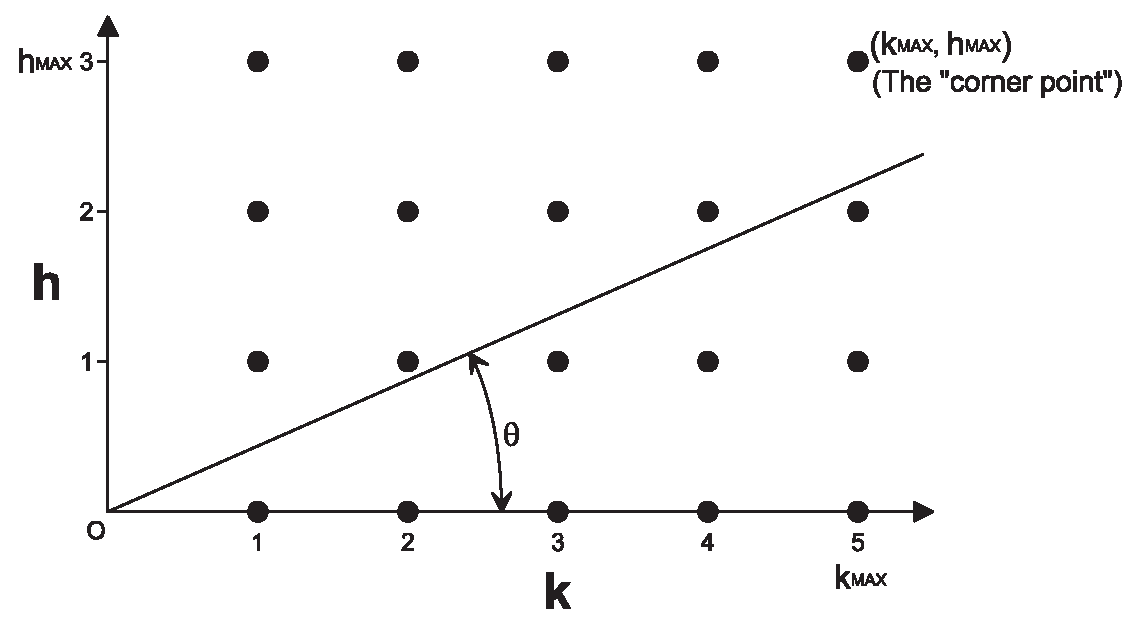
\includegraphics[width=4.6in]{c_rla1/farey01a.eps}
\caption{Graphical Interpretation Of Rational Numbers 
         $h/k$ That Can Be Formed With $h \leq h_{MAX}=3$, $k \leq k_{MAX}=5$}
\label{fig:crla1:slcr0:sfry0:00}
\end{figure}

From the graphical interpretation suggested by Fig. \ref{fig:crla1:slcr0:sfry0:00},
the following properties are intuitively clear.

\begin{itemize}
   \item The angle of a ray drawn from the origin to the point
         $(k,h)$ corresponding to the rational number $h/k$ is
         $\theta = tan^{-1} \; h/k$.

   \item Any integer lattice point on a line from 
         the origin drawn at the angle $\theta$
         has the value $h/k = tan \; \theta$.  All points corresponding
         to rational numbers with the same value will be on such a line,
         and thus form an equivalence class.

   \item A rational number $h/k$ is irreducible if and only if its corresponding
         point $(k,h)$ is ``directly'' visible from the origin with
         no intervening points.

   \item The Farey series of order $N$, $F_N$, can be 
         formed graphically by starting with the
         set of integer lattice points
         $(k,h): \; h \in \vworkintsetnonneg \wedge 1 \leq k \leq N$, 
         then sweeping
         a line extended from the origin, starting with 
         angle $\theta = 0$, through
         $0 \leq \theta < \pi{}/2$, and recording 
         in order each point directly visible from
         the origin.\footnote{Note that Fig. \ref{fig:crla1:slcr0:sfry0:00},
         because it illustrates the case when $h$ is constrained
         as well, does not show integer lattice points for
         $h > h_{MAX}$.  In principle, if the integer lattice shown
         in Fig. \ref{fig:crla1:slcr0:sfry0:00} were extended indefinitely
         ``upward'', every positive irreducible rational number with
         $k \leq k_{MAX} = 5$ could be found graphically.}
\end{itemize}

Fig. \ref{fig:crla1:slcr0:sfry0:01} illustrates the graphical construction method
of $F_5$.  Note that only integer lattice points which are directly
visible from the origin (with no intervening points) are selected.
(Fig. \ref{fig:crla1:slcr0:sfry0:01}, like Fig. \ref{fig:crla1:slcr0:sfry0:00},
shows the case of constrained $h$---the integer lattice should be
continued ``upward'' to construct the Farey series.)

\begin{figure}
\centering
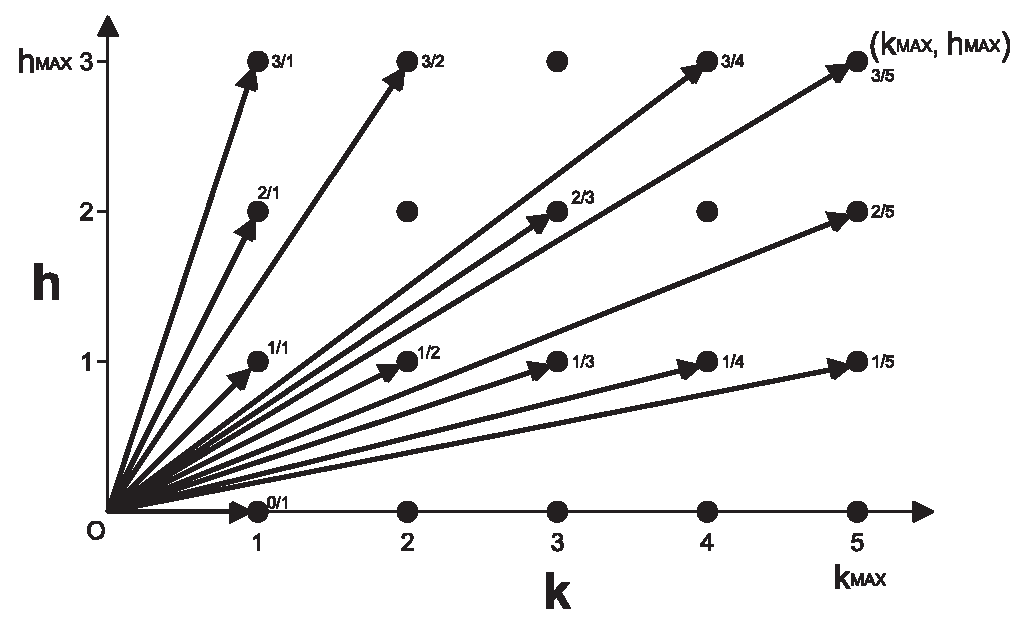
\includegraphics[width=4.6in]{c_rla1/farey01b.eps}
\caption{Graphical Interpretation Of Irreducible Rational Numbers 
         $h/k$ That Can Be Formed With $h \leq h_{MAX}=3$, $k \leq k_{MAX}=5$}
\label{fig:crla1:slcr0:sfry0:01}
\end{figure}

Note that Figures \ref{fig:crla1:slcr0:sfry0:00}
and \ref{fig:crla1:slcr0:sfry0:01} depict the case when
\emph{both} $h$ and $k$ are constrained (whereas the Farey series
constrains only $k$).

To give a compact notation, we denote the set of ascending irreducible
rational numbers that can be graphically formed
from Figures \ref{fig:crla1:slcr0:sfry0:00}
and \ref{fig:crla1:slcr0:sfry0:01} as  
$F_{k_{MAX}, h_{MAX}}$.  Using this notation, the graphical construction method
depicted in Figure \ref{fig:crla1:slcr0:sfry0:01} identifies $F_{5,3}$.

The ``corner point'' in Figures \ref{fig:crla1:slcr0:sfry0:00}
and \ref{fig:crla1:slcr0:sfry0:01} plays a special role:

\begin{itemize}
\item From 0/1 up through the corner point $h_{MAX}/k_{MAX}$,
      the terms are the terms of the Farey series of order
      $k_{MAX}$.
\item From $h_{MAX}/k_{MAX}$ up through $h_{MAX}/1$, the terms
      are the reverse-ordered reciprocals of the terms of the
      Farey series of order $h_{MAX}$.\footnote{This can be verified
      by transposing the $h$ and $k$ axes of the figures.}
\end{itemize}

As an example, $F_{5,3}$ identified graphically
is Figure \ref{fig:crla1:slcr0:sfry0:01} is

\begin{equation}
\label{eq:crla1:slcr0:sfry0:10}
F_5  = \left\{ {\frac{0}{1},\frac{1}{5},\frac{1}{4},
                \frac{1}{3},\frac{2}{5},\frac{1}{2},
                \frac{3}{5},\frac{2}{3},\frac{3}{4},
                \frac{1}{1},\frac{3}{2}, \frac{2}{1},
                \frac{3}{1} } \right\} .
\end{equation}

It can be seen by comparing (\ref{eq:crla1:slcr0:sfry0:10})
with (\ref{eq:crla1:slcr0:sfry0:eq0001c}) and 
(\ref{eq:crla1:slcr0:sfry0:eq0001e}) that the first seven terms of
(\ref{eq:crla1:slcr0:sfry0:10}) come from $F_5$ and the remaining
six terms are the reverse-ordered reciprocals of $F_3$ (although $F_3$
must be extended from Eq. \ref{eq:crla1:slcr0:sfry0:eq0001c}
into [1,2] to include 4/3 and 3/2).

The symmetry of Figures \ref{fig:crla1:slcr0:sfry0:00} and 
\ref{fig:crla1:slcr0:sfry0:01} with respect to the corner point
is important, because it means that finding best 
rational approximations for 
$r_I < h_{MAX}/k_{MAX}$ is the same problem as for 
$r_I > h_{MAX}/k_{MAX}$.  In the case of
$r_I < h_{MAX}/k_{MAX}$, the Farey series of order
$k_{MAX}$ is used, and in the case of
$r_I > h_{MAX}/k_{MAX}$ the Farey series of order
$h_{MAX}$ is used (but the reciprocals of the terms are
used, the order of the terms is reversed, and $1/r_I$ is used).  Thus, if we
know how to bracket $r_I < h_{MAX}/k_{MAX}$
in $F_{k_{MAX}}$, we can approach
the problem of $r_I > h_{MAX}/k_{MAX}$
through the inherent symmetry.


%%%%%%%%%%%%%%%%%%%%%%%%%%%%%%%%%%%%%%%%%%%%%%%%%%%%%%%%%%%%%%%%%%%%%%%%%%%%%%%
%%%%%%%%%%%%%%%%%%%%%%%%%%%%%%%%%%%%%%%%%%%%%%%%%%%%%%%%%%%%%%%%%%%%%%%%%%%%%%%
%%%%%%%%%%%%%%%%%%%%%%%%%%%%%%%%%%%%%%%%%%%%%%%%%%%%%%%%%%%%%%%%%%%%%%%%%%%%%%%

\subsection{The Continued Fraction Algorithm}

%Subsection Tag: cfr0
\label{crla1:slcr0:scfr0}

A \emph{finite simple continued fraction} is a fraction of the form

\begin{equation}
\label{eq:crla1:slcr0:scfr0:00}
a_0 + \cfrac{1}{a_1 + \cfrac{1}{a_2
    + \cfrac{1}{\;\;\;\;\;\;\;\;\;\;\;\;\;\;\ldots + \cfrac{1}{a_n}}}}
    =
    [a_0; a_1, a_2, \ldots , a_n] ,
\end{equation}

\noindent{}where $a_0 \in \vworkintsetnonneg$ and 
$a_i \in \vworkintsetpos$, $i > 0$.  Each integer
$a_i$ is called an \index{continued fraction!element}\emph{element} or
\index{continued fraction!partial quotient}\emph{partial quotient} 
of the continued fraction.
To ensure a unique representation, we require, except in the case of
the continued fraction representation of an integer,
that the final element $a_n$ not be equal
to 1.

Continued fractions are quite unwieldly to write and typeset,
and so a continued fraction in the form of (\ref{eq:crla1:slcr0:scfr0:00})
is written as $[a_0; a_1, a_2, \ldots , a_n]$.  Note that the
separator between $a_0$ and $a_1$ is a semicolon (`;'), and that all other
separators are commas (`,').  In some works, commas are used exclusively; and in
other works, the first element is $a_1$ rather than $a_0$.  Throughout this
work, the notational conventions illustrated in (\ref{eq:crla1:slcr0:scfr0:00}) are
followed.

Continued fractions can be either finite or infinite.

A finite continued fraction consists of a finite number of elements
$[a_0; a_1, a_2, \ldots , a_n]$.  It can be proved that 
every rational number corresponds to a unique
finite continued fraction\footnote{So long as the $a_n \neq 1$ convention
described earlier is followed.}, and that 
every finite continued fraction corresponds to a rational number. 

An infinite continued fraction consists of an infinite number
of elements $[a_0; a_1, a_2, \ldots]$.  Because every rational number
corresponds to a finite continued fraction, all irrational numbers have
infinite continued fraction representations.

In engineering work (and due to the general prevalence of computers
and calculators), any $r_I$ to be approximated has a known approximate
numerical value.  Even quantities that are known to be irrational (such
as $\pi$ or $\sqrt{2}$) have a numerical value known to a large number
of significant digits.  For this reason, only the numerical procedure for
obtaining the continued fraction representation of a rational number is
presented here (the symbolic procedure is not discussed).  Numerical values
are always rational (for example, 3.1415 is 31,415/10,000).

\index{continued fraction!convergent}
The \emph{kth order convergent} of a continued fraction
$[a_0; a_1, \ldots{}, a_n]$ is the irreducible rational number
corresponding to $[a_0; a_1, \ldots{}, a_k]$, $k \leq n$.
In other words, the $k$th order convergent is the irreducible rational number
corresponding to the first $k+1$ partial quotients of a 
continued fraction.\footnote{``$k+1$'' because the notational
numbering
for partial quotients starts at 0 rather than 1.} 

An $n$th order continued fraction $[a_0; a_1, \ldots{}, a_n]$
has $n+1$ convergents, $[a_0]$, 
$[a_0; a_1]$, \ldots{}, and $[a_0; a_1, \ldots{}, a_n]$.
We denote the $k$th order convergent as $s_k$, with numerator
$p_k$ and denominator $q_k$.

Without proof, we present the following algorithm, Algorithm 
\ref{alg:crla1:slcr0:scfr0:akgenalg}, for
determining the continued fraction representation (i.e. the partial
quotients) as well as the convergents of a non-negative
rational number $a/b$.

\begin{vworkalgorithmstatementpar}{Continued Fraction Representation and
                                   Convergents of 
                                   A Rational Number \mbox{\boldmath $a/b$}}
\label{alg:crla1:slcr0:scfr0:akgenalg}
\begin{alglvl0}
\item $k:=-1$.
\item $divisor_{-1} := a$.
\item $remainder_{-1} := b$.

\item Repeat

\begin{alglvl1}
\item $k := k + 1$.
\item $dividend_k := divisor_{k-1}$.
\item $divisor_k  := remainder_{k-1}$.
\item $a_k :=  dividend_k \; div \; divisor_k$.
\item $remainder_k := dividend_k \; mod \; divisor_k$.
\item If $k=0$, $p_0 = a_0$; else if $k=1$, $p_1 = a_0 a_1 + 1$; 
      else $p_i = a_i p_{i-1} + p_{i-2}$.
\item If $k=0$, $q_0 = 1$; else if $k=1$, $q_1 = a_1$; 
      else $q_i = a_i q_{i-1} + q_{i-2}$.
\end{alglvl1}

\item Until ($remainder_k = 0$).
\end{alglvl0}
\textbf{\emph{Note:}} The final $s_k = p_k / q_k$ is the irreducible
form of $a/b$.  For brevity, this is not proved here.
\end{vworkalgorithmstatementpar}
%\vworkalgorithmfooter{}
\begin{vworkexamplestatement}
\label{ex:crla1:slcr0:scfr0:01}
Find the continued fraction partial quotients and convergents of 
$67/29$.
\end{vworkexamplestatement}
\begin{vworkexampleparsection}{Solution} Table 
\ref{tbl:crla1:slcr0:scfr0:01} shows the application of 
Algorithm \ref{alg:crla1:slcr0:scfr0:akgenalg} to find the
continued fraction partial quotients and convergents of $67/29$.  From
Table \ref{tbl:crla1:slcr0:scfr0:01}, the continued fraction
representation of $67/29$ is $[2;3,4,2]$.

\begin{table}
\caption{Continued Fraction Partial Quotients and Convergents of $67/29$ (Example \ref{ex:crla1:slcr0:scfr0:01})}
\label{tbl:crla1:slcr0:scfr0:01}
\begin{center}
\begin{tabular}{|c|c|c|c|c|c|c|}
\hline
\small{Index} & \small{$dividend_k$}  & \small{$divisor_k$} & \small{$a_k$}   & \small{$remainder_k$} & \small{$p_k$} & \small{$q_k$} \\
\small{($k$)} &                       &                     &                 &                       &               &               \\
\hline
\hline
\small{-1}    & \small{N/A}           & \small{67}          & \small{N/A}     & \small{29}            & \small{N/A}   & \small{N/A}   \\
\hline
\small{0}     & \small{67}            & \small{29}          & \small{2}       & \small{9}             & \small{2}     & \small{1}     \\
\hline
\small{1}     & \small{29}            & \small{9}           & \small{3}       & \small{2}             & \small{7}     & \small{3}     \\
\hline
\small{2}     & \small{9}             & \small{2}           & \small{4}       & \small{1}             & \small{30}    & \small{13}    \\
\hline
\small{3}     & \small{2}             & \small{1}           & \small{2}       & \small{0}             & \small{67}    & \small{29}    \\
\hline
\end{tabular}
\end{center}
\end{table}
\end{vworkexampleparsection}
\vworkexamplefooter{}

Finally, we present without proof a theorem that indicates how to bracket
a rational number $a/b$ that is not in $F_{k_{MAX}}$ with its two neighbors
in $F_{k_{MAX}}$.

\begin{vworktheoremstatementpar}{Enclosing Neighbors Of \mbox{\boldmath $x \notin F_N$} 
                                 In \mbox{\boldmath $F_N$}}
\label{thm:crla1:slcr0:scfr0:cfenclosingneighbors}
For a non-negative rational
number $a/b$\footnote{It is not required that $a/b$ be irreducible in
order to apply this theorem.
For brevity, many properties of convergents were omitted; it is provable that 
the convergents formed by Algorithm \ref{alg:crla1:slcr0:scfr0:akgenalg}
will be identical for $a/b$ and $ia/ib$.} not in
$F_N$ which has a
continued fraction representation
$[a_0;a_1,a_2,\ldots{} ,a_n]$, the
highest-order convergent $s_k = p_k/q_k$ with $q_k \leq N$ is one
neighbor\footnote{By neighbors in $F_N$ we mean the rational numbers
in $F_N$ immediately to the left and immediately to the right
of $a/b$.}
to $a/b$ in $F_N$, and the other neighbor in
$F_N$ is\footnote{Theorem \ref{thm:crla1:slcr0:scfr0:cfenclosingneighbors}
is a somewhat stronger statement about best approximations
than Khinchin makes in \cite{bibref:b:KhinchinClassic}, Theorem 15.
We were not able to locate
this theorem or a proof in print,
but this theorem is understood within the number theory community.
It appears on the Web
page of David Eppstein \cite{bibref:i:davideppstein} in the form of a
`C'-language computer program,
\texttt{http://www.ics.uci.edu/\~{}{}eppstein/numth/frap.c}.
Although
Dr. Eppstein phrases the solution in terms of modifying
a partial quotient, his approach is equivalent to
(\ref{eq:crla1:slcr0:scfr0:thm:cfenclosingneighbors:01}).}

\begin{equation}
\label{eq:crla1:slcr0:scfr0:thm:cfenclosingneighbors:01}
\frac{{\displaystyle{\left\lfloor {\frac{{N - q_{k - 1} }}{{q_k }}} \right\rfloor}
 p_k  + p_{k - 1} }}{{\displaystyle{\left\lfloor {\frac{{N - q_{k - 1} }}{{q_k }}}
 \right\rfloor} q_k  + q_{k - 1} }}.
\end{equation}
\end{vworktheoremstatementpar}
\begin{vworktheoremproof}
Omitted, as it relies on material not presented for brevity.
\end{vworktheoremproof}
\vworktheoremfooter{}

Theorem \ref{thm:crla1:slcr0:scfr0:cfenclosingneighbors}
can also be applied to find the Farey neighbors of an $a/b$ already
in $F_{k_{MAX}}$.  If Algorithm \ref{alg:crla1:slcr0:scfr0:akgenalg}
is applied to $a/b$, (\ref{eq:crla1:slcr0:scfr0:thm:cfenclosingneighbors:01})
will provide one Farey neighbor, and 
(\ref{eq:crla1:slcr0:sfry0:thm:01:eq01}) through
(\ref{eq:crla1:slcr0:sfry0:thm:01:eq04}) can be used to provide the other
Farey neighbor.  (Again, for brevity, the mathematical basis for this
is not presented.)

Many constants $r_I$ to be approximated are engineering constants based
on measurements or arbitrary conventions, and so are known or accepted to
only a finite number of significant digits.  Such constants are always
rational, and 
Algorithm \ref{alg:crla1:slcr0:scfr0:akgenalg}
and
Theorem \ref{thm:crla1:slcr0:scfr0:cfenclosingneighbors}
can be applied with no special consideration.

Some constants, however, are irrational.  The question naturally arises
of how to be sure that one is using enough decimal digits
in applying 
Algorithm \ref{alg:crla1:slcr0:scfr0:akgenalg}
and
Theorem \ref{thm:crla1:slcr0:scfr0:cfenclosingneighbors}.
The easiest approach to apply in practice\footnote{\emph{In practice}
because some theoretical results may be possible as far as how
many significant digits are always adequate or as far as other
criteria, but the approach taken here is the easiest practical one.}
is to confine the quantity of interest by an inequality and to be
sure that the results are the same at both boundaries
of the inequality.

For example, $\pi$ is a transcendental constant, so has a non-terminating
decimal representation.  $\pi$ to several digits (truncated at the
end) is 3.1415926535.  It follows that

\begin{equation}
\label{eq:crla1:slcr0:scfr0:30}
3.1415926535 < \pi < 3.1415926536
\end{equation}  

For compact notation, we denote the left limit as $r_{LEFT}$ and the
right limit by $r_{RIGHT}$.  We also make the observation that in some
applications, the interval is closed rather than open.\footnote{This depends
on how much is known about $r_I$---for example, we know that $\pi$ is irrational and
can't be equal to any rational number, but we
may not know this about other $r_I$ of interest.}  In the more
general case, $r_I$ is confined by:

\begin{equation}
\label{eq:crla1:slcr0:scfr0:30b}
r_{LEFT} \leq r_I < r_{RIGHT} .
\end{equation}  

With the the $r_I$ of interest confined as suggested in 
(\ref{eq:crla1:slcr0:scfr0:30b}), there are two easy approaches
to decide if the Farey neighbors of $r_I$ can be determined with
the information available.

\begin{enumerate}
\item \emph{Easier:} Locate the Farey neighbors $h_L/k_L$ and $h_R/k_R$ of
      $r_{LEFT}$, then numerically determine whether 
      $h_L/k_L \leq r_{RIGHT} \leq h_R/k_R$.
\item \emph{Harder:} Determine whether $r_{LEFT}$ and $r_{RIGHT}$ have the
      same convergents up through $p_k/q_k$ with $q_k \leq N$.  If so,
      $r_{LEFT}$ and $r_{RIGHT}$ have the same Farey neighbors.
\end{enumerate}

\noindent{}If 
Algorithm \ref{alg:crla1:slcr0:scfr0:akgenalg}
and
Theorem \ref{thm:crla1:slcr0:scfr0:cfenclosingneighbors} are
applied with 31415926535/10000000000 and 31415926536/10000000000 
separately and yield the same rational numbers $h_L/k_L$ and $h_R/k_R$ as 
left and right neighbors, then

\begin{equation}
\label{eq:crla1:slcr0:scfr0:31}
\frac{h_L}{k_L} < 3.1415926535 < \pi < 3.1415926536 < \frac{h_R}{k_R}
\end{equation}  

\noindent{}and it is thus confirmed that $h_L/k_L$ and $h_R/k_R$ are the left
and right neighbors of $\pi$ in the Farey series of interest.

Several examples follow which illustrate the technique and various special
cases.

\begin{vworkexamplestatement}
\label{ex:crla1:slcr0:scfr0:10}
Find the best rational approximation to $1/e$ in $F_{65535}$.
\end{vworkexamplestatement}
\begin{vworkexampleparsection}{Solution} Note that $e$ is irrational, implying
that $1/e$ is also irrational, thus a bounding technique might best be used
to ensure finding the correct Farey neighbors.  Using an ordinary scientific pocket
calculator, the displayed value of $e^{-1}$ is approximately 0.367879441171.
Allowing for some possible imprecision in the last digit\footnote{The guess at 
how accurate a calculator is likely to be is subjective.}, it is fairly safe to assume that

\begin{equation}
\label{eq:ex:crla1:slcr0:scfr0:10:01}
\frac{367879441170}{1000000000000} < \frac{1}{e} < \frac{367879441172}{1000000000000} .
\end{equation}

Table \ref{tbl:crla1:slcr0:scfr0:10a} shows the application of 
Algorithm \ref{alg:crla1:slcr0:scfr0:akgenalg} to find the
continued fraction partial quotients of the left inequality
limit, and Table Table \ref{tbl:crla1:slcr0:scfr0:10b} shows the
calculation of the convergents.  (The tables are separated due to typesetting
limitations---the partial quotients and convergents would normally be tabulated
together.)

\begin{table}
\caption{Continued Fraction Partial Quotients of $367,879,441,170/1,000,000,000,000$ (Example \ref{ex:crla1:slcr0:scfr0:10})}
\label{tbl:crla1:slcr0:scfr0:10a}
\begin{center}
\begin{tabular}{|c|c|c|c|c|}
\hline
\small{Index} & \small{$dividend_k$}      & \small{$divisor_k$}       & \small{$a_k$}   & \small{$remainder_k$}     \\
\small{($k$)} &                           &                           &                 &                           \\
\hline
\hline
\small{-1}    & \small{N/A}               & \small{367,879,441,170}   & \small{N/A}     & \small{1,000,000,000,000} \\
\hline
\small{0}     & \small{367,879,441,170}   & \small{1,000,000,000,000} & \small{0}       & \small{367,879,441,170}   \\
\hline
\small{1}     & \small{1,000,000,000,000} & \small{367,879,441,170}   & \small{2}       & \small{264,241,117,660}   \\
\hline
\small{2}     & \small{367,879,441,170}   & \small{264,241,117,660}   & \small{1}       & \small{103,638,323,510}   \\
\hline
\small{3}     & \small{264,241,117,660}   & \small{103,638,323,510}   & \small{2}       & \small{56,964,470,640}    \\
\hline
\small{4}     & \small{103,638,323,510}   & \small{56,964,470,640}    & \small{1}       & \small{46,673,852,870}    \\
\hline
\small{5}     & \small{56,964,470,640}    & \small{46,673,852,870}    & \small{1}       & \small{10,290,617,770}    \\
\hline
\small{6}     & \small{46,673,852,870}    & \small{10,290,617,770}    & \small{4}       & \small{5,511,381,790}     \\
\hline
\small{7}     & \small{10,290,617,770}    & \small{5,511,381,790}     & \small{1}       & \small{4,779,235,980}     \\
\hline
\small{8}     & \small{5,511,381,790}     & \small{4,779,235,980}     & \small{1}       & \small{732,145,810}       \\
\hline
\small{9}     & \small{4,779,235,980}     & \small{732,145,810}       & \small{6}       & \small{386,361,120}       \\
\hline
\small{10}    & \small{732,145,810}       & \small{386,361,120}       & \small{1}       & \small{345,784,690}       \\
\hline
\small{11}    & \small{386,361,120}       & \small{345,784,690}       & \small{1}       & \small{40,576,430}        \\
\hline
\small{12}    & \small{345,784,690}       & \small{40,576,430}        & \small{8}       & \small{21,173,250}        \\
\hline
\small{13}    & \small{40,576,430}       & \small{21,173,250}         & \small{1}       & \small{19,403,180}        \\
\hline
\small{14}    & \small{21,173,250}       & \small{19,403,180}         & \small{1}       & \small{1,770,070}         \\
\hline
\small{15}    & \small{19,403,180}       & \small{1,770,070}          & \small{10}      & \small{1,702,480}         \\
\hline
\small{16}    & \small{1,770,070}        & \small{1,702,480}          & \small{1}       & \small{67,590}            \\
\hline
\small{17}    & \small{1,702,480}        & \small{67,590}             & \small{25}      & \small{12,730}            \\
\hline
\small{18}    & \small{67,590}           & \small{12,730}             & \small{5}       & \small{3,940}             \\
\hline
\small{19}    & \small{12,730}           & \small{3,940}              & \small{3}       & \small{910}               \\
\hline
\small{20}    & \small{3,940}            & \small{910}                & \small{4}       & \small{300}               \\
\hline
\small{21}    & \small{910}              & \small{300}                & \small{3}       & \small{10}                \\
\hline
\small{22}    & \small{300}              & \small{10}                 & \small{30}      & \small{0}                 \\
\hline
\end{tabular}
\end{center}
\end{table}

\begin{table}
\caption{Continued Fraction Convergents of $367,879,441,170/1,000,000,000,000$ (Example \ref{ex:crla1:slcr0:scfr0:10})}
\label{tbl:crla1:slcr0:scfr0:10b}
\begin{center}
\begin{tabular}{|c|c|c|c|}
\hline
\small{Index} & \small{$a_k$} & \small{$p_k$}           & \small{$q_k$}            \\
\small{($k$)} &               &                         &                          \\
\hline
\hline
\small{-1}    & \small{N/A}   & \small{N/A}             & \small{N/A}              \\
\hline
\small{0}     & \small{0}     & \small{0}               & \small{1}                \\
\hline
\small{1}     & \small{2}     & \small{1}               & \small{2}                \\
\hline
\small{2}     & \small{1}     & \small{1}               & \small{3}                \\
\hline
\small{3}     & \small{2}     & \small{3}               & \small{8}                \\
\hline
\small{4}     & \small{1}     & \small{4}               & \small{11}               \\
\hline
\small{5}     & \small{1}     & \small{7}               & \small{19}               \\
\hline
\small{6}     & \small{4}     & \small{32}              & \small{87}               \\
\hline
\small{7}     & \small{1}     & \small{39}              & \small{106}              \\
\hline
\small{8}     & \small{1}     & \small{71}              & \small{193}              \\
\hline
\small{9}     & \small{6}     & \small{465}             & \small{1,264}            \\
\hline
\small{10}    & \small{1}     & \small{536}             & \small{1,457}            \\
\hline
\small{11}    & \small{1}     & \small{1,001}           & \small{2,721}            \\
\hline
\small{12}    & \small{8}     & \small{8,544}           & \small{23,225}           \\
\hline
\small{13}    & \small{1}     & \small{9,545}           & \small{25,946}           \\
\hline
\small{14}    & \small{1}     & \small{18,089}          & \small{49,171}          \\
\hline
\small{15}    & \small{10}    & \small{190,435}         & \small{517,656}         \\
\hline
\small{16}    & \small{1}     & \small{208,524}         & \small{566,827}          \\
\hline
\small{17}    & \small{25}    & \small{5,403,535}       & \small{14,688,331}       \\
\hline
\small{18}    & \small{5}     & \small{27,226,199}      & \small{74,008,482}       \\
\hline
\small{19}    & \small{3}     & \small{87,082,132}      & \small{236,713,777}      \\
\hline
\small{20}    & \small{4}     & \small{375,554,727}     & \small{1,020,863,590}    \\
\hline
\small{21}    & \small{3}     & \small{1,213,746,313}   & \small{3,299,304,547}    \\
\hline
\small{22}    & \small{30}    & \small{36,787,944,117}  & \small{100,000,000,000}  \\
\hline
\end{tabular}
\end{center}
\end{table}

Note that since we are finding best rational approximations
in $F_{65535}$, Theorem \ref{thm:crla1:slcr0:scfr0:cfenclosingneighbors}
requires only that we carry the tabular procedure of 
Algorithm \ref{alg:crla1:slcr0:scfr0:akgenalg} out until
$q_k \geq 65535$ ($k=15$ in this example).

By
Theorem \ref{thm:crla1:slcr0:scfr0:cfenclosingneighbors}
and
Table \ref{tbl:crla1:slcr0:scfr0:10b}, one Farey neighbor
to the left inequality limit is $p_{14}/q_{14} = 18,089/49,171$.
The other Farey neighbor is given by 
(\ref{eq:crla1:slcr0:scfr0:thm:cfenclosingneighbors:01}), with the calculation
detailed below.

\begin{equation}
\label{eq:ex:crla1:slcr0:scfr0:10:50a}
\frac{{\displaystyle{\left\lfloor {\frac{{N - q_{k - 1} }}{{q_k }}} \right\rfloor}
 p_k  + p_{k - 1} }}{{\displaystyle{\left\lfloor {\frac{{N - q_{k - 1} }}{{q_k }}}
 \right\rfloor} q_k  + q_{k - 1} }}.
\end{equation}

\begin{equation}
\label{eq:ex:crla1:slcr0:scfr0:10:50b}
= \frac{{\displaystyle{\left\lfloor {\frac{{65535 - q_{13} }}{{q_{14} }}} \right\rfloor}
 p_{14}  + p_{13} }}{{\displaystyle{\left\lfloor {\frac{{65535 - q_{13} }}{{q_{14} }}}
 \right\rfloor} q_{14}  + q_{13} }}.
\end{equation}

\begin{equation}
\label{eq:ex:crla1:slcr0:scfr0:10:50c}
= \frac{{\displaystyle{\left\lfloor {\frac{{65535 - 25946 }}{{49171 }}} \right\rfloor}
 18089  + 9545 }}{{\displaystyle{\left\lfloor {\frac{{65535 - 25946 }}{{49171 }}}
 \right\rfloor} 49171  + 25946 }}.
\end{equation}

\begin{equation}
\label{eq:ex:crla1:slcr0:scfr0:10:50d}
= \frac{9545}{25946}
\end{equation}

It can be verified by cross-multiplication that $9545/25946 > 18089/49171$, therefore

\begin{equation}
\label{eq:ex:crla1:slcr0:scfr0:10:50e}
\frac{18089}{49171} < 0.367879441170 < \frac{9545}{25946} .
\end{equation}

A similar tabulation procedure carried out with 
the right inequality limit (0.367879441172), not reproduced here for brevity,
verifies that it has the same convergents up through $s_{15}$ as the left
inequality limit.  Therefore it has the same Farey neighbors in $F_{65535}$
as the left limit, and it is established that

\begin{equation}
\label{eq:ex:crla1:slcr0:scfr0:10:50f}
\frac{18089}{49171} < 0.367879441170 < \frac{1}{e} < 0.367879441172 < \frac{9545}{25946} .
\end{equation}

It can be verified numerically that 18089/49171 and 9545/25946 are both \emph{very}
close approximations to $1/e$ (with differences on the order of a couple parts per
\emph{billion}).
\end{vworkexampleparsection}
%\vworkexamplefooter{}

\begin{vworkexamplestatement}
\label{ex:crla1:slcr0:scfr0:11}
Find the enclosing neighbors to $8/43$ in $F_{65535}$.
\end{vworkexamplestatement}
\begin{vworkexampleparsection}{Solution} As hinted earlier,
since $8/43 \in F_{65535}$, we can simply treat 8/43 as a number very close to 8/43
so that the convergent after $s_k = 8/43$ has a larger denominator than 65535 (the details
of why and how this works are omitted for brevity).

\begin{table}
\caption{Continued Fraction Partial Quotients and Convergents of $8/43$ (Example \ref{ex:crla1:slcr0:scfr0:11})}
\label{tbl:crla1:slcr0:scfr0:11a}
\begin{center}
\begin{tabular}{|c|c|c|c|c|c|c|}
\hline
\small{Index} & \small{$dividend_k$} & \small{$divisor_k$} & \small{$a_k$} & \small{$remainder_k$} & \small{$p_k$} & \small{$q_k$} \\
\small{($k$)} &                      &                     &               &                       &               &               \\
\hline
\hline
\small{-1}    & \small{N/A}          & \small{8}           & \small{N/A}   & \small{43}            & \small{N/A}   & \small{N/A}   \\
\hline
\small{0}     & \small{8}            & \small{43}          & \small{0}     & \small{8}             & \small{0}     & \small{1}     \\
\hline
\small{1}     & \small{43}           & \small{8}           & \small{5}     & \small{3}             & \small{1}     & \small{5}     \\
\hline
\small{2}     & \small{8}            & \small{3}           & \small{2}     & \small{2}             & \small{2}     & \small{11}    \\
\hline
\small{3}     & \small{3}            & \small{2}           & \small{1}     & \small{1}             & \small{3}     & \small{16}    \\
\hline
\small{4}     & \small{2}            & \small{1}           & \small{2}     & \small{0}             & \small{8}     & \small{43}    \\
\hline
\end{tabular}
\end{center}
\end{table}

Table \ref{tbl:crla1:slcr0:scfr0:11a} shows the
application of 
Algorithm \ref{alg:crla1:slcr0:scfr0:akgenalg}
to determine the partial quotients and convergents of 8/43.

(\ref{eq:crla1:slcr0:scfr0:thm:cfenclosingneighbors:01}) can then be applied
to find a Farey neighbor of 8/43, with the calculation
detailed below.\footnote{Whether the left or right Farey neighbor is found depends on
whether the final convergent has $k$ even or $k$ odd.  The explanation is beyond the scope here.}

\begin{equation}
\label{eq:ex:crla1:slcr0:scfr0:11:50a}
\frac{{\displaystyle{\left\lfloor {\frac{{N - q_{k - 1} }}{{q_k }}} \right\rfloor}
 p_k  + p_{k - 1} }}{{\displaystyle{\left\lfloor {\frac{{N - q_{k - 1} }}{{q_k }}}
 \right\rfloor} q_k  + q_{k - 1} }}.
\end{equation}

\begin{equation}
\label{eq:ex:crla1:slcr0:scfr0:11:50b}
= \frac{{\displaystyle{\left\lfloor {\frac{{65535 - q_{3} }}{{q_{4} }}} \right\rfloor}
 p_{4}  + p_{3} }}{{\displaystyle{\left\lfloor {\frac{{65535 - q_{3} }}{{q_{4} }}}
 \right\rfloor} q_{4}  + q_{3} }}.
\end{equation}

\begin{equation}
\label{eq:ex:crla1:slcr0:scfr0:11:50c}
= \frac{{\displaystyle{\left\lfloor {\frac{{65535 - 16 }}{{43 }}} \right\rfloor}
 8  + 3 }}{{\displaystyle{\left\lfloor {\frac{{65535 - 16 }}{{43 }}}
 \right\rfloor} 43  + 16 }}.
\end{equation}

\begin{equation}
\label{eq:ex:crla1:slcr0:scfr0:11:50d}
= \frac{12187}{65505}
\end{equation}

It can be verified by cross-multiplication that (\ref{eq:ex:crla1:slcr0:scfr0:11:50d})
is the right Farey neighbor of 8/43.  As two consecutive
terms in $F_{65535}$ are now known, (\ref{eq:crla1:slcr0:sfry0:thm:01:eq03})
and (\ref{eq:crla1:slcr0:sfry0:thm:01:eq04}) can be applied to find the left Farey
neighbor, as shown below.

\begin{equation}
\label{eq:ex:crla1:slcr0:scfr0:11:51}
h_j  = \left\lfloor {\frac{{k_{j + 2}  + N}}{{k_{j + 1} }}} 
\right\rfloor h_{j + 1}  - h_{j + 2}
\end{equation}

\begin{equation}
\label{eq:ex:crla1:slcr0:scfr0:11:52}
= \left\lfloor {\frac{{65505  + 65535}}{{43 }}} 
\right\rfloor 8  - 12187 = 12189
\end{equation}

\begin{equation}
\label{eq:ex:crla1:slcr0:scfr0:11:55}
k_j  = \left\lfloor {\frac{{k_{j + 2}  + N}}{{k_{j + 1} }}} 
\right\rfloor k_{j + 1}  - k_{j + 2}
\end{equation}

\begin{equation}
\label{eq:ex:crla1:slcr0:scfr0:11:56}
= \left\lfloor {\frac{{65505  + 65535}}{{43 }}} 
\right\rfloor 43  - 65505 = 65516
\end{equation}

Thus, 12189/65516 is the left neighbor to 8/43 in $F_{65535}$.
\end{vworkexampleparsection}
%\vworkexamplefooter{}

\begin{vworkexamplestatement}
\label{ex:crla1:slcr0:scfr0:12}
Create assembly-language code to form an approximation 
to multiplication by $\pi$ that 
can be implemented using a \texttt{MUL} instruction followed by
a \texttt{DIV} instruction on the Freescale CPU08 core.  Assume that:
\begin{itemize}
\item The input is an 8-bit unsigned integer, passed in the accumulator.
\item The output is an 8-bit unsigned integer, returned in the accumulator.
\item The code is ``in-line'' (i.e. not a subroutine), and the code is free to modify
      any processor registers or flags.
\item Input data that is too large should cause the output to be clipped at 255 (the
      maximum value for an unsigned byte).
\end{itemize}
\end{vworkexamplestatement}
\begin{vworkexampleparsection}{Solution} $\pi$ is transcendental, and based
on the first several digits, can be bounded by

\begin{equation}
\label{eq:ex:crla1:slcr0:scfr0:12:01}
3.1415926535 < \pi < 3.1415926536 .
\end{equation}  

We first note that, due to the charactertistics of the CPU08, 
$h_{MAX} = 255$ and $k_{MAX} = 255$.  We are thus operating in
$F_{255, 255}$, with a corner point of $h/k = 255/255 = 1$.
$\pi > 1$, so we are operating along the top side of Figures
\ref{fig:crla1:slcr0:sfry0:00} and \ref{fig:crla1:slcr0:sfry0:01}
(pages \pageref{fig:crla1:slcr0:sfry0:00} and \pageref{fig:crla1:slcr0:sfry0:01}).
In this region above the corner point, the numerator rather than the denominator
is constrained.

As discussed earlier, to obtain best rational approximations above the corner point,
we may transpose the problem to that of obtaining best rational approximations
to $1/\pi$ in $F_{h_{MAX}}$ (rather than $F_{k_{MAX}}$---it is coincidental in this
case that $h_{MAX} = k_{MAX}$).

Algorithm \ref{alg:crla1:slcr0:scfr0:akgenalg} requires only a rational number as a starting
point, so it is most expedient to invert the terms of 
(\ref{eq:ex:crla1:slcr0:scfr0:12:01}) to yield

\begin{equation}
\label{eq:ex:crla1:slcr0:scfr0:12:02}
\frac{10000000000}{31415926536} 
< 
\frac{1}{\pi} 
< 
\frac{10000000000}{31415926535} .
\end{equation}

\begin{table}
\caption{Continued Fraction Partial Quotients and Convergents of $10000000000/31415926536$ (Example \ref{ex:crla1:slcr0:scfr0:12})}
\label{tbl:ex:crla1:slcr0:scfr0:12a}
\begin{center}
\begin{tabular}{|c|c|c|c|c|c|c|}
\hline
\small{$k$} & \small{$dividend_k$}  & \small{$divisor_k$}   & \small{$a_k$} & \small{$remainder_k$}    & \small{$p_k$}            & \small{$q_k$}            \\
\hline
\hline
\small{-1}   & \small{N/A}            & \small{10,000,000,000} & \small{N/A}    & \small{31,415,926,536}    & \small{N/A}               & \small{N/A}               \\
\hline
\small{0}    & \small{10,000,000,000} & \small{31,415,926,536} & \small{0}      & \small{10,000,000,000}    & \small{0}                 & \small{1}                 \\
\hline
\small{1}    & \small{31,415,926,536} & \small{10,000,000,000} & \small{3}      & \small{1,415,926,536}     & \small{1}                 & \small{3}                 \\
\hline
\small{2}    & \small{10,000,000,000} & \small{1,415,926,536}  & \small{7}      & \small{88,514,248}        & \small{7}                 & \small{22}                \\
\hline
\small{3}    & \small{1,415,926,536}  & \small{88,514,248}     & \small{15}     & \small{88,212,816}        & \small{106}               & \small{333}               \\
\hline
\multicolumn{7}{|c|}{\small{It isn't necessary to carry Algorithm \ref{alg:crla1:slcr0:scfr0:akgenalg}}}  \\ 
\multicolumn{7}{|c|}{\small{any further, as it has been established that $s_2 = 7/22$ is the last}}       \\
\multicolumn{7}{|c|}{\small{convergent with $q_k \leq 255$.}}                                             \\
\hline
\end{tabular}
\end{center}
\end{table}

Table \ref{tbl:ex:crla1:slcr0:scfr0:12a} shows the application of 
Algorithm \ref{alg:crla1:slcr0:scfr0:akgenalg} to obtain the partial
quotients and convergents of $10000000000/31415926536$.  Note that it is not
necessary to carry out the algorithm any further than establishing the
highest-order convergent with $q_k \leq h_{MAX} = 255$.

By Theorem \ref{thm:crla1:slcr0:scfr0:cfenclosingneighbors} 7/22 is either
the left or right Farey neighbor to 10000000000/31415926536.  Numerically,
it can be verified that 7/22 is the left Farey neighbor.

The right Farey neighbor is given by 
(\ref{eq:crla1:slcr0:scfr0:thm:cfenclosingneighbors:01}), with the calculation
detailed below.

\begin{equation}
\label{eq:ex:crla1:slcr0:scfr0:12:10a}
\frac{{\displaystyle{\left\lfloor {\frac{{N - q_{k - 1} }}{{q_k }}} \right\rfloor}
 p_k  + p_{k - 1} }}{{\displaystyle{\left\lfloor {\frac{{N - q_{k - 1} }}{{q_k }}}
 \right\rfloor} q_k  + q_{k - 1} }}
\end{equation}

\begin{equation}
\label{eq:ex:crla1:slcr0:scfr0:12:10b}
= \frac{{\displaystyle{\left\lfloor {\frac{{255 - q_{1} }}{{q_{2} }}} \right\rfloor}
 p_{2}  + p_{1} }}{{\displaystyle{\left\lfloor {\frac{{255 - q_{1} }}{{q_{2} }}}
 \right\rfloor} q_{2}  + q_{1} }}
\end{equation}

\begin{equation}
\label{eq:ex:crla1:slcr0:scfr0:12:10c}
= \frac{{\displaystyle{\left\lfloor {\frac{{255 - 3 }}{{22 }}} \right\rfloor}
 7  + 1 }}{{\displaystyle{\left\lfloor {\frac{{255 - 3 }}{{22 }}}
 \right\rfloor} 22  + 3 }}
\end{equation}

\begin{equation}
\label{eq:ex:crla1:slcr0:scfr0:12:10d}
= \frac{78}{245}
\end{equation}

We have shown that

\begin{equation}
\label{eq:ex:crla1:slcr0:scfr0:12:20}
\frac{7}{22}
<
\frac{10000000000}{31415926536}
<
\frac{78}{245} .
\end{equation}

However, we can't bound $1/\pi$ without checking whether the right
limit of 
(\ref{eq:ex:crla1:slcr0:scfr0:12:02}) falls between 
7/22 and 78/245.  It is easy to verify numerically that this is the case.
(If this were not the case, Eq. \ref{eq:ex:crla1:slcr0:scfr0:12:02} should
be rephrased using more digits of $\pi$.)

It is then known that:

\begin{equation}
\label{eq:ex:crla1:slcr0:scfr0:12:21}
\frac{7}{22}
<
\frac{10000000000}{31415926536}
<
\frac{1}{\pi}
<
\frac{10000000000}{31415926536}
<
\frac{78}{245} .
\end{equation}

In order to convert (\ref{eq:ex:crla1:slcr0:scfr0:12:21})
to a form involving constrained $h_{MAX}$ and $\pi$, we must 
invert the terms and reverse the order of the inequality.

\begin{equation}
\label{eq:ex:crla1:slcr0:scfr0:12:22}
\frac{245}{78} 
<
\frac{31415926536}{10000000000}
<
\pi
<
\frac{31415926535}{10000000000}
<
\frac{22}{7}
\end{equation}

It has thus been shown that, subject to the constraints
$h \leq 255$ and $k \leq 255$, the surrounding rational approximations
to $\pi$ are 245/78 and 22/7.  Since 245/78 is the better approximation, that
is used for the assembly-language code (Figure \ref{fig:ex:crla1:slcr0:scfr0:12:10}).

\begin{figure}
\begin{verbatim}
          ;Assume input argument in accumulator.
          cmp  #82
          bhs  toobig  ;Input argument is 82 or larger.  Must
                       ;clip or will overflow MUL and/or DIV.
          ldx  #245    ;Set up to multiply A by 245.
          mul          ;X:A now contains MSB:LSB multiplication
                       ;result.
          pshx         ;Push/pull best way to get X into H
          pulh         ;to set up for division.
          ldx  #78     ;78 is divisor.
          div          ;Do the division.  Result guaranteed to
                       ;be in range as divisor could be no
                       ;larger than 19,845 before division.
          bra  theend  ;Branch around clip.
toobig:   lda  #255    ;Load "clip" value.
theend:
          ;Output result now in accumulator.
\end{verbatim}
\caption{Freescale CPU08 Code to Approximate $\pi$ (Example \ref{ex:crla1:slcr0:scfr0:12})}
\label{fig:ex:crla1:slcr0:scfr0:12:10}
\end{figure}

In order to ``clip'' so that any input arguments too large result in an output of 255,
it is necessary to determine which input arguments will be problematic.  This is done
in the inequality below, and the result appears in the assembly-language code of
(Figure \ref{fig:ex:crla1:slcr0:scfr0:12:10}).

\begin{equation}
\label{eq:ex:crla1:slcr0:scfr0:12:23}
\left({\left\lfloor{\frac{245 x}{78}}\right\rfloor 
\geq 256}\right) 
\longrightarrow \left({x \geq 82}\right)
\end{equation}
\end{vworkexampleparsection}
\vworkexamplefooter{}


%%%%%%%%%%%%%%%%%%%%%%%%%%%%%%%%%%%%%%%%%%%%%%%%%%%%%%%%%%%%%%%%%%%%%%%%%%%%%%%
%%%%%%%%%%%%%%%%%%%%%%%%%%%%%%%%%%%%%%%%%%%%%%%%%%%%%%%%%%%%%%%%%%%%%%%%%%%%%%%
%%%%%%%%%%%%%%%%%%%%%%%%%%%%%%%%%%%%%%%%%%%%%%%%%%%%%%%%%%%%%%%%%%%%%%%%%%%%%%%

\section[Choosing $r_A = h/2^q \approx r_I$]
        {Choosing \mbox{\boldmath $r_A = h/2^q \approx r_I$}}

%Section Tag: lcr0
\label{crla1:slcr1}


%%%%%%%%%%%%%%%%%%%%%%%%%%%%%%%%%%%%%%%%%%%%%%%%%%%%%%%%%%%%%%%%%%%%%%%%%%%%%%%
%%%%%%%%%%%%%%%%%%%%%%%%%%%%%%%%%%%%%%%%%%%%%%%%%%%%%%%%%%%%%%%%%%%%%%%%%%%%%%%
%%%%%%%%%%%%%%%%%%%%%%%%%%%%%%%%%%%%%%%%%%%%%%%%%%%%%%%%%%%%%%%%%%%%%%%%%%%%%%%

\section[Choosing $r_A = 2^p/k \approx r_I$]
        {Choosing \mbox{\boldmath $r_A = 2^p/k \approx r_I$}}

%Section Tag: lcr0
\label{crla1:slcr2}


%%%%%%%%%%%%%%%%%%%%%%%%%%%%%%%%%%%%%%%%%%%%%%%%%%%%%%%%%%%%%%%%%%%%%%%%%%%%%%%
%%%%%%%%%%%%%%%%%%%%%%%%%%%%%%%%%%%%%%%%%%%%%%%%%%%%%%%%%%%%%%%%%%%%%%%%%%%%%%%
%%%%%%%%%%%%%%%%%%%%%%%%%%%%%%%%%%%%%%%%%%%%%%%%%%%%%%%%%%%%%%%%%%%%%%%%%%%%%%%

\section{End-to-End Approximation Error}

%Section Tag: ete0
\label{crla1:sete2}

%
%%%%%%%%%%%%%%%%%%%%%%%%%%%%%%%%%%%%%%%%%%%%%%%%%%%%%%%%%%%%%%%%%%%%%%%%%%%
%
%\noindent\begin{figure}[!b]
%\noindent\rule[-0.25in]{\textwidth}{1pt}
%\begin{tiny}
%\begin{verbatim}
%$RCSfile: c_rla1.tex,v $
%$Source: /home/dashley/cvsrep/uculib01/uculib01/doc/manual/c_rla1/c_rla1.tex,v $
%$Revision: 1.11 $
%$Author: dashley $
%$Date: 2010/01/28 21:18:33 $
%\end{verbatim}
%\end{tiny}
%\noindent\rule[0.25in]{\textwidth}{1pt}
%\end{figure}
%
%%%%%%%%%%%%%%%%%%%%%%%%%%%%%%%%%%%%%%%%%%%%%%%%%%%%%%%%%%%%%%%%%%%%%%%%%%%%%%%
%% $Log: c_rla1.tex,v $
%% Revision 1.11  2010/01/28 21:18:33  dashley
%% a)Chapter start quotes removed.
%% b)Aesthetic comment line added at the bottom of most files.
%%
%% Revision 1.10  2007/10/01 14:20:01  dtashley
%% Example completed.
%%
%% Revision 1.9  2007/10/01 02:02:49  dtashley
%% Edits.
%%
%% Revision 1.8  2007/09/30 21:59:51  dtashley
%% Edits.
%%
%% Revision 1.7  2007/09/29 04:58:42  dtashley
%% Edits.
%%
%% Revision 1.6  2007/09/29 03:15:56  dtashley
%% Edits.
%%
%% Revision 1.5  2007/09/28 19:59:55  dtashley
%% Edits.
%%
%% Revision 1.4  2007/09/28 04:59:49  dtashley
%% Edits.
%%
%% Revision 1.3  2007/09/27 22:54:33  dtashley
%% Edits.
%%
%% Revision 1.2  2007/09/27 21:44:22  dtashley
%% Edits.
%%
%% Revision 1.1  2007/09/27 15:23:31  dtashley
%% Initial checkin.
%%
%%End of $RCSfile: c_rla1.tex,v $.
%%%%%%%%%%%%%%%%%%%%%%%%%%%%%%%%%%%%%%%%%%%%%%%%%%%%%%%%%%%%%%%%%%%%%%%%%%%%%%%



%Part: Developer Information
%\part{Developer Information}

%Chapter: UCULIB Build Procedures
%%$Header: /home/dashley/cvsrep/uculib01/uculib01/doc/manual/c_bpc0/c_bpc0.tex,v 1.3 2010/01/28 21:18:32 dashley Exp $

\chapter{\emph{\productbasenameshort{}} Build Procedures}        
\label{cbpc0}

%%%%%%%%%%%%%%%%%%%%%%%%%%%%%%%%%%%%%%%%%%%%%%%%%%%%%%%%%%%%%%%%%%%%%%%%%%%%%%%
%%%%%%%%%%%%%%%%%%%%%%%%%%%%%%%%%%%%%%%%%%%%%%%%%%%%%%%%%%%%%%%%%%%%%%%%%%%%%%%
%%%%%%%%%%%%%%%%%%%%%%%%%%%%%%%%%%%%%%%%%%%%%%%%%%%%%%%%%%%%%%%%%%%%%%%%%%%%%%%
\section{Introduction and Overview}
%Section tag:  iov0
\label{cbpc0:siov0}

TBD.


%%%%%%%%%%%%%%%%%%%%%%%%%%%%%%%%%%%%%%%%%%%%%%%%%%%%%%%%%%%%%%%%%%%%%%%%%%%%%%%
%%%%%%%%%%%%%%%%%%%%%%%%%%%%%%%%%%%%%%%%%%%%%%%%%%%%%%%%%%%%%%%%%%%%%%%%%%%%%%%
%%%%%%%%%%%%%%%%%%%%%%%%%%%%%%%%%%%%%%%%%%%%%%%%%%%%%%%%%%%%%%%%%%%%%%%%%%%%%%%
\section{Build Preprocessor Definitions}
%Section tag:  bpd0
\label{cbpc0:sbpd0}

TBD.


%%%%%%%%%%%%%%%%%%%%%%%%%%%%%%%%%%%%%%%%%%%%%%%%%%%%%%%%%%%%%%%%%%%%%%%%%%%%%%%
%%%%%%%%%%%%%%%%%%%%%%%%%%%%%%%%%%%%%%%%%%%%%%%%%%%%%%%%%%%%%%%%%%%%%%%%%%%%%%%
%%%%%%%%%%%%%%%%%%%%%%%%%%%%%%%%%%%%%%%%%%%%%%%%%%%%%%%%%%%%%%%%%%%%%%%%%%%%%%%
\subsection{\texttt{UCU\_BD\_MMBP}}
%Subsection tag:  mmp0
\label{cbpc0:sbpd0:smmp0}

\begin{table}
\caption{\texttt{UCU\_BD\_MMBP} Values}
\label{tbl:cbpc0:sbpd0:smmp0:01}
\begin{center}
\begin{tabular}{|c|l|}
\hline
Value         & Meaning                                                          \\
\hline
\hline
1             & Small program memory (addresses $<2^{16}$).                      \\
\hline
2             & Large program memory (addresses $\geq 2^{16}$).                  \\
\hline
\end{tabular}
\end{center}
\end{table}

TBD.


%%%%%%%%%%%%%%%%%%%%%%%%%%%%%%%%%%%%%%%%%%%%%%%%%%%%%%%%%%%%%%%%%%%%%%%%%%%%%%%
%%%%%%%%%%%%%%%%%%%%%%%%%%%%%%%%%%%%%%%%%%%%%%%%%%%%%%%%%%%%%%%%%%%%%%%%%%%%%%%
%%%%%%%%%%%%%%%%%%%%%%%%%%%%%%%%%%%%%%%%%%%%%%%%%%%%%%%%%%%%%%%%%%%%%%%%%%%%%%%
\subsection{\texttt{UCU\_BD\_MMBR}}
%Subsection tag:  mmr0
\label{cbpc0:sbpd0:smmr0}

\begin{table}
\caption{\texttt{UCU\_BD\_MMBR} Values}
\label{tbl:cbpc0:sbpd0:smmr0:01}
\begin{center}
\begin{tabular}{|c|l|}
\hline
Value         & Meaning                                                                  \\
\hline
\hline
1             & Variables by default in tiny  memory ($address < 2^8$).                  \\
\hline
2             & Variables by default in large memory ($2^8 \leq address < 2^{16}$).      \\
\hline
3             & Variables by default in huge  memory ($2^{16} \leq address$).            \\
\hline
\end{tabular}
\end{center}
\end{table}

TBD.


%%%%%%%%%%%%%%%%%%%%%%%%%%%%%%%%%%%%%%%%%%%%%%%%%%%%%%%%%%%%%%%%%%%%%%%%%%%%%%%
%%%%%%%%%%%%%%%%%%%%%%%%%%%%%%%%%%%%%%%%%%%%%%%%%%%%%%%%%%%%%%%%%%%%%%%%%%%%%%%
%%%%%%%%%%%%%%%%%%%%%%%%%%%%%%%%%%%%%%%%%%%%%%%%%%%%%%%%%%%%%%%%%%%%%%%%%%%%%%%
\subsection{\texttt{UCU\_BD\_CPUCORE}}
%Subsection tag:  cpc0
\label{cbpc0:sbpd0:scpc0}

Covered in Table \ref{tbl:ciov0:sscv0:01} (p. \pageref{tbl:ciov0:sscv0:01}).


%%%%%%%%%%%%%%%%%%%%%%%%%%%%%%%%%%%%%%%%%%%%%%%%%%%%%%%%%%%%%%%%%%%%%%%%%%%%%%%
%%%%%%%%%%%%%%%%%%%%%%%%%%%%%%%%%%%%%%%%%%%%%%%%%%%%%%%%%%%%%%%%%%%%%%%%%%%%%%%
%%%%%%%%%%%%%%%%%%%%%%%%%%%%%%%%%%%%%%%%%%%%%%%%%%%%%%%%%%%%%%%%%%%%%%%%%%%%%%%
\subsection{\texttt{UCU\_BD\_CPUCOREVARIANT}}
%Subsection tag:  ccv0
\label{cbpc0:sbpd0:sccv0}

Covered in 
Tables \ref{tbl:ciov0:sscv0:02} (p. \pageref{tbl:ciov0:sscv0:02})
and 
\ref{tbl:ciov0:sscv0:03} (p. \pageref{tbl:ciov0:sscv0:03}).


%%%%%%%%%%%%%%%%%%%%%%%%%%%%%%%%%%%%%%%%%%%%%%%%%%%%%%%%%%%%%%%%%%%%%%%%%%
\noindent\begin{figure}[!b]
\noindent\rule[-0.25in]{\textwidth}{1pt}
\begin{tiny}
\begin{verbatim}
$RCSfile: c_bpc0.tex,v $
$Source: /home/dashley/cvsrep/uculib01/uculib01/doc/manual/c_bpc0/c_bpc0.tex,v $
$Revision: 1.3 $
$Author: dashley $
$Date: 2010/01/28 21:18:32 $
\end{verbatim}
\end{tiny}
\noindent\rule[0.25in]{\textwidth}{1pt}
\end{figure}

%%%%%%%%%%%%%%%%%%%%%%%%%%%%%%%%%%%%%%%%%%%%%%%%%%%%%%%%%%%%%%%%%%%%%%%%%%%%%%%
%$Log: c_bpc0.tex,v $
%Revision 1.3  2010/01/28 21:18:32  dashley
%a)Chapter start quotes removed.
%b)Aesthetic comment line added at the bottom of most files.
%
%Revision 1.2  2010/01/27 22:44:52  dashley
%Edits.
%
%Revision 1.1  2007/10/06 23:55:28  dtashley
%Initial checkin.
%End of $RCSfile: c_bpc0.tex,v $.
%%%%%%%%%%%%%%%%%%%%%%%%%%%%%%%%%%%%%%%%%%%%%%%%%%%%%%%%%%%%%%%%%%%%%%%%%%%%%%%



%Part: Procedures and Checklists
%\part{Procedures and Checklists}

%Chapter: Procedures and Checklists
%%$Header: /home/dashley/cvsrep/uculib01/uculib01/doc/manual/c_pck0/c_pck0.tex,v 1.2 2010/01/28 21:18:33 dashley Exp $

\chapter{Procedures and Checklists}

\label{cpck0}

%%%%%%%%%%%%%%%%%%%%%%%%%%%%%%%%%%%%%%%%%%%%%%%%%%%%%%%%%%%%%%%%%%%%%%%%%%%%%%%
%%%%%%%%%%%%%%%%%%%%%%%%%%%%%%%%%%%%%%%%%%%%%%%%%%%%%%%%%%%%%%%%%%%%%%%%%%%%%%%
%%%%%%%%%%%%%%%%%%%%%%%%%%%%%%%%%%%%%%%%%%%%%%%%%%%%%%%%%%%%%%%%%%%%%%%%%%%%%%%
\section{Introduction}
%Section tag:  INT0
\label{cpck0:sint0}

This chapter provides procedures and checklists in areas that don't
naturally fit into other chapters of the document.


%%%%%%%%%%%%%%%%%%%%%%%%%%%%%%%%%%%%%%%%%%%%%%%%%%%%%%%%%%%%%%%%%%%%%%%%%%%%%%%
%%%%%%%%%%%%%%%%%%%%%%%%%%%%%%%%%%%%%%%%%%%%%%%%%%%%%%%%%%%%%%%%%%%%%%%%%%%%%%%
%%%%%%%%%%%%%%%%%%%%%%%%%%%%%%%%%%%%%%%%%%%%%%%%%%%%%%%%%%%%%%%%%%%%%%%%%%%%%%%
\section{Cryptographic Token Procedures and Checklists}
%Section tag:  CTK0
\label{cpck0:sctk0}

\begin{procchklst}{Example Procedure}%
\label{proc:cpck0:sctk0:01}%
\begin{enumerate}
\item This procedure is here as a placeholder (for the \LaTeX{} environment, so
      an example is around of how to use it.
\item Open the cover.
\item Remove the old batteries.
\item Install the new batteries.
\item Replace the cover.
\end{enumerate}
\end{procchklst}
\procchklstfooter{}

%%%%%%%%%%%%%%%%%%%%%%%%%%%%%%%%%%%%%%%%%%%%%%%%%%%%%%%%%%%%%%%%%%%%%%%%%%
\noindent\begin{figure}[!b]
\noindent\rule[-0.25in]{\textwidth}{1pt}
\begin{tiny}
\begin{verbatim}
$RCSfile: c_pck0.tex,v $
$Source: /home/dashley/cvsrep/uculib01/uculib01/doc/manual/c_pck0/c_pck0.tex,v $
$Revision: 1.2 $
$Author: dashley $
$Date: 2010/01/28 21:18:33 $
\end{verbatim}
\end{tiny}
\noindent\rule[0.25in]{\textwidth}{1pt}
\end{figure}

%%%%%%%%%%%%%%%%%%%%%%%%%%%%%%%%%%%%%%%%%%%%%%%%%%%%%%%%%%%%%%%%%%%%%%%%%%%%%%%
%$Log: c_pck0.tex,v $
%Revision 1.2  2010/01/28 21:18:33  dashley
%a)Chapter start quotes removed.
%b)Aesthetic comment line added at the bottom of most files.
%
%Revision 1.1  2007/08/30 14:39:31  dtashley
%Initial checkin.
%
%End of $RCSfile: c_pck0.tex,v $.
%%%%%%%%%%%%%%%%%%%%%%%%%%%%%%%%%%%%%%%%%%%%%%%%%%%%%%%%%%%%%%%%%%%%%%%%%%%%%%%



%Part: Appendices, Bibliography, and Index 
\part{Appendices, Bibliography, and Index}

%Mark the start of appendices.  This causes numbering to be with letters
%instead of numbers.
\appendix

%Glossary of Terms
%\chapter*{Glossary Of Terms}
\markboth{GLOSSARY OF TERMS}{GLOSSARY OF TERMS}

\label{cglo0}

\begin{vworktermglossaryenum}

\item \textbf{axiom}\index{axiom}

      A statement used in the premises of arguments and assumed to be true
	  without proof.  In some cases axioms are held to be self-evident, as in 
	  Euclidian geometry, while in others they are assumptions put forward for
	  the sake of argument.
      (Taken verbatim from \cite{bibref:b:penguindictionaryofmathematics:2ded}.)

\item \textbf{cardinality}\index{cardinality}

      The cardinality of a set is the
      number of elements in the set.  In this work, the cardinality
      of a set is denoted $n()$.  For example, 
      $n(\{12,29,327\}) = 3$.

\item \textbf{coprime}\index{coprime}

      Two integers that share no prime factors are \emph{coprime}.
      \emph{Example:}
      6 and 7 are coprime, whereas 6 and 8 are not.

\item \textbf{GMP}\index{GMP}

      The \emph{G}NU \emph{M}ultiple \emph{P}recision library.
      The GMP is an arbitrary-precision integer, rational number,
      and floating-point library that places no restrictions on
      size of integers or number of significant digits in floating-point
      numbers.  This 
      library is famous because it is the fastest of its
      kind, and generally uses asymptotically superior algorithms.

\item \textbf{greatest common divisor (g.c.d.)}

      The greatest common divisor of two integers is the largest
      integer which divides both integers without a remainder.
      \emph{Example:} the g.c.d. of 30 and 42 is 6.

\item \textbf{integer}\index{integer}\index{sets of integers}\index{Z@$\vworkintset$}%
      \index{integer!Z@$\vworkintset$}\index{integer!sets of}

      (Nearly verbatim from \cite{bibref:w:wwwwhatiscom}) An \emph{integer}
      (pronounced \emph{IN-tuh-jer}) is a whole number
      (not a fractional number) that can be positive, negative, or zero. 

      Examples of integers are: -5, 1, 5, 8, 97, and 3,043. 

      Examples of numbers that are not integers are: -1.43, 1 3/4, 3.14, 
      0.09, and 5,643.1. 

      The set of integers, denoted $\vworkintset{}$, is formally defined as:

      \begin{equation}
      \vworkintset{} = \{\ldots{}, -3, -2, -1, 0, 1, 2, 3, \ldots{} \}
      \end{equation}

      In mathematical equations, unknown or unspecified integers are 
      represented by lowercase, italicized letters from the 
      ``late middle'' of the alphabet.  The most common 
      are $p$, $q$, $r$, and $s$.

\item \textbf{irreducible}

      A rational number $p/q$ where $p$ and $q$ are coprime
      is said to be \emph{irreducible}.
      Equivalently, it may be stated that $p$ and $q$ share no prime factors
      or that the greatest common divisor of
      $p$ and $q$ is 1.

\item \textbf{KPH}

      Kilometers per hour.

\item \textbf{limb}\index{limb}

      An integer of a size which a machine can manipulate natively
      that is arranged in an array to create a larger
      integer which the machine cannot manipulate natively and must be
      manipulated through arithmetic subroutines.

\item \textbf{limbsize}\index{limbsize}

      The size, in bits, of a limb.  The limbsize usually represents
      the size of integer that a machine can manipulate directly
      through machine instructions.  For an inexpensive microcontroller,
      8 or 16 is a typical limbsize.  For a personal computer or 
      workstation, 32 or 64 is a typical limbsize.

\item \textbf{MPH}

      Miles per hour.

\item \textbf{mediant}\index{mediant}

      The mediant of two fractions $m/n$ and $m'/n'$ is the fraction 
	  $\frac{m+m'}{n+n'}$ (see Definition 
	  \ref{def:cfry0:spfs:02}).  Note that the
	  mediant of two fractions with non-negative integer components
	  is always between them, but not usually exactly at the 
	  midpoint (see Lemma \ref{lem:cfry0:spfs:02c}).

\item \textbf{natural number}\index{natural number}\index{integer!natural number}%
      \index{sets of integers}\index{N@$\vworkintsetpos$}%
      \index{integer!N@$\vworkintsetpos$}\index{integer!sets of}
         
      (Nearly verbatim from \cite{bibref:w:wwwwhatiscom})
      A \emph{natural number}
      is a number that occurs commonly and obviously in nature.  
      As such, it is a whole, non-negative number.  
      The set of natural numbers, denoted $\vworkintsetpos{}$, 
      can be defined in either of two ways:

      \begin{equation}
      \label{cglo0:eq0001}
      \vworkintsetpos{} = \{ 0, 1, 2, 3, \ldots{} \}
      \end{equation}

      \begin{equation}
      \label{cglo0:eq0002}
      \vworkintsetpos{} = \{ 1, 2, 3, 4, \ldots{} \}
      \end{equation}
      
      In mathematical equations, unknown or unspecified natural numbers 
      are represented by lowercase, italicized letters from the 
      middle of the alphabet.  The most common is $n$, followed by 
      $m$, $p$, and $q$.  
      In subscripts, the lowercase $i$ is sometimes used to represent 
      a non-specific natural number when denoting the elements in a 
      sequence or series.  However, $i$ is more often used to represent 
      the positive square root of -1, the unit imaginary number.

      \textbf{Important Note:}  The definition above is reproduced nearly
      verbatim from \cite{bibref:w:wwwwhatiscom}, and (\ref{cglo0:eq0001})
      is supplied only for perspective.  In this work, a natural
      number is defined by (\ref{cglo0:eq0002}) rather than (\ref{cglo0:eq0001}).
      In this work, the set of non-negative integers is denoted by
      $\vworkintsetnonneg{}$ rather than $\vworkintsetpos{}$.\index{Z+@$\vworkintsetnonneg$}%
      \index{integer!Z+@$\vworkintsetnonneg$}\index{integer!non-negative}

\item \textbf{postulate}\index{postulate!definition}

      An axiom (see \emph{axiom} earlier in this glossary).  The term is usually
	  used in certain contexts, e.g. Euclid's postulates or Peano's postulates.
	  (Taken verbatim from \cite{bibref:b:penguindictionaryofmathematics:2ded}.)

\item \textbf{prime number}\index{prime number!definition}

      (Nearly verbatim from \cite{bibref:w:wwwwhatiscom}) A \emph{prime number}
      is a whole number greater than 1, whose only two whole-number 
      factors are 1 and itself.  The first few prime numbers are 
      2, 3, 5, 7, 11, 13, 17, 19, 23, and 29.  As we proceed in the set of 
      natural numbers $\vworkintsetpos{} = \{ 1, 2, 3, \ldots{} \} $, the 
      primes become less and less frequent in general.  
      However, there is no largest prime number.  
      For every prime number $p$, there exists a prime number $p'$ such that 
      $p'$ is greater than $p$.  This was demonstrated in ancient times by the 
      Greek mathematician \index{Euclid}Euclid.\index{prime number!no largest prime number}%
      \index{Euclid!Second Theorem}

      Suppose $n$ is a whole number, and we want to test it to see if it is prime.   
      First, we take the square root (or the 1/2 power) of $n$; then we round this 
      number up to the next highest whole number.  Call the result $m$.  
      We must find all of the following quotients:

      \begin{equation}
      \begin{array}{rcl}
         q_m     & =        & n / m              \\
         q_{m-1} & =        & n / (m-1)          \\
         q_{m-2} & =        & n / (m-2)          \\
         q_{m-3} & =        & n / (m-3)          \\
                 & \ldots{} &                    \\
         q_3     & =        & n / 3              \\
         q_2     & =        & n / 2              \\
      \end{array}
      \end{equation}

      The number $n$ is prime if and only if none of the $q$'s, as 
      derived above, are whole numbers.

      A computer can be used to test extremely large numbers to see if they are prime.  
      But, because there is no limit to how large a natural number can be, 
      there is always a point where testing in this manner becomes too great 
      a task even for the most powerful supercomputers.  
      Various algorithms have been formulated in an attempt to generate 
      ever-larger prime numbers.  These schemes all have limitations.

\end{vworktermglossaryenum}

%End of file c_glo0.tex


%
%Glossary of Mathematical Notation
%%$Header: /home/dashley/cvsrep/uculib01/uculib01/doc/manual/c_glo1/c_glo1.tex,v 1.2 2010/01/28 21:18:32 dashley Exp $

\chapter{Glossary Of Mathematical And Other Notation}
\markboth{GLOSSARY OF MATHEMATICAL NOTATION}{GLOSSARY OF MATHEMATICAL NOTATION}

\label{cglo1}

%%%%%%%%%%%%%%%%%%%%%%%%%%%%%%%%%%%%%%%%%%%%%%%%%%%%%%%%%%%%%%%%%%%%%%%%%%%%%%%
%%%%%%%%%%%%%%%%%%%%%%%%%%%%%%%%%%%%%%%%%%%%%%%%%%%%%%%%%%%%%%%%%%%%%%%%%%%%%%%
%%%%%%%%%%%%%%%%%%%%%%%%%%%%%%%%%%%%%%%%%%%%%%%%%%%%%%%%%%%%%%%%%%%%%%%%%%%%%%%

\section*{General Notation}

\begin{vworkmathtermglossaryenum}

\item \mbox{\boldmath $ \vworkdivides $}


      $a \vworkdivides b$, 
      \index{divides@divides ($\vworkdivides$)}
      \index{--@$\vworkdivides$ (divides)}
      read ``\emph{$a$ divides $b$}'', denotes that $b/a$ has no remainder.
      Equivalently, it may be stated that
      $(a \vworkdivides b) \Rightarrow (\exists c \in \vworkintset{}, b = ac)$.

\item \mbox{\boldmath $ \vworknotdivides $}

      $a \vworknotdivides b$, 
      \index{divides@divides ($\vworkdivides$)}
      \index{--@$\vworknotdivides$ (doesn't divide)}
      read ``\emph{$a$ does not divide $b$}'', denotes that $b/a$ has a reminder.
      Equivalently, it may be stated that
      $(a \vworknotdivides b) \Rightarrow (\nexists c \in \vworkintset{}, b = ac)$.

\item \mbox{\boldmath $ \lfloor \cdot \rfloor $}

      Used
      \index{floor function@floor function ($\lfloor\cdot\rfloor$)}
      \index{--@$\lfloor\cdot\rfloor$ (\emph{floor($\cdot$)} function)}
      to denote the \emph{floor($\cdot$)} function.  The
      \emph{floor($\cdot$)}
      function is the largest integer not larger than the
      argument.

\item \mbox{\boldmath $\lceil \cdot \rceil$ }

      Used
      \index{ceiling function@ceiling function ($\lceil\cdot\rceil$)}
      \index{--@$\lceil\cdot\rceil$ (\emph{ceiling($\cdot$)} function)}
      to denote the \emph{ceiling($\cdot$)} function.
      The \emph{ceiling($\cdot$)} function
      is the smallest integer not smaller than the
      argument.
\end{vworkmathtermglossaryenum}

%%%%%%%%%%%%%%%%%%%%%%%%%%%%%%%%%%%%%%%%%%%%%%%%%%%%%%%%%%%%%%%%%%%%%%%%%%%%%%%
%%%%%%%%%%%%%%%%%%%%%%%%%%%%%%%%%%%%%%%%%%%%%%%%%%%%%%%%%%%%%%%%%%%%%%%%%%%%%%%
%%%%%%%%%%%%%%%%%%%%%%%%%%%%%%%%%%%%%%%%%%%%%%%%%%%%%%%%%%%%%%%%%%%%%%%%%%%%%%%

\section*{Usage Of English And Greek Letters}

\begin{vworkmathtermglossaryenum}

\item \mbox {\boldmath $a/b$}

      An arbitrary \index{rational number}rational number.

\item \mbox {\boldmath $ F_N $}

      The \index{Farey series}Farey 
      series of order $N$.  The Farey series is the
      ordered set of irreducible rational numbers 
          in [0,1] with a
      denominator not larger than $N$.

\item \mbox {\boldmath $F_{k_{MAX}, \overline{h_{MAX}}}$}
      
          \index{FKMAXHMAX@$F_{k_{MAX}, \overline{h_{MAX}}}$}
          The ordered set of irreducible rational numbers
          $h/k$ subject to the constraints $0 \leq h \leq h_{MAX}$
          and $1 \leq k \leq h_{MAX}$.  
%         (See Section \cfryzeroxrefhyphen{}\ref{cfry0:schk0}.)


\item \mbox{\boldmath $H/K$}, \mbox{\boldmath $h/k$},
      \mbox{\boldmath $h'/k'$}, \mbox{\boldmath $h''/k''$},
      \mbox{\boldmath $h_i/k_i$}

      Terms in a Farey series of order $N$.

\item \mbox{\boldmath $r_A$}

      The rational number $h/k$ used to approximate
      an arbitrary real number $r_I$.

\item \mbox{\boldmath $r_I$}

      The real number, which may or may not be rational,
      which is to be approximated by a rational number
      $r_A = h/k$.

\item \textbf{reduced}

      See \emph{irreducible}.

\item \mbox{\boldmath $s_k = p_k/q_k$}

      The $k$th convergent of a continued fraction.

\item \mbox{\boldmath $x_{MAX}$}

      The largest element of the domain for which the
      behavior of an approximation must be guaranteed.
      In this paper, most derivations assume
      that $x \in [0, x_{MAX}]$, $x_{MAX} \in \vworkintsetpos{}$.
\end{vworkmathtermglossaryenum}

%%%%%%%%%%%%%%%%%%%%%%%%%%%%%%%%%%%%%%%%%%%%%%%%%%%%%%%%%%%%%%%%%%%%%%%%%%%%%%%
%%%%%%%%%%%%%%%%%%%%%%%%%%%%%%%%%%%%%%%%%%%%%%%%%%%%%%%%%%%%%%%%%%%%%%%%%%%%%%%
%%%%%%%%%%%%%%%%%%%%%%%%%%%%%%%%%%%%%%%%%%%%%%%%%%%%%%%%%%%%%%%%%%%%%%%%%%%%%%%

\section*{Bitfields And Portions Of Integers}

\begin{vworkmathtermglossaryenum}
\item \mbox{\boldmath $a_{b}$}

      The $b$th bit of the integer $a$.  Bits are numbered with the
      least significant bit ``0'', and consecutively through 
      ``$n-1$'', where $n$ is the total number of bits.

      In general, if $p$ is an $n$-bit unsigned integer,

      \begin{equation}
      \nonumber p = \sum_{i=0}^{n-1} 2^i p_i .
      \end{equation}

\item \mbox{\boldmath $a_{c:b}$}

      The integer consisting of the $b$th through the
      $c$th bits of the integer $a$.  Bits are numbered with the
      least significant bit ``0'', and consecutively through 
      ``$n-1$'', where $n$ is the total number of bits.

      For example, if $p$ is a 24-bit unsigned integer, then

      \begin{equation}
      \nonumber p = 2^{16}p_{23:16} + 2^{8}p_{15:8} + p_{7:0} .
      \end{equation}

\item \mbox{\boldmath $a_{[b]}$}

      The $b$th word of the integer $a$.  Words are numbered 
      with the
      least significant word ``0'', and consecutively through 
      ``$n-1$'', where $n$ is the total number of words.

      In general, if $p$ is an $n$-word unsigned integer 
      and $z$ is the wordsize in bits,

      \begin{equation}
      \nonumber p = \sum_{i=0}^{n-1} 2^{iz} p_i .
      \end{equation}

\item \mbox{\boldmath $a_{[c:b]}$}

      The integer consisting of the $b$th through the
      $c$th word of the integer $a$.  Words are numbered with the
      least significant word ``0'', and consecutively through 
      ``$n-1$'', where $n$ is the total number of words.

      For example, if $p$ is a 24-word unsigned integer and
      $z$ is the wordsize in bits, then

      \begin{equation}
      \nonumber p = 2^{16z}p_{[23:16]} + 2^{8z}p_{[15:8]} + p_{[7:0]} .
      \end{equation}

\end{vworkmathtermglossaryenum}

%%%%%%%%%%%%%%%%%%%%%%%%%%%%%%%%%%%%%%%%%%%%%%%%%%%%%%%%%%%%%%%%%%%%%%%%%%%%%%%
%%%%%%%%%%%%%%%%%%%%%%%%%%%%%%%%%%%%%%%%%%%%%%%%%%%%%%%%%%%%%%%%%%%%%%%%%%%%%%%
%%%%%%%%%%%%%%%%%%%%%%%%%%%%%%%%%%%%%%%%%%%%%%%%%%%%%%%%%%%%%%%%%%%%%%%%%%%%%%%

\section*{Matrices And Vectors}

\begin{vworkmathtermglossaryenum}

\item \mbox{\boldmath $0$}

      $\mathbf{0}$ (in bold face) is used to denote either a vector or matrix
      populated with all zeroes.  Optionally, in cases where the context is not clear
      or where there is cause to highlight the dimension, $\mathbf{0}$ may be subscripted
      to indicate the dimension, i.e. 
      
      \begin{equation}
      \nonumber
      \mathbf{0}_3 = \left[\begin{array}{c} 0 \\ 0 \\ 0 \end{array}\right]
      \end{equation}

      \begin{equation}
      \nonumber
      \mathbf{0}_{3 \times 2} = \left[\begin{array}{cc} 0&0 \\ 0&0 \\ 0&0 \end{array}\right]
      \end{equation}

\item \mbox{\boldmath $I$}

      $I$ is used to denote the square identity matrix (the matrix with all
      elements 0 except elements on the diagonal which are 1).
      Optionally, in cases where the context is not clear
      or where there is cause to highlight the dimension, $I$ may be subscripted
      to indicate the dimension, i.e. 
      
      \begin{equation}
      \nonumber
      I = I_3 = I_{3 \times 3} = \left[\begin{array}{ccc} 1&0&0 \\ 0&1&0 \\ 0&0&1 \end{array}\right]
      \end{equation}

\end{vworkmathtermglossaryenum}


%%%%%%%%%%%%%%%%%%%%%%%%%%%%%%%%%%%%%%%%%%%%%%%%%%%%%%%%%%%%%%%%%%%%%%%%%%%%%%%
%%%%%%%%%%%%%%%%%%%%%%%%%%%%%%%%%%%%%%%%%%%%%%%%%%%%%%%%%%%%%%%%%%%%%%%%%%%%%%%
%%%%%%%%%%%%%%%%%%%%%%%%%%%%%%%%%%%%%%%%%%%%%%%%%%%%%%%%%%%%%%%%%%%%%%%%%%%%%%%

\section*{Sets And Set Notation}

\begin{vworkmathtermglossaryenum}

\item \mbox{\boldmath $n(A)$}

      The \index{cardinality}cardinality of set $A$.  (The cardinality of a set is the
      number of elements in the set.)

\end{vworkmathtermglossaryenum}

%%%%%%%%%%%%%%%%%%%%%%%%%%%%%%%%%%%%%%%%%%%%%%%%%%%%%%%%%%%%%%%%%%%%%%%%%%%%%%%
%%%%%%%%%%%%%%%%%%%%%%%%%%%%%%%%%%%%%%%%%%%%%%%%%%%%%%%%%%%%%%%%%%%%%%%%%%%%%%%
%%%%%%%%%%%%%%%%%%%%%%%%%%%%%%%%%%%%%%%%%%%%%%%%%%%%%%%%%%%%%%%%%%%%%%%%%%%%%%%

\section*{Sets Of Numbers}

\begin{vworkmathtermglossaryenum}

\item \mbox{\boldmath $\vworkintsetpos$}

      The 
      \index{natural number}
      \index{N@$\vworkintsetpos$}
      set of positive integers (natural numbers).

\item \mbox{\boldmath $\vworkratset$}

      The 
      \index{rational number}
      \index{Q@$\vworkratset$}
      set of rational numbers.

\item \mbox{\boldmath $\vworkratsetnonneg$}

      The 
      \index{rational number}
      \index{Q+@$\vworkratsetnonneg$}
      set of non-negative rational numbers.

\item \mbox{\boldmath $\vworkrealset$}

      The 
      \index{real number}
      \index{R@$\vworkrealset$}
      set of real numbers.

\item \mbox{\boldmath $\vworkrealsetnonneg$}

      The 
      \index{real number}
      \index{R+@$\vworkrealsetnonneg$}
      set of non-negative real numbers.

\item \mbox{\boldmath $\vworkintset$}

      The 
      \index{integer}
      \index{Z@$\vworkintset$}
      set of integers.

\item \mbox{\boldmath $\vworkintsetnonneg$}

      The 
      \index{integer}
      \index{Z+@$\vworkintsetnonneg$}
      set of non-negative integers.

\end{vworkmathtermglossaryenum}


%%%%%%%%%%%%%%%%%%%%%%%%%%%%%%%%%%%%%%%%%%%%%%%%%%%%%%%%%%%%%%%%%%%%%%%%%%%%%%%
%%%%%%%%%%%%%%%%%%%%%%%%%%%%%%%%%%%%%%%%%%%%%%%%%%%%%%%%%%%%%%%%%%%%%%%%%%%%%%%
%%%%%%%%%%%%%%%%%%%%%%%%%%%%%%%%%%%%%%%%%%%%%%%%%%%%%%%%%%%%%%%%%%%%%%%%%%%%%%%

\noindent\begin{figure}[!b]
\noindent\rule[-0.25in]{\textwidth}{1pt}
\begin{tiny}
\begin{verbatim}
$RCSfile: c_glo1.tex,v $
$Source: /home/dashley/cvsrep/uculib01/uculib01/doc/manual/c_glo1/c_glo1.tex,v $
$Revision: 1.2 $
$Author: dashley $
$Date: 2010/01/28 21:18:32 $
\end{verbatim}
\end{tiny}
\noindent\rule[0.25in]{\textwidth}{1pt}
\end{figure}

%%%%%%%%%%%%%%%%%%%%%%%%%%%%%%%%%%%%%%%%%%%%%%%%%%%%%%%%%%%%%%%%%%%%%%%%%%%%%%%
%$Log: c_glo1.tex,v $
%Revision 1.2  2010/01/28 21:18:32  dashley
%a)Chapter start quotes removed.
%b)Aesthetic comment line added at the bottom of most files.
%
%Revision 1.1  2007/08/30 14:43:38  dtashley
%Initial checkin.
%
%End of file $RCSfile: c_glo1.tex,v $.
%%%%%%%%%%%%%%%%%%%%%%%%%%%%%%%%%%%%%%%%%%%%%%%%%%%%%%%%%%%%%%%%%%%%%%%%%%%%%%%


%
%Bibliography
%\cleardoublepage
%\addcontentsline{toc}{chapter}{Bibliography}
%%$Header: /home/dashley/cvsrep/e3ft_gpl01/e3ft_gpl01/webprojs/pamc/gen_a/docs/manual/man_a/comps/workbibl.tex,v 1.3 2009/10/31 20:02:15 dashley Exp $

%Legend
%    b - book
%    c - company
%    d - document
%    i - individual, i.e. person
%    n - newsgroup
%    p - paper
%    s - software, software distributions
%    w - web page.
%
%%%%%%%%%%%%%%%%%%%%%%%%%%%%%%%%%%%%%%%%%%%%%%%%%%%%%%%%%%%%%%%%%%%%%%%%%%
\chapter*{Bibliography}

\markboth{BIBLIOGRAPHY}{BIBLIOGRAPHY}

\newcounter{custombibcounter}

\nocite{*}

%%%%%%%%%%%%%%%%%%%%%%%%%%%%%%%%%%%%%%%%%%%%%%%%%%%%%%%%%%%%%%%%%%%%%%%%%%

\section*{Two-Factor Authentication Vendors}
\index{two-factor authentication}

\begin{thecustombibliography}{9999}

\bibitem{bibref:c:cryptocardcorporation}
CryptoCard Corporation,\index{CryptoCard Corporation}\\
\texttt{http://www.cryptocard.com}

\end{thecustombibliography}


%%%%%%%%%%%%%%%%%%%%%%%%%%%%%%%%%%%%%%%%%%%%%%%%%%%%%%%%%%%%%%%%%%%%%%%%%%

\section*{Corporations and Organizations}

\begin{thecustombibliography}{9999}

\bibitem{bibref:c:cequentelectricalproducts}
Cequent Electrical Products\index{Cequent Electrical Products}\\
101 Spires Parkway, Tekonsha, Michigan, USA, 49092\\
\texttt{http://www.cequentgroup.com}

\end{thecustombibliography}

%%%%%%%%%%%%%%%%%%%%%%%%%%%%%%%%%%%%%%%%%%%%%%%%%%%%%%%%%%%%%%%%%%%%%%%%%%

\section*{Individuals}

\begin{thecustombibliography}{9999}

\bibitem{bibref:i:marciaalbright}
Marcia Albright,\index{Albright, Marcia}
E-mail: \texttt{malbright@cequentgroup.com}

\bibitem{bibref:i:johncebasek}
John Cebasek,\index{Cebasek, John}
E-mail: \texttt{john.cebasek@cryptocard.com}

\bibitem{bibref:i:billlaham}
Bill LaHam,\index{LaHam, Bill}
E-mail: \texttt{bill.laham@cryptocard.com}

\bibitem{bibref:i:dougmotts}
Doug Motts,\index{Motts, Doug}
E-mail: \texttt{dmotts@cequentgroup.com}

\end{thecustombibliography}

%%%%%%%%%%%%%%%%%%%%%%%%%%%%%%%%%%%%%%%%%%%%%%%%%%%%%%%%%%%%%%%%%%%%%%%%%%

\noindent\begin{figure}[!b]
\noindent\rule[-0.25in]{\textwidth}{1pt}
\begin{tiny}
\begin{verbatim}
$RCSfile: workbibl.tex,v $
$Source: /home/dashley/cvsrep/e3ft_gpl01/e3ft_gpl01/webprojs/pamc/gen_a/docs/manual/man_a/comps/workbibl.tex,v $
$Revision: 1.3 $
$Author: dashley $
$Date: 2009/10/31 20:02:15 $
\end{verbatim}
\end{tiny}
\noindent\rule[0.25in]{\textwidth}{1pt}
\end{figure}

%%%%%%%%%%%%%%%%%%%%%%%%%%%%%%%%%%%%%%%%%%%%%%%%%%%%%%%%%%%%%%%%%%%%%%%%%%%%%%%
% $Log: workbibl.tex,v $
% Revision 1.3  2009/10/31 20:02:15  dashley
% Edits.
%
% Revision 1.2  2007/06/03 04:57:47  dashley
% Checkin to be sure that changes wrapped up in weekly TAR.GZ file.
%
% Revision 1.1  2007/06/03 02:57:45  dashley
% Initial checkin.
%
%End of $RCSfile: workbibl.tex,v $.

%
%Index Must Be Formed At This Directory Level
\cleardoublepage
\addcontentsline{toc}{chapter}{Index}
\printindex
%
\end{document}
%
%---------------------------------------------------------------------------------------------------
%These are my notes on various LaTeX tips and tricks.  Some are due to helpful posters at
%comp.text.tex, and some are from the LaTeX FAQ at texfaq.org.
%---------------------------------------------------------------------------------------------------
%My Section Title is Too Wide for the Page Header
%------------------------------------------------
%By default, LaTeX sectioning commands make the chapter or section title available for use by page
%headers and the like. Page headers operate in a rather constrained area, and it�s common for
%titles too be too big to fit: the LaTeX sectioning commands therefore take an optional argument:
%
%   \section[short title]{full title}
%
%If the �short title� is present, it is used both for the table of contents and for the page
%heading. The usual answer to people who complain that their title is too big for the running head
%is to suggest that they the optional argument.
%
%However, using the same text for the table of contents as for the running head may also be
%unsatisfactory: if your chapter titles are seriously long (like those of a Victorian novel), a
%valid and rational scheme is to have a shortened table of contents entry, and a really terse entry
%in the running head.
%
%One of the problems is the tendency of page headings to be set in capitals (which take up more
%space); so why not set headings as written for �ordinary� reading? It�s not possible to do so
%with unmodified LaTeX, but the fancyhdr package provides a command \nouppercase for use in its
%header (and footer) lines to suppress LaTeX�s uppercasing tendencies. Classes in the KOMA-script
%bundle don�t uppercase in the first place.
%
%In fact, the sectioning commands use �mark� commands to pass information to the page headers.
%For example, \chapter uses \chaptermark, \section uses \sectionmark, and so on. With this
%knowledge, one can achieve a three-layer structure for chapters:
%
%\chapter[middling version]{verbose version}
%\chaptermark{terse version}
%which should supply the needs of every taste.
%
%Chapters, however, have it easy: hardly any book design puts a page header on a chapter start
%page. In the case of sections, one has typically to take account of the nature of the \*mark
%commands: the thing that goes in the heading is the first mark on the page (or, failing any mark,
%the last mark on any previous page). As a result the recipe for sections is more tiresome:
%
%\section[middling version]{verbose version%
%              \sectionmark{terse version}}
%\sectionmark{terse version}
%
%(the first \sectionmark deals with the header of the page the \section command falls on, and the
%second deal with subsequent pages; note that here, you need the optional argument to \section,
%even if �middling version� is in fact the same text as �long version�.)
%
%A similar arrangement is necessary even for chapters if the class you�re using is odd enough that
%it puts a page header on a chapter�s opening page.
%
%Note that the titlesec package manages the running heads in a completely different fashion; for
%example, you can use the optional argument of sectioning commands for page headers, only, by
%loading the package as:
%
%\usepackage[toctitles]{titlesec}
%
%The package documentation offers other useful techniques in this area.
%
%The memoir class avoids all the silliness by providing an extra optional argument for chapter
%and sectioning commands, for example:
%
%\section[middling version][terse version]{verbose version}
%
%As a result, it is always possible for users of memoir to tailor the header text to fit, with very
%little trouble.
%---------------------------------------------------------------------------------------------------
%The ten special characters used only for LaTeX commands are:
%   #   $   %   &   ~   _   ^   \   {  }
%
%Any sequence of space characters handled the same as a single space.
%
%Blank line interpreted as the end of a paragraph.
%
%TeX interprets ` ' as the single quotes, `` and '' as the double quiotes.
%
%Three single quotes in a row is ambiguous.  To resolve the ambiguity, use \, which tells TeX to
%insert a small space.  Example:  ``\,`Fi' or `fum?'\,'' he asked.
%
%- is the hyphen.  Example:  X-ray.
%
%-- is the medium dash for number ranges.  Example 1--2.
%
%--- is the punctuation dash, to separate thoughts.
%
%You tell TeX that a period does not end a sentence by using "\ ".  Example:  Tinker et al.\ made
%the double play.  (It doesn't matter how many spaces are AFTER the \, but there must be no space
%between the period and the \.
%
%When a sentence-ending period follows an uppercase letter, you have to tell TeX that the period
%ends the sentence.  Precede the period iwth \@.
%Example:  The Romans wrote I + I = II\@.  Really!
%
%In the case of a period coming before a closing paren, LaTeX also needs guidance.
%Example:  Beans (lime, etc.)\ have vitamin B\@.
%
%Same situation for ?, !, :, as for period, unless it follows an uppercase letter.
%
%Can produce the special symbols, \$ \& \% \_ \{ \} easily.
%
%Can use \TeX and \LaTeX.
%
%\today inserts the compilation date.
%
%\ldots produces an ellipsis.
%
%Can place "\ " after a command to add whitespace.  (I've found that {} also works, but I'm not
%sure if that is a correct approach.
%
%\emph{} emphasizes text.  Can be nested.
%
%Using the tilde prevents inter-word breaks.  Example:  Mr.~Jones
%
%\mbox{} prevents a line break in a word.  Example:  Dr. \mbox{Lamport}, I presume?
%
%\footnote{}.
%
%\footnote{} cannot be used in the argument of most commands.  Can't be in \mbox{}, for example.
%
%\( and \) delineate formulas.  But $ works, too.  So does \begin{math} and \end{math}.
%
%_ produces subscripts.  ^produces superscripts.
%
%In a mathematical formula, ' produces a "prime", '' a double-prime, and so on.
%
%The % character is for comments, but also acts as a continuation character.
%
%\documentclass{} indicates which document class will be used, article, etc.
%
%Example:  \documentclass[twocolumn,12pt]{article}
%The options in square brackets are optional.
%
%\usepackage{}
%
%The standard packages have these sectioning commands:
%   \part
%   \chapter
%   \section
%   \subsection
%   \subsubsection
%   \paragraph
%   \subparagraph
%
%There are restrictions on the ordering---\subsection must have a preceding section---but
%\part is optional.
%
%\appendix command causes appropriate numbering for an appendix.
%
%Fragile commands.  \protect right before fragile command.
%
%Commands that are not fragile are called "robust".
%
%\protect normally can't hurt, so it is safe to use if you're not sure if a command is fragile.
%
%\begin{quote}, \end{quote}
%
%This is called a LaTeX environment.
%
%quotation environment used for quotes of more than one paragraph.
%
%itemize, enumerate, and description, and can be nested.  In description, there is an optional
%argument which is the item name.
%
%All commands that have an optional argument are fragile.
%
%verse environment for poetry.
%
%\\ used to demarcate stanzas.  \\* is the same but prevents starting a new page at that point.
%
%equation environment--numbered equations.
%
%displaymath environment--same as equation, but no number.
%
%\em command causes LaTeX to start emphasizing text.  Scope of such a command is ended by
%\end or by a } where matching \begin or { precedes the declaration.
%
%{\em that} is legal.
%
%Every declaration has a match environment of the same name, i.e. \begin{em} and \end{em}.
%
%Everything LaTeX writes to the screen is also mirrored to the log file.
%
%Some error messages are detected by LaTeX, others by TeX.  The LaTeX errors are preceded by
%! LaTeX Error:
%
%Line break on TeX error messages indicates position within line of the detected error.
%
%You can type X followed by <RETURN> to stop LaTeX before it is finished.
%
%\batchmode at the beginning of the input file causes LaTex to write to the log file only, and
%continue on all errors.
%
%In the summary, the notion of "moving argument" is described.  Never seen this before.  In
%this case, \protect is required.
%
%Type style is characterized by shape, series, and family.
%   Shape
%      \textup{}
%      \textit{}
%      \textsl{}
%      \textsc{}
%
%   Series
%      \textmd{}
%      \textbf{}
%
%   Family
%      \textrm{}
%      \textsf{}
%      \texttt{}
%
%Can be combined to create a variety of styles.
%
%Each has a corresponding declaration.
%
%The commands can be used in math mode to put text into a formula.  (The declarations cannot
%be used).
%
%These type styles define a visual property.  You want logical rather than visual properties in
%your text.  Better to define your own styles so you specify in terms of logical rather than
%visual.
%
%There are ways to produce foreign language symbols (umlauts, various accent marks), Section 3.2
%of Lamport's book.
%
%Math mode is covered in Section 3.3.
%
%The amsmath package is recommended by Lamport if you do anything complex.
%
%\newcommand is covered in Section 3.4.
%
%\ensuremath
%
%\renewcommand
%
%\newenvironment
%
%\renewenvironment
%
%\newtheorem
%
%Section 3.5, Figures and other floating bodies.
%
%Two floating bodies:  figures and tables.
%
%\caption command (moving argument, fragile).
%
%Anything can go in the body of a figure or table--LaTeX processes it in paragraph mode just like
%any other text.
%
%Simple pictures can be drawn directly.  There is also the figure environment.
%
%Section 3.5.2--Marginal Notes--want to stay away from those because of past problems.
%
%Tabbing and tabular environments.
%
%Section 3.7--Simulating Typed Text
%
%\tt family.
%
%verbatim environment.  Honors spaces.  Allows the reserved characters.
%
%\verb command simulates a short piece of typed text inside an ordinary paragraph.  Separated
%by ordinary characters.
%
%There are also verbatim* and verb* environments.  They are the same except they have a special
%marker for whitespace.
%
%\label and \ref.
%
%Should get in the habit of using the tilde between Equation and the reference, i.e.
%Equation~\ref{}.  The same for Section, if ever used.
%
%\label{} must go after \caption{} in table or figure.
%
%Within a table or figure, \caption acts like a sectioning command.  In fact, tables
%and figures may both have multiple captions (although DTA believes this is almost never done).
%
%\pageref{}.
%
%A \label may occur in the argument of a sectioning or \caption command, but in no other
%moving argument.
%
%"latex lablst" will allow you to list the labels in a LaTeX document.
%
%\cite, again preceded by ~.
%
%Can cite multiple sources with \cite, as well as add a note.
%
%\cite is best used with a separate program called BibTex.
%
%BibTeX is used with \bibliography{} to produce the bibliography.
%
%Must also have a \bibliographystyle{} command.
%
%It is possible to split a LaTeX document into multiple files.  However, there is always
%a "master" file--the one specified on the command line.
%
%\input.  \input's may be nested--an \input'ted file may contain other file(s).
%
%Also an \include, which seems less useful.
%
%Making an index is covered in Section 4.5.1.
%
%Putting the \index{} command next to the indexed item with no spaces.  That style,
%with % character, on p. 75, is the one recommended.
%
%There is also \glossary capability.
%
%\index and \glossary are fragile.  However, they may contain special characters, like $.
%This is covered on p. 75.
%
%\typeout leaves messages on the terminal.
%
%\typein solicits input.  (Not useful for my application.)
%
%There is a section about sending files by e-mail.
%
%Other document classes:
%   Slides:  Not the best job for LaTeX.
%   letter document class.
%---------------------------------------------------------------------------------------------------

